\documentclass[a4paper]{article}  
\usepackage{url}
\usepackage{hyperref}
\usepackage{multirow}
\usepackage[final]{pdfpages}

\title{Supplementary material}
\author{}
\date{}
\ifpdf%                                % if we use pdflatex
  \pdfoutput=1\relax                   % create PDFs from pdfLaTeX
  \pdfcompresslevel=9                  % PDF Compression
  \pdfoptionpdfminorversion=7          % create PDF 1.7
  \ExecuteOptions{pdftex}
  \usepackage{graphicx}                % allow us to embed graphics files
  \DeclareGraphicsExtensions{.pdf,.png,.jpg,.jpeg} % for pdflatex we expect .pdf, .png, or .jpg files
\else%                                 % else we use pure latex
  \ExecuteOptions{dvips}
  \usepackage{graphicx}                % allow us to embed graphics files
  \DeclareGraphicsExtensions{.eps}     % for pure latex we expect eps files
\fi%
\graphicspath{{figures/}{pictures/}{images/}{./}} % where to search for the images

\newcommand{\question}[1]{\smallskip\noindent\emph{#1}}
\newcommand{\squishlist}{
 \begin{list}{$\bullet$}
  { \setlength{\itemsep}{0pt}
     \setlength{\parsep}{3pt}
     \setlength{\topsep}{3pt}
     \setlength{\partopsep}{0pt}
     \setlength{\leftmargin}{1.5em}
     \setlength{\labelwidth}{1em}
     \setlength{\labelsep}{0.5em} } }


\newcommand{\squishlisttwo}{
 \begin{list}{$\bullet$}
  { \setlength{\itemsep}{0pt}
    \setlength{\parsep}{0pt}
    \setlength{	opsep}{0pt}
    \setlength{\partopsep}{0pt}
    \setlength{\leftmargin}{2em}
    \setlength{\labelwidth}{1.5em}
    \setlength{\labelsep}{0.5em} } }

\newcommand{\squishend}{
  \end{list}  }

\begin{document}

\maketitle


\section{Expert comments}


\subsection{Original request}
As part of our efforts in the Urban Genome Project of the University of Toronto,
we are trying to build infrastructure to help understand recurrent and
distinctive patterns of urban change.

This effort has led to a prototype interface to allow the visual exploration of
census data. While we plan to add additional data sources, the objective of this
prototype is to facilitate interpretation of census data, minimizing the need
for specialised analytical tools. Hopefully this will allow non-experts to be
able to gain insight from it, but we believe that it can be helpful to experts
as well.  

This prototype is part of an article, to be submitted to the next IEEE VIS
conference, and we are humbly requesting feedback on how effective it actually
is.

The documentation that briefly explains what we did is available at:

\href{http://ug.daniels.utoronto.ca/~diasf/CTEvo/doc.html}{\url{http://ug.daniels.utoronto.ca/~diasf/CTEvo/doc.html}}

The video guides demonstrating how to use the tool are available at:

\href{https://www.youtube.com/watch?v=OZFUA0ThEaY&list=PLBd6KRI4PG-RcxAX35OfHd1DKl3qWfXRV}{youtube}

And the prototype itself is available at:

\href{http://ug.daniels.utoronto.ca/~diasf/CTEvo/}{\url{http://ug.daniels.utoronto.ca/~diasf/CTEvo/}}

The prototype should work on all major browsers, but in our experience Chrome
seems to offer the best performance.

Should you chose to provide feedback, we will add it, verbatim, to the
supplementary material of the paper (along with this text), and excerpts of it
may be used in the paper itself. If you do not wish for some information to be
publicly available, including your name/affiliation, please let us know.

Specifically, we would like more information regarding:
\squishlist
    \item{Does this prototype make the exploration of census data easier?}
    \item{By using it, did you find anything interesting? Either new insight or something that demonstrates/disproves an established insight? }
    \item{What questions would you be interested in pursuing further with this tool? }
    \item{What would you add/remove/change on it?}
\squishend

However, please do not refrain from providing further comments, any and all
feedback is welcome. 

% In order to be included in the IEEE VIS conference
% submission, we would need your feedback by March 21.  We recognize this is short
% notice, and definitely would welcome your feedback even if it comes later.  In
% addition, if you know of others who might be interested and willing to provide
% feedback, please feel free to forward this message to them.

\subsection{Documentation}
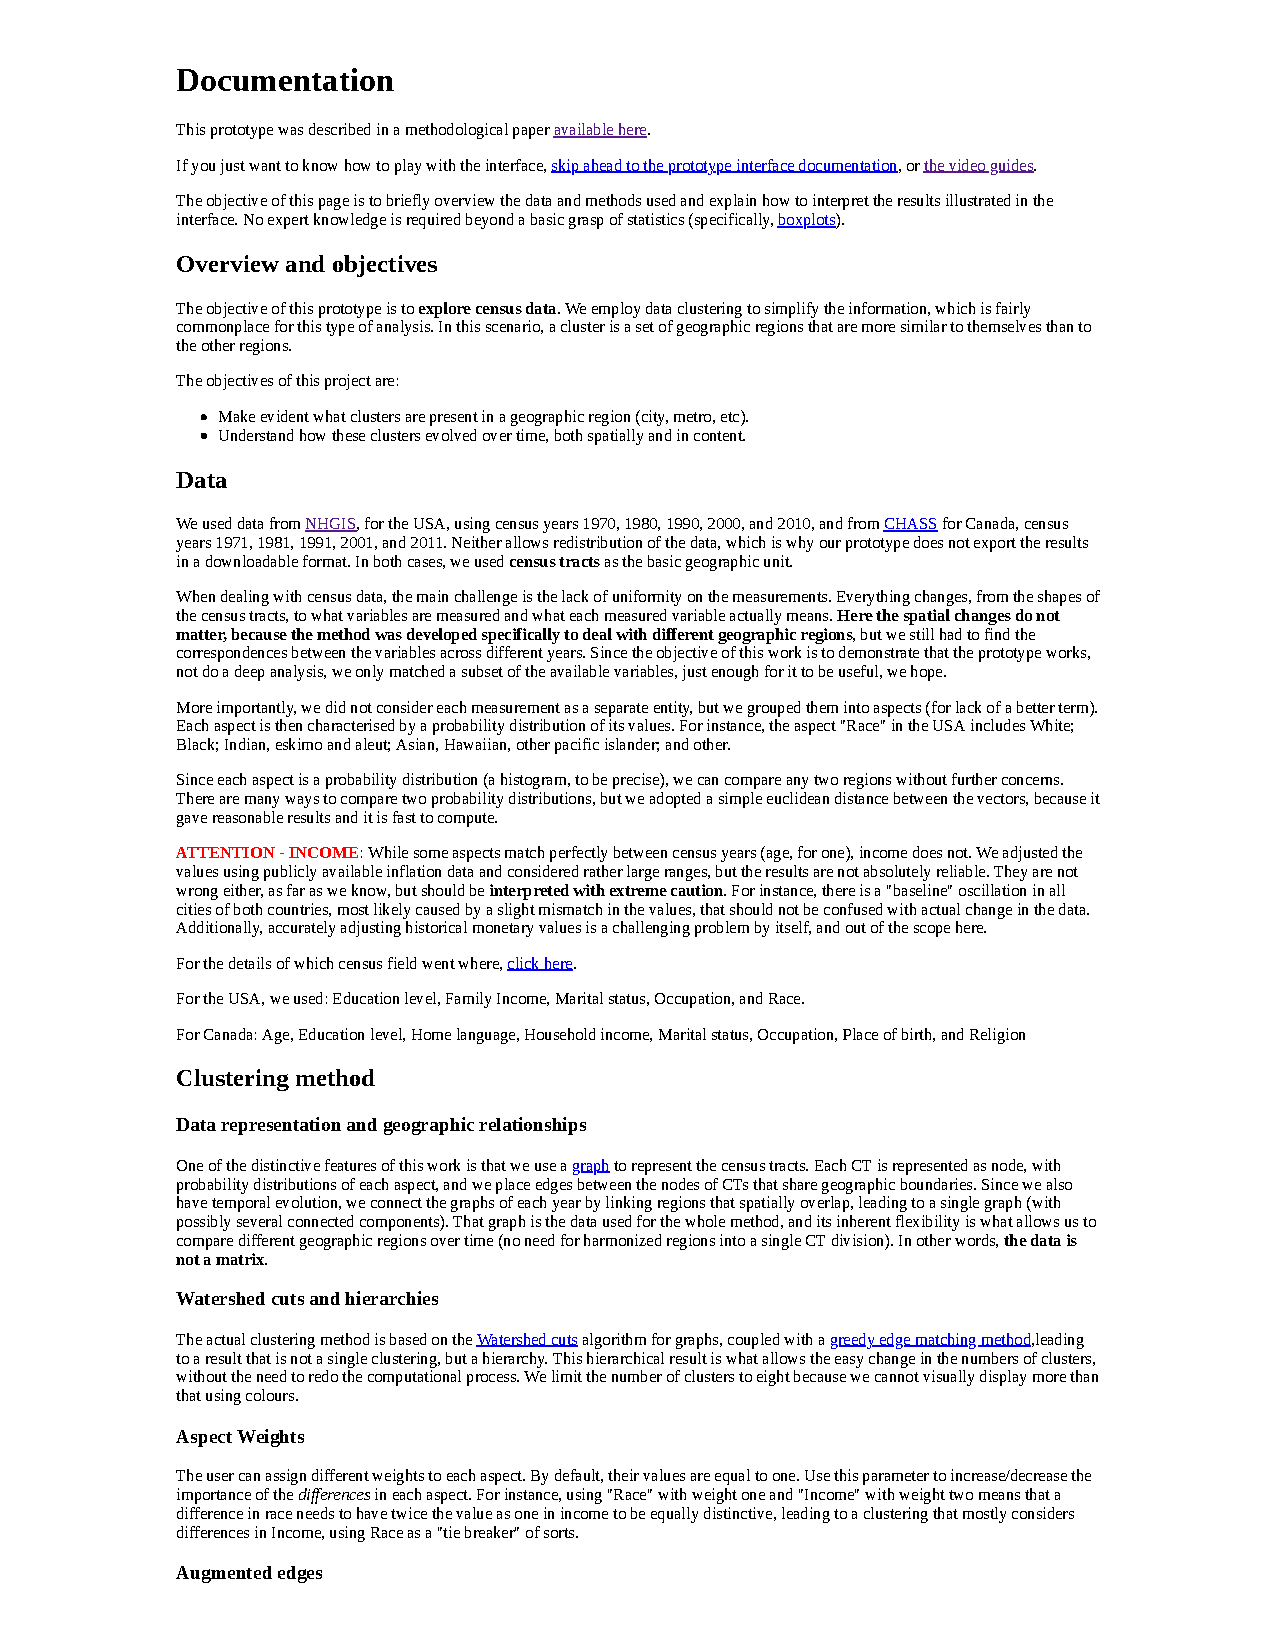
\includepdf[pages=-,pagecommand={},width=1.5\textwidth]{Documentation.pdf}

\subsection{A - Cary Wu}
%\href{https://soci.ubc.ca/persons/cary-wu/}{\url{https://soci.ubc.ca/persons/cary-wu/}}
\emph{Doctoral candidate in Sociology at the University of British Columbia, Canada.}

\question{Does this prototype make the exploration of census data easier?}
 

It definitely does! With the visualizations, we can tell many different stories
about neighborhoods/cities and their changes over time without doing the “dirty
work” of analyzing raw/big census data.
 

 

\question{By using it, did you find anything interesting? Either new insight or
something that demonstrates/disproves an established insight? }
 

This program demonstrates how specific combinations of local characteristics can
create distinctive or comparable scenes. As such, neighborhoods and cities can
be studied and compared in a way that the unit of sociological/urban analysis is
scenes.
 
 
\question{What questions would you be interested in pursuing further with this tool?}
 

We can perhaps develop measures based on cluster changes that could capture
whether a city or a neighborhood has become more diverse or homogeneous, and
also in terms of different aspects (e.g., race/ethnicity, SES, religion, and
immigration). It will also be interesting to explore whether different clusters
would shape other aspects of the neighborhoods and cities, such as trust, voting
pattern, and population movement.
 
 
\question{What would you add/remove/change on it?}
 

Instead of presenting everything on one overwhelming webpage (!), I would maybe
create multiple pages for different sections (e.g., configuration, choose
different cities), and embed them into one home page. Or maybe use popups for
results?
 
 
Overall, it is a very cool program, and I can see huge potential as a tool for
survey data visualization. For example, we can develop similar tools to
visualize the U.S. General Social Survey across different states from 1972-2016.


\subsection{B - Ethan Fosse}
% \href{https://scholar.harvard.edu/ethanfosse}{\url{https://scholar.harvard.edu/ethanfosse}}
\emph{Research Associate at Princeton University, USA}

Very cool visualization tool! To answer your questions:

\question{Does this prototype make the exploration of census data easier?}

Yes, absolutely. Census data can be difficult to download and clean, especially
for people who are not familiar with statistical software packages.

\question{By using it, did you find anything interesting? Either new insight or
something that demonstrates/disproves an established insight?}

I focused on Manhattan, since this is near where I currently live (Jersey City,
New Jersey). The visualization tool confirmed the gentrification of Manhattan,
with the exception of some areas (e.g., Chinatown and parts of the Lower East
Side). I'd like to know more about who lives in the Lower East Side. Is there a
conscious effort to resist gentrification in that part of the city, or is it
just a consequence of limited public transportation to the area, or is something
else going on?
 
\question{What questions would you be interested in pursuing further with this tool? }

I would like to see other data incorporated into the tool -- e.g., "cultural"
data involving consumption practices. Of course, it's no easy feat to obtain
these data, let alone merge into a geographic information system.

\question{What would you add/remove/change on it?}

Overall I enjoyed using the visualization tool and I found it easy to navigate.
I have two suggestions. First, I would work on speeding up the code that loads
the tool. Even after several minutes I could not load the Brooklyn data on
various browsers, for example. Second, as far as changes to the interface, my
only recommendation is to place the choice of various locations in a more
prominent place. Typically I think of the "Gear" icon as representing more
technical options, but the first change I made was altering the location.

\subsection{C - Fernando Calderón Figueroa}
\emph{Doctoral candidate in Sociology at the University of Toronto, Canada}


\textbf{Overall assessment}

As a first impression, I think the tool needs a brief summary of what it does
and how can people play with it. It took me a while between reading the
documentation and playing with it to make sense of what was going on underneath.
Maybe having a 5-minute tutorial would solve the problem, with someone (a voice
and captions) showing the user what’s going on in each section of the interface.
This has helped me in the past dealing with new software.

I really like the idea of the colours having the additional tag of the feature
that defines them more clearly on the left. However, once one starts playing
around with the platform using several variables at the same time, things become
tricky to interpret. For example, in Vancouver, things seem to change
dramatically from all green to all orange. This is highlighted by the graph of
trajectories in which the population involved in each cluster is nested in
colours. Once one gets into the data, the changes don't look so sharp after all
(maybe in education and income). This may not be a problem of the platform as it
is, but there may be a warning regarding that the “severity” of changes is not
necessarily the same across cities. 

Related to my previous point, in some cities the interpretation of the patterns
is clearer than in others. I think the platform works great in Montreal, for
instance. With a little knowledge about the city, the clustering makes a lot of
sense in how the composition has evolved. 

\textbf{Some specifics}

\begin{itemize}
    \item{For the boxplots, overlapping the gray ones in the back to show the
            difference with other clusters is a bit confusing, especially for
            those with no colour in them. Maybe a different colour or more
            transparency would help. }

    \item{I have trouble making sense of the top-right map. In the documentation
            it’s described as “the geographic positions of the trajectories,
            considering all years (the other maps show the clustering results
            for specific years).” While this is clear, it seems a little tricky
            to interpret. Is it the clustering adding all years together? Is it
            calculated as an average trajectory? How is that interpreted?
            Overall, I thought this to be a good summary map, but it has such an
            importance in the interface that I think obscures the fact that the
            maps below show, as a whole, how the trajectories move over time.}

    \item{If, as a user, I wanted to get a simple output for a presentation, it
            would be ideal to get the sequence of maps to show the changes over
            time. I could get a screenshot but providing it as a potential
            product would be very useful. A more sophisticated version would
            include a GIF image, but that may be harder to do and not so popular
            for other users beyond me.}
\end{itemize}


\subsection{D - Patrick Adler}
\emph{Research Associate at the Martin Prosperity Institute, Canada.}

\question{Does this prototype make the exploration of census data easier?}

The prototype allows me to visualize the relationship between key urban
variables over time and easily explore  what variables distinguish spaces from
each other. As someone who can’t make my own maps, I usually have to wait until
the end of a project before I start to commission visuals. I only have the
luxury of visualizing data that I fully understand (or think I fully understand
at least).  This tool allows me to use visualization as a tool in my own
research process.  

 

\question{By using it, did you find anything interesting? Either new insight or
 something that demonstrates/disproves an established insight? What questions
 would you be interested in pursuing further with this tool? }

 
The spatial analysis  supports speculative reasoning from [1] about the return
to central cities and central business districts of moneyed, educated, knowledge
workers. They hypothesized that this transition happened over the past 20 years
and  that it is more complete in a set of metros with high levels of
‘post-industrialism’. The tools helps to verify this analysis and show that
occupational clustering is robust in many cities, even when orthogonal measures
are added.  This tool can be used to formally extend the analysis to the full
range of metros.


\noindent [1]: \href{https://www.tandfonline.com/doi/abs/10.1080/07352166.2017.1360743}{\url{https://www.tandfonline.com/doi/abs/10.1080/07352166.2017.1360743}}


\question{What would you add/remove/change on it?}
\begin{enumerate}
  \item{More summary statistics about the clusters would be very useful (density,
  population, distance from transit etc)}
  \item{A tool that would allow us to  point to a cluster and find similar clusters in
  other neighborhoods would be most useful.}
  \item{It would be great to have a quick way to snap pictures, as well as a
  tool to export data in to CSV}
  \item{We would appreciate the ability to restrict the analysis to an interval
  within. For the analysis above 2000-2010 might be useful}
  \item{Processing speed is an issue that I'm sure will be resolved in time}
\end{enumerate}



\subsection{E - James Murdoch}
\emph{Policy Analyst at 2M Research, USA}

Wow!! This is quite an undertaking and I definitely see the potential of this
tool for understanding neighborhood dynamics overtime. Here are some uses I see

It offers a quick way to identify particular neighborhoods (i.e. Census tracts)
that one may be interested in studying more in depth around a particular issue.
A good example is gentrification. I was able to use the tool to identify several
neighborhoods in Dallas that I know have gentrified over the years by looking at
how race/education/income changed since 1970. You can also easily see when the
neighborhood “tipped” as the cluster color will change. That is quite a feat as
without this tool just getting all the necessary data is a lot of work. Plus
being able to see a neighborhood change from black dominated to white dominated,
for example, is really powerful. Its really a nice tool for efficiently
understanding the context of an area. In a program evaluation of some kind of
place-based intervention this tool would be a great way to produce data on the
context in which the intervention is occurring. I could also see it facilitating
descriptive analysis that provides some evidence of how an intervention may
impact a particular place as the tool allows for the analysis of trends. I think
it could be an excellent planning tool for local governments. As more data is
added, the tool will be able to quickly show clusters of particular types of
economic activity, cultural activity, types of residents and consumers, and many
other things that planners may be interested in. It could also serve as a
communication tool for more participatory planning. For example, you could take
an asset-based approach where you highlight the resources in the neighborhood
with the tool and ask residents to react, offer insight, and make suggestions
how to capitalize on what already exists in a neighborhood or city.
 

Some questions:
\begin{itemize}
\item{Do you think users will ever be able to import their own data? For
example, what if someone had violent crime data from the local police department
that they want to overlay with the other data in the tool. Will that be possible
at some point?}

\item{I know you can’t export raw data, but what about the ability to save a
customized map or some type of data graphic? That would be super useful for
people that need to write reports or do a presentation.}

\item{Any ambitions to include social media info or other “big data” sources
similar to that in here?}
\end{itemize} 

A couple criticisms:

\begin{itemize}
  
  \item{Obviously the tool is still buggy. I had to restart several times. Also
  it would be nice if the big map in the top right also moved the smaller maps
  that correspond to different time points just below it. I notice that moving
  one of the smaller maps moves all the other smaller maps, but moving the big
  map doesn’t do anything. Also I didn’t see a way to enlarge the map. I’d like
  to be able to have a full screen view of the map that I can toggle when
  needed.}
  
  \item{It is a little intimidating at first. I might recommend starting with a
  simpler default (only one variable, less than 5 clusters, etc.) and allow
  people to work up in complexity if they want to. I found it a bit hard to get
  in to it as I had to really think about what I was looking at first.}
\end{itemize}

I really must commend you on your work. This is an amazing tool that you have
put together. Great job and thanks for sharing this with me!! Please keep me
updated as you develop it further. I could definitely see a use for it in the
work I do both in my personal research and at my work at 2M.



\clearpage
\section{Data samples}
\subsection{Canada}
Data for one CT over time in Toronto.
\begin{center}
  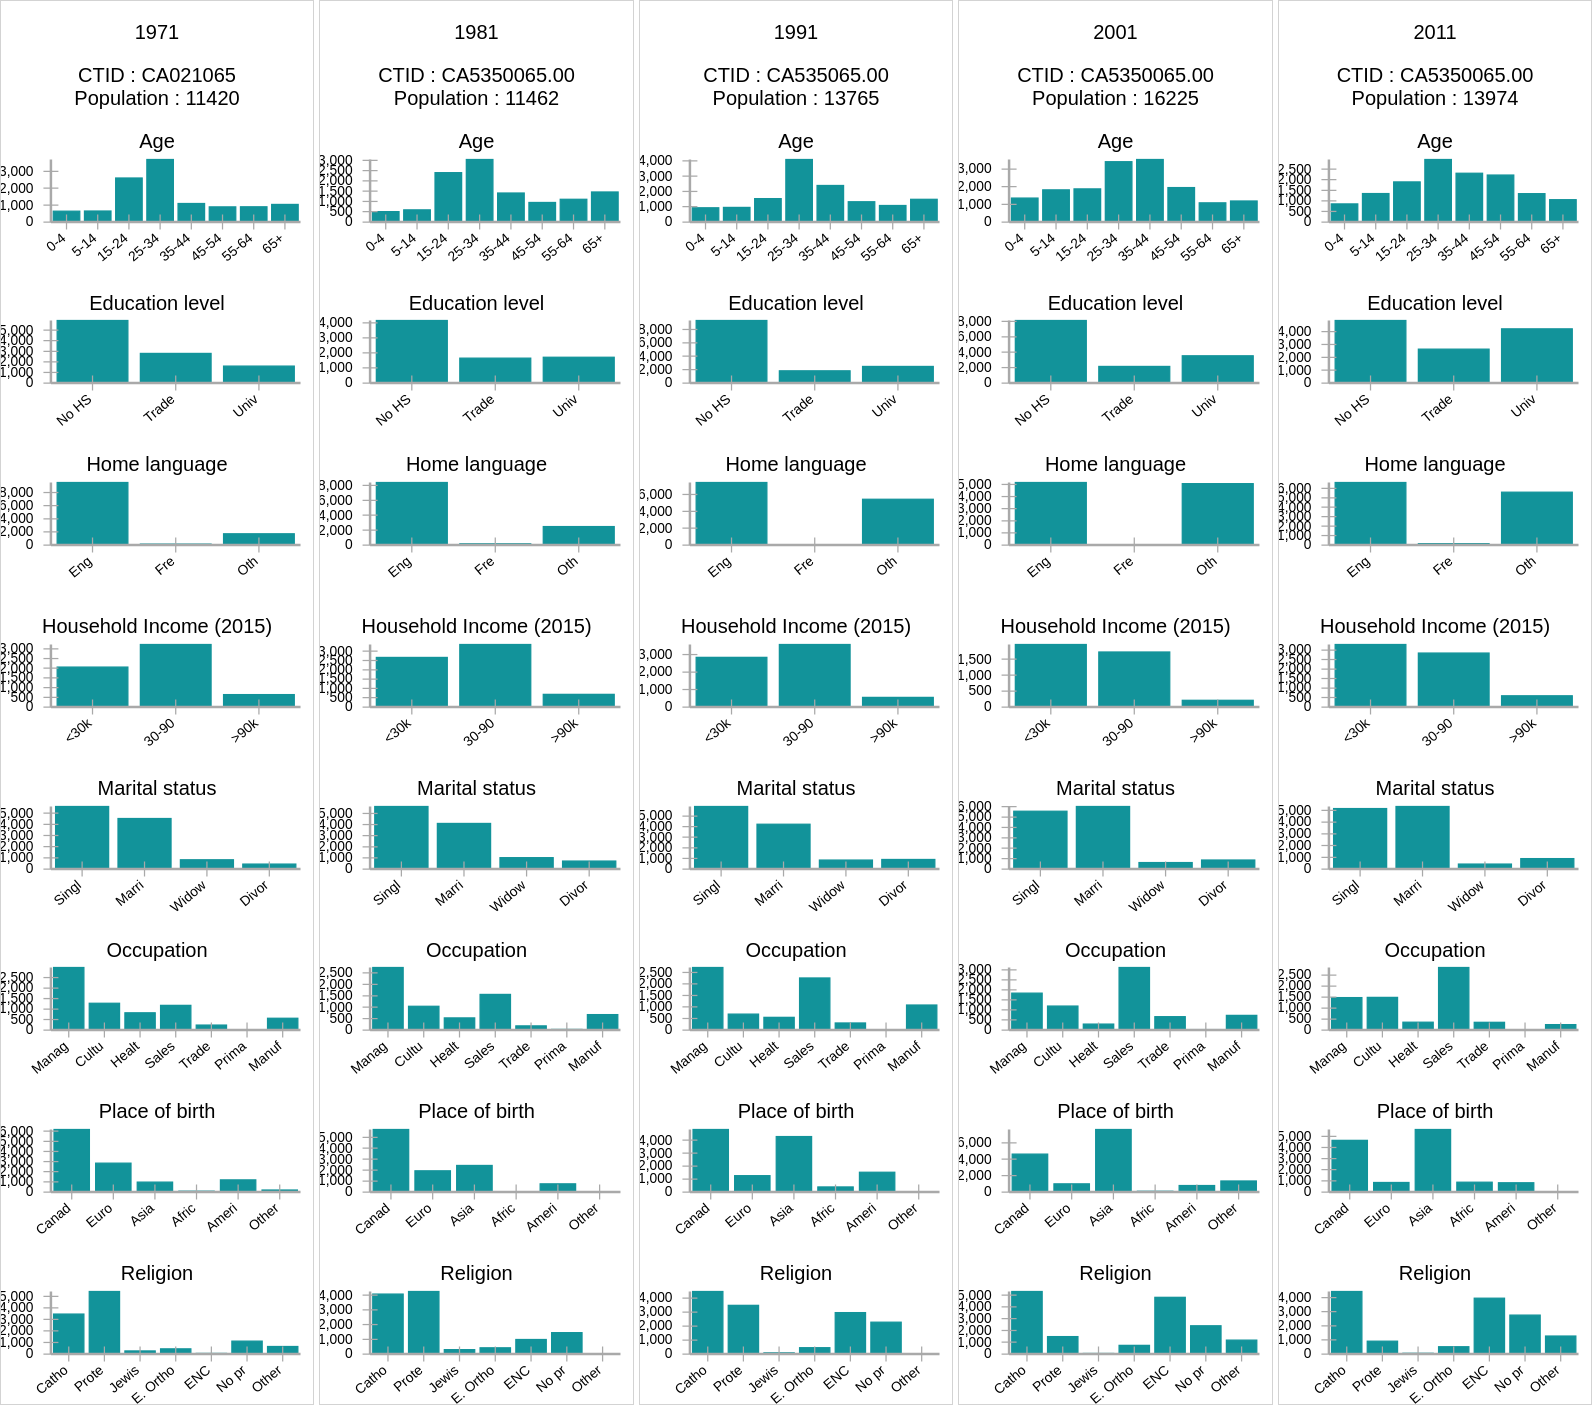
\includegraphics[width=\linewidth]{SampleCA.png}
  \begin{tabular}{lccccc}
	\hline
	Home language&1971&1981&1991&2001&2011\\
	\hline
	 English & 9530&8390&7420&5160&6615 \\
	 French & 135&155&40&25&135 \\
	 Other & 1710&2475&5430&5065&5590 \\
	\hline
	Population&1971&1981&1991&2001&2011\\
	\hline
	 Total & 11420&11462&13765&16225&13974 \\
	\hline
	Age&1971&1981&1991&2001&2011\\
	\hline
	 0-4 & 640&505&930&1355&855 \\
	 5-14 & 650&590&955&1820&1345 \\
	 15-24 & 2605&2400&1530&1875&1895 \\
	 25-34 & 3700&3040&4090&3415&2955 \\
	 35-44 & 1095&1410&2390&3540&2305 \\
	 45-54 & 895&950&1325&1950&2220 \\
	 55-64 & 900&1105&1080&1085&1340 \\
	 65 and over & 1040&1460&1485&1190&1055 \\
	\hline
	Education level&1971&1981&1991&2001&2011\\
	\hline
	 HS or below & 5915&4150&9340&8110&4865 \\
	 Trades or college & 2800&1650&1820&2150&2635 \\
	 University & 1600&1710&2475&3530&4215 \\
	\hline
	Occupation&1971&1981&1991&2001&2011\\
	\hline
	 Managerial and business support & 2980&2740&2715&1840&1475 \\
	 Culture & 1275&1040&690&1195&1485 \\
	 Health & 820&530&550&295&355 \\
	 Sales and service & 1175&1560&2260&3120&2845 \\
	 Trades and construction & 235&180&305&665&350 \\
	 Primary & 10&25&10&20&0 \\
	 Manufacturing & 560&675&1085&730&245 \\
	\hline
	Religion&1971&1981&1991&2001&2011\\
	\hline
	 Catholic & 3460&4070&4470&5315&4435 \\
	 Protestant & 5415&4245&3480&1480&910 \\
	 Jewish & 265&295&80&45&50 \\
	 Eastern Orthodox & 445&420&450&735&515 \\
	 Eastern non-christian & 50&985&2960&4820&3960 \\
	 No preference & 1115&1450&2275&2400&2760 \\
	 Other & 650&25&25&1180&1275 \\
	\hline
	Household Income (2015)&1971&1981&1991&2001&2011\\
	\hline
	 30k and less & 2060&2665&2840&1960&3290 \\
	 30-90k & 3225&3360&3575&1725&2840 \\
	 90k and more & 640&680&550&210&590 \\
	\hline
	Marital status&1971&1981&1991&2001&2011\\
	\hline
	 Single & 5595&5625&5905&5560&5145 \\
	 Married (incl. separated) & 4520&4100&4230&6015&5320 \\
	 Widowed & 825&1020&845&620&420 \\
	 Divorced & 440&715&900&865&885 \\
	\hline
	Place of birth&1971&1981&1991&2001&2011\\
	\hline
	 Canada & 6165&5710&4825&4625&4640 \\
	 Europe & 2845&1935&1260&995&855 \\
	 Asia & 975&2425&4280&7630&5615 \\
	 Africa & 80&0&390&90&880 \\
	 Americas & 1195&745&1525&790&830 \\
	 Other & 195&0&15&1345&0 \\
\end{tabular}

  \end{center}   

\clearpage

\subsection{USA}
Data for one CT over time in Brooklyn.
\begin{center}
  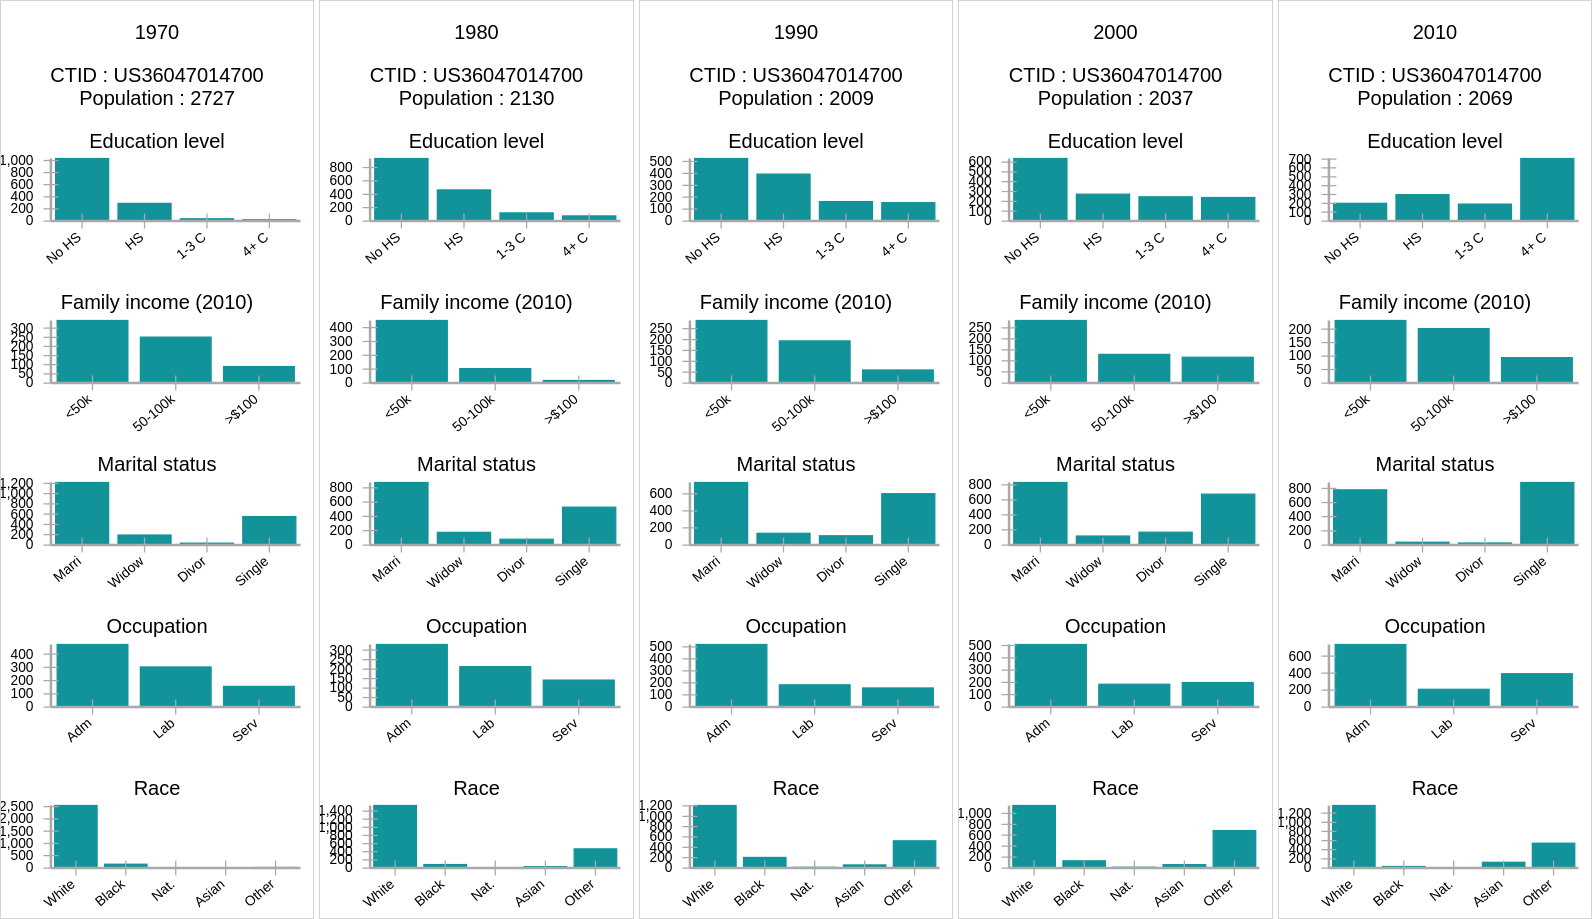
\includegraphics[width=\linewidth]{SampleUS.png}
  \begin{tabular}{lccccc}
	\hline
	Population&1970&1980&1990&2000&2010\\
	\hline
	 Total & 2727&2130&2009&2037&2069 \\
	\hline
	Race&1970&1980&1990&2000&2010\\
	\hline
	 White & 2550&1537&1208&1145&1368 \\
	 Black & 154&85&204&131&33 \\
	 Indian, eskimo and aleut & 0&4&13&14&0 \\
	 Asian, Hawaiian, other pacific islander & 2&34&59&61&125 \\
	 Other & 21&470&525&686&543 \\
	\hline
	Marital status&1970&1980&1990&2000&2010\\
	\hline
	 Married (inc. Sep.) & 1217&874&732&831&780 \\
	 Widowed & 194&177&137&119&39 \\
	 Divorced & 36&80&108&170&28 \\
	 Never married & 554&529&601&676&884 \\
	\hline
	Education level&1970&1980&1990&2000&2010\\
	\hline
	 Not completed High School & 1033&936&525&636&200 \\
	 High School & 291&465&394&273&298 \\
	 College 1-3 years & 36&121&163&246&191 \\
	 College 4+ years & 20&76&154&239&707 \\
	\hline
	Family income (2010)&1970&1980&1990&2000&2010\\
	\hline
	 50k and less & 342&452&288&284&232 \\
	 50k-100k & 251&104&194&130&202 \\
	 100k and more & 90&18&60&117&94 \\
	\hline
	Occupation&1970&1980&1990&2000&2010\\
	\hline
	 Administrative & 473&330&519&508&738 \\
	 Laborers & 303&213&184&185&209 \\
	 Service & 156&142&158&199&393 \\
\end{tabular}

\end{center} 

\end{document}

\clearpage
\section{Variable matching} 

The following listing contains the fields that were added to form the aspects.
If the name of a field starts with "(-)", it means that this field was
subtracted.


\subsection{Canada}
\subsubsection{Home language}
\paragraph{English}
\begin{itemize}
   \item{\textbf{1971}:  Home language: English;}
   \item{\textbf{1981}:  Home language - - English home language; Home language - - English home language; Home language - - English home language;}
   \item{\textbf{1991}:  English, home language;}
   \item{\textbf{2001}:  English;}
   \item{\textbf{2011}:  Detailed language spoken most often at home - Both sexes / Total population excluding institutional residents, Both sexes / Single responses, Both sexes / English, Both sexes;}
\end{itemize}

\paragraph{French}
\begin{itemize}
   \item{\textbf{1971}:  Home language: French;}
   \item{\textbf{1981}:  Home language - - French home language; Home language - - French home language; Home language - - French home language;}
   \item{\textbf{1991}:  French, home language;}
   \item{\textbf{2001}:  French;}
   \item{\textbf{2011}:  Detailed language spoken most often at home - Both sexes / Total population excluding institutional residents, Both sexes / Single responses, Both sexes / French, Both sexes;}
\end{itemize}

\paragraph{Other}
\begin{itemize}
   \item{\textbf{1971}:  Home language: other;}
   \item{\textbf{1981}:  Home language - - home language same as mother tongue;}
   \item{\textbf{1991}:  Non-official languages, home language;}
   \item{\textbf{2001}:  Non-official languages;}
   \item{\textbf{2011}:  Detailed language spoken most often at home - Both sexes / Total population excluding institutional residents, Both sexes / Single responses, Both sexes / Non-official languages, Both sexes;}
\end{itemize}

\subsubsection{Population}
\paragraph{Total}
\begin{itemize}
   \item{\textbf{1971}:  Total population;}
   \item{\textbf{1981}:  Population, 1981;}
   \item{\textbf{1991}:  Total population;}
   \item{\textbf{2001}:  Population, 2001 - 100\% Data;}
   \item{\textbf{2011}:  Population and dwelling counts / Population, 2011;}
\end{itemize}

\subsubsection{Age}
\paragraph{0-4}
\begin{itemize}
   \item{\textbf{1971}:  Population: males: 0-4 years of age; Population: females: 0-4 years of age;}
   \item{\textbf{1981}:  Males, 0 - 4 years; Females, 0 - 4 years;}
   \item{\textbf{1991}:  Males, 0 - 4 years; Females, 0 - 4 years;}
   \item{\textbf{2001}:  0-4; 0-4;}
   \item{\textbf{2011}:  Age \& Sex - Both sexes / Total population by age groups, Both sexes / 0 to 4 years, Both sexes;}
\end{itemize}

\paragraph{5-14}
\begin{itemize}
   \item{\textbf{1971}:  Population: males: 10-14 years of age; Population: females: 10-14 years of age; Population: males: 5-9 years of age; Population: females: 5-9 years of age;}
   \item{\textbf{1981}:  Males, 10 - 14 years; Females, 10 - 14 years; Males, 5 - 9 years; Females, 5 - 9 years;}
   \item{\textbf{1991}:  Males, 10 - 14 years; Females, 10 - 14 years; Males, 5 - 9 years; Females, 5 - 9 years;}
   \item{\textbf{2001}:  10-14; 10-14; 5-9; 5-9;}
   \item{\textbf{2011}:  Age \& Sex - Both sexes / Total population by age groups, Both sexes / 10 to 14 years, Both sexes; Age \& Sex - Both sexes / Total population by age groups, Both sexes / 5 to 9 years, Both sexes;}
\end{itemize}

\paragraph{15-24}
\begin{itemize}
   \item{\textbf{1971}:  Population: males: 15 years of age; Population: males: 16 years of age; Population: males: 17 years of age; Population: males: 18-19 years of age; Population: females: 15 years of age; Population: females: 16 years of age; Population: females: 17 years of age; Population: females: 18-19 years of age; Population: males: 20-24 years of age; Population: females: 20-24 years of age;}
   \item{\textbf{1981}:  Males, 15 - 19 years; Females, 15 - 19 years; Males, 20 - 24 years; Females, 20 - 24 years;}
   \item{\textbf{1991}:  Males, 15 - 19 years; Females, 15 - 19 years; Males, 20 - 24 years; Females, 20 - 24 years;}
   \item{\textbf{2001}:  15-19; 15-19; 20-24; 20-24;}
   \item{\textbf{2011}:  Age \& Sex - Both sexes / Total population by age groups, Both sexes / 15 to 19 years, Both sexes; Age \& Sex - Both sexes / Total population by age groups, Both sexes / 20 to 24 years, Both sexes;}
\end{itemize}

\paragraph{25-34}
\begin{itemize}
   \item{\textbf{1971}:  Population: males: 25-29 years of age; Population: males: 30-34 years of age; Population: females: 25-29 years of age; Population: females: 30-34 years of age;}
   \item{\textbf{1981}:  Males, 25 - 34 years; Females, 25 - 34 years;}
   \item{\textbf{1991}:  Males, 25 - 29 years; Males, 30 - 34 years; Females, 25 - 29 years; Females, 30 - 34 years;}
   \item{\textbf{2001}:  25-29; 30-34; 25-29; 30-34;}
   \item{\textbf{2011}:  Age \& Sex - Both sexes / Total population by age groups, Both sexes / 25 to 29 years, Both sexes; Age \& Sex - Both sexes / Total population by age groups, Both sexes / 30 to 34 years, Both sexes;}
\end{itemize}

\paragraph{35-44}
\begin{itemize}
   \item{\textbf{1971}:  Population: males: 35-39 years of age; Population: males: 40-44 years of age; Population: females: 35-39 years of age; Population: females: 40-44 years of age;}
   \item{\textbf{1981}:  Males, 35 - 44 years; Females, 35 - 44 years;}
   \item{\textbf{1991}:  Males, 35 - 39 years; Males, 40 - 44 years; Females, 35 - 39 years; Females, 40 - 44 years;}
   \item{\textbf{2001}:  35-39; 40-44; 35-39; 40-44;}
   \item{\textbf{2011}:  Age \& Sex - Both sexes / Total population by age groups, Both sexes / 35 to 39 years, Both sexes; Age \& Sex - Both sexes / Total population by age groups, Both sexes / 40 to 44 years, Both sexes;}
\end{itemize}

\paragraph{45-54}
\begin{itemize}
   \item{\textbf{1971}:  Population: males: 45-49 years of age; Population: males: 50-54 years of age; Population: females: 45-49 years of age; Population: females: 50-54 years of age;}
   \item{\textbf{1981}:  Males, 45 - 54 years; Females, 45 - 54 years;}
   \item{\textbf{1991}:  Males, 45 - 49 years; Males, 50 - 54 years; Females, 45 - 49 years; Females, 50 - 54 years;}
   \item{\textbf{2001}:  45-49; 50-54; 45-49; 50-54;}
   \item{\textbf{2011}:  Age \& Sex - Both sexes / Total population by age groups, Both sexes / 45 to 49 years, Both sexes; Age \& Sex - Both sexes / Total population by age groups, Both sexes / 50 to 54 years, Both sexes;}
\end{itemize}

\paragraph{55-64}
\begin{itemize}
   \item{\textbf{1971}:  Population: males: 55-59 years of age; Population: males: 60-64 years of age; Population: females: 55-59 years of age; Population: females: 60-64 years of age;}
   \item{\textbf{1981}:  Males, 55 - 64 years; Females, 55 - 64 years;}
   \item{\textbf{1991}:  Males, 55 - 59 years; Males, 60 - 64 years; Females, 55 - 59 years; Females, 60 - 64 years;}
   \item{\textbf{2001}:  55-59; 60-64; 55-59; 60-64;}
   \item{\textbf{2011}:  Age \& Sex - Both sexes / Total population by age groups, Both sexes / 55 to 59 years, Both sexes; Age \& Sex - Both sexes / Total population by age groups, Both sexes / 60 to 64 years, Both sexes;}
\end{itemize}

\paragraph{65 and over}
\begin{itemize}
   \item{\textbf{1971}:  Population: males: 65-69 years of age; Population: males: 70 years of age and over; Population: females: 65-69 years of age; Population: females: 70 years of age and over;}
   \item{\textbf{1981}:  Males, 65 - 69 years; Males, 70 years and over; Females, 65 - 69 years; Females, 70 years and over;}
   \item{\textbf{1991}:  Males, 65 - 74 years; Males, 75 - 84 years; Males, 85 years and over; Females, 65 - 74 years; Females, 75 - 84 years; Females, 85 years and over;}
   \item{\textbf{2001}:  65-69; 70-74; 75-79; 80-84; 85+; 65-69; 70-74; 75-79; 80-84; 85+;}
   \item{\textbf{2011}:  Age \& Sex - Both sexes / Total population by age groups, Both sexes / 65 to 69 years, Both sexes; Age \& Sex - Both sexes / Total population by age groups, Both sexes / 70 to 74 years, Both sexes; Age \& Sex - Both sexes / Total population by age groups, Both sexes / 75 to 79 years, Both sexes; Age \& Sex - Both sexes / Total population by age groups, Both sexes / 80 to 84 years, Both sexes; Age \& Sex - Both sexes / Total population by age groups, Both sexes / 85 years and over, Both sexes;}
\end{itemize}

\subsubsection{Education level}
\paragraph{HS or below}
\begin{itemize}
   \item{\textbf{1971}:  Pop 5 yrs+: highest level schooling: grade 11-13: no other t; Pop 5 yrs+: highest level schooling: some university: no oth; Pop 5 yrs+: highest level schooling: less than grade 9; Pop 5 yrs+: highest level schooling: grade 9-10: no other tr; (-)  Population: males: 10-14 years of age; (-)  Population: females: 10-14 years of age; (-)  Population: males: 5-9 years of age; (-)  Population: females: 5-9 years of age;}
   \item{\textbf{1981}:  Highest level of schooling: grades 9-13 with secondary certificate; Highest level of schooling: other non-university education only(11)- without certificate; Highest level of schooling: grades 9-13 without secondary certificate;}
   \item{\textbf{1991}:  Population 15+ years - Grades 9-13 - With secondary certificate; Population 15+ years - Other non-university - Without certificate; Population 15+ years - University - Without degree; Population 15+ years - University - Without certificate; Population 15+ years - Highest level of schooling, less than grade 9; Population 15+ years - Grades 9-13 - Without secondary certificate;}
   \item{\textbf{2001}:  With high school graduation certificate; Without certificate or diploma; Without degree; Without certificate or diploma; Less than grade 9; Without high school graduation certificate;}
   \item{\textbf{2011}:  Education - Both sexes / Total population aged 15 years and over by highest certificate, diploma or degree, Both sexes / High school diploma or equivalent, Both sexes; 
                         Education - Both sexes / Total population aged 15 years and over by highest certificate, diploma or degree, Both sexes / No certificate, diploma or degree, Both sexes;}
\end{itemize}

\paragraph{Trades or college}
\begin{itemize}
   \item{\textbf{1971}:  Pop 5 yrs+: highest level schooling: grade 9-10: \& other tra; Pop 5 yrs+: highest level schooling: grade 11-13: \& other tr; Pop 5 yrs+: highest level schooling: some university: \& othe;}
   \item{\textbf{1981}:  Highest level of schooling: trades certificate or diploma; Highest level of schooling: other non-university education only- with certificate(12);}
   \item{\textbf{1991}:  Population 15+ years - Trades certificate or diploma; Population 15+ years - Other non-university - With certificate;}
   \item{\textbf{2001}:  Trades certificate or diploma; With certificate or diploma;}
   \item{\textbf{2011}:  Education - Both sexes / Total population aged 15 years and over by highest certificate, diploma or degree, Both sexes / Postsecondary certificate, diploma or degree, Both sexes / Apprenticeship or trades certificate or diploma, Both sexes; Education - Both sexes / Total population aged 15 years and over by highest certificate, diploma or degree, Both sexes / Postsecondary certificate, diploma or degree, Both sexes / College, CEGEP or other non-university certificate or diploma, Both sexes;}
\end{itemize}

\paragraph{University}
\begin{itemize}
   \item{\textbf{1971}:  Pop 5 yrs+: highest level schooling: univ degree: no other t; Pop 5 yrs+: highest level schooling: univ degree: \& other tr;}
   \item{\textbf{1981}:  Highest level of schooling: university(13)- with degree;}
   \item{\textbf{1991}:  Population 15+ years - University - With certificate; Population 15+ years - University - With degree;}
   \item{\textbf{2001}:  With certificate or diploma; With bachelors degree or higher;}
   \item{\textbf{2011}:  Education - Both sexes / Total population aged 15 years and over by highest certificate, diploma or degree, Both sexes / Postsecondary certificate, diploma or degree, Both sexes / University certificate or diploma below bachelor level, Both sexes; 
                         Education - Both sexes / Total population aged 15 years and over by highest certificate, diploma or degree, Both sexes / Postsecondary certificate, diploma or degree, Both sexes / University certificate, diploma or degree at bachelor level or above, Both sexes;}
\end{itemize}

\subsubsection{Occupation}
\paragraph{Managerial and business support}
\begin{itemize}
   \item{\textbf{1971}:  Managerial, admin \& related occupations: males; Managerial, administrative \& related occupations: females; Clerical \& related: males; Clerical \& related occupations: females;}
   \item{\textbf{1981}:  Occupation major groups(18): males - managerial, administrative and related occupations; Occupation major groups(18): females - managerial, administrative and related occupations; Occupation major groups(18): males - clerical and related occupations; Occupation major groups(18): females - clerical and related occupations;}
   \item{\textbf{1991}:  Males, Managerial, administrative and related occupations; Females, Managerial, administrative and related occupations; Males, Clerical and related occupations; Females, Clerical and related occupations;}
   \item{\textbf{2001}:  A Management occupations; B Business, finance and administration occupations;}
   \item{\textbf{2011}:  Occupation - Both sexes / Total labour force population aged 15 years and over by occupation - National Occupational Classification (NOC) 2011, Both sexes / All occupations, Both sexes / 0 Management occupations, Both sexes; Occupation - Both sexes / Total labour force population aged 15 years and over by occupation - National Occupational Classification (NOC) 2011, Both sexes / All occupations, Both sexes / 1 Business, finance and administration occupations, Both sexes;}
\end{itemize}

\paragraph{Culture}
\begin{itemize}
   \item{\textbf{1971}:  Technological, social, religious, artistic occupations: male; Technological, social, religious, artistic occupations: fema; Teaching \& related occupations: males; Teaching \& related occupations: females;}
   \item{\textbf{1981}:  Occupation major groups(18): males - teaching and related occupations; Occupation major groups(18): males - technological, social, religious, artistic and related occupations (21); Occupation major groups(18): females - teaching and related occupations; Occupation major groups(18): females - technological, social, religious, artistic \& related occupations(21);}
   \item{\textbf{1991}:  Males, Occupations in nat. sciences, engineering and math.; ales, Occupations in social sciences and related fields; Males, Occupations in religion; Males, Teaching and related occupations; Males, Artistic, literary, recreational and related occs.; Females, Occupations in nat. sciences, engineering and math.; Females, Occupations in social sciences and related fields; Females, Occupations in religion; Females, Teaching and related occupations; Females, Artistic, literary, recreational and related occs.;}
   \item{\textbf{2001}:  C Natural and applied sciences and related occupations; E Occupations in social science, education, government service and religion; F Occupations in art, culture, recreation and sport;}
   \item{\textbf{2011}:  Occupation - Both sexes / Total labour force population aged 15 years and over by occupation - National Occupational Classification (NOC) 2011, Both sexes / All occupations, Both sexes / 2 Natural and applied sciences and related occupations, Both sexes; Occupation - Both sexes / Total labour force population aged 15 years and over by occupation - National Occupational Classification (NOC) 2011, Both sexes / All occupations, Both sexes / 4 Occupations in education, law and social, community and government services, Both sexes; Occupation - Both sexes / Total labour force population aged 15 years and over by occupation - National Occupational Classification (NOC) 2011, Both sexes / All occupations, Both sexes / 5 Occupations in art, culture, recreation and sport, Both sexes;}
\end{itemize}

\paragraph{Health}
\begin{itemize}
   \item{\textbf{1971}:  Medicine \& health occupations: males; Medicine \& health occupations: females;}
   \item{\textbf{1981}:  Occupation major groups(18): males - occupations in medicine and health; Occupation major groups(18): females - occupations in medicine and health;}
   \item{\textbf{1991}:  Males, Occupations in medicine and health; Females, Occupations in medicine and health;}
   \item{\textbf{2001}:  D Health occupations;}
   \item{\textbf{2011}:  Occupation - Both sexes / Total labour force population aged 15 years and over by occupation - National Occupational Classification (NOC) 2011, Both sexes / All occupations, Both sexes / 3 Health occupations, Both sexes;}
\end{itemize}

\paragraph{Sales and service}
\begin{itemize}
   \item{\textbf{1971}:  Sales occupations: males; Service occupations: males; Sales occupations: females; Service occupations: females;}
   \item{\textbf{1981}:  Occupation major groups(18): males - sales occupations; Occupation major groups(18): males - service occupations; Occupation major groups(18): females - sales occupations; Occupation major groups(18): females - service occupations;}
   \item{\textbf{1991}:  Males, Sales occupations; Males, Service occupations; Females, Sales occupations; Females, Service occupations;}
   \item{\textbf{2001}:  G Sales and service occupations;}
   \item{\textbf{2011}:  Occupation - Both sexes / Total labour force population aged 15 years and over by occupation - National Occupational Classification (NOC) 2011, Both sexes / All occupations, Both sexes / 6 Sales and service occupations, Both sexes;}
\end{itemize}

\paragraph{Trades and construction}
\begin{itemize}
   \item{\textbf{1971}:  Construction trade occupations: males; Transport equipment operating occupations: males; Construction trade occupations: females; Transport equipment operating occupations: females;}
   \item{\textbf{1981}:  Occupation major groups(18): males - construction trades occupations; Occupation major groups(18): males - transport equipment operating occupations;}
   \item{\textbf{1991}:  Males, Construction trades occupations; Males, Transport equipment operating occupations; Females, Construction trades occupations; Females, Transport equipment operating occupations;}
   \item{\textbf{2001}:  H Trades, transport and equipment operators and related occupations;}
   \item{\textbf{2011}:  Occupation - Both sexes / Total labour force population aged 15 years and over by occupation - National Occupational Classification (NOC) 2011, Both sexes / All occupations, Both sexes / 7 Trades, transport and equipment operators and related occupations, Both sexes;}
\end{itemize}

\paragraph{Primary}
\begin{itemize}
   \item{\textbf{1971}:  Fishing \& hunting, forestry, mining, etc. occupations: males; Fishing \& hunting, forestry, mining, etc occupations: female;}
   \item{\textbf{1981}:  Occupation major groups(18): males - primary occupations(22); Occupation major groups(18): females - primary occupations(22);}
   \item{\textbf{1991}:  Males, Farming, horticultural and animal husbandry occs.; Males, Fishing, trapping and related occupations; Males, Forestry and logging occupations; Males, Mining \& quarrying incl. oil \& gas field occs.; Females, Farming, horticultural and animal husbandry occs.; Females, Fishing, trapping and related occupations; Females, Forestry and logging occupations; Females, Mining \& quarrying incl. oil \& gas field occs.;}
   \item{\textbf{2001}:  I Occupations unique to primary industry;}
   \item{\textbf{2011}:  Occupation - Both sexes / Total labour force population aged 15 years and over by occupation - National Occupational Classification (NOC) 2011, Both sexes / All occupations, Both sexes / 8 Natural resources, agriculture and related production occupations, Both sexes;}
\end{itemize}

\paragraph{Manufacturing}
\begin{itemize}
   \item{\textbf{1971}:  Processing occupations: males; Machining and related occupations: males; Processing occupations: females; Machining and related occupations: females;}
   \item{\textbf{1981}:  Occupation major groups(18): males - processing occupations; Occupation major groups(18): males - machining, product fabricating, assembling, and repairing occupations(23); Occupation major groups(18): females - processing occupations; Occupation major groups(18): females - machining, product fabricating, assemblng \& repairing occs(23);}
   \item{\textbf{1991}:  Males, Processing occupations; Males, Machining and related occupations; Males, Product fabricating, assembling \& repairing occs.; Males, Material handling and related occupations, n.e.c.; Males, Other crafts and equipment operating occupations; Females, Product fabricating, assembling \& repairing occs.; Females, Material handling and related occupations, n.e.c.; Females, Other crafts and equipment operating occupations;}
   \item{\textbf{2001}:  J Occupations unique to processing, manufacturing and utilities;}
   \item{\textbf{2011}:  Occupation - Both sexes / Total labour force population aged 15 years and over by occupation - National Occupational Classification (NOC) 2011, Both sexes / All occupations, Both sexes / 9 Occupations in manufacturing and utilities, Both sexes;}
\end{itemize}

\subsubsection{Religion}
\paragraph{Catholic}
\begin{itemize}
   \item{\textbf{1971}:  Religion: Roman Catholic; Religion: Ukrainian Catholic;}
   \item{\textbf{1981}:  Religion - Catholic;}
   \item{\textbf{1991}:  Religion, Catholic, total;}
   \item{\textbf{2001}:  Roman Catholic; Ukrainian Catholic;}
   \item{\textbf{2011}:  Religion - Both sexes / Total population in private households by religion, Both sexes / Christian, Both sexes / Catholic, Both sexes;}
\end{itemize}

\paragraph{Protestant}
\begin{itemize}
   \item{\textbf{1971}:  Religion: Adventist; Religion: Anglican; Religion: Baptist; Religion: United Church; Religion: Presbyterian; Religion: Lutheran; Religion: Pentecostal; Religion: Mennonite; Religion: Jehovahs Witness; Religion: Salvation Army; Religion: Mormon; Religion: Hutterite; Religion: Christian \& Missionary Alliance; Religion: Christian Reformed; Religion: Churches of Christ Disciples;}
   \item{\textbf{1981}:  Religion - Protestant;}
   \item{\textbf{1991}:  Religion, Protestant, total;}
   \item{\textbf{2001}:  Salvation Army; Jehovahs Witnesses; United Church; Anglican; Baptist; Lutheran; Protestant not included elsewhere; Presbyterian; Pentecostal; Mennonite; Adventist; Church of Jesus Christ of Latter-day Saints (Mormons); Hutterite; Christian and Missionary Alliance; Christian Reformed Church; Methodist; Brethren in Christ;}
   \item{\textbf{2011}:  Religion - Both sexes / Total population in private households by religion, Both sexes / Christian, Both sexes / Anglican, Both sexes; Religion - Both sexes / Total population in private households by religion, Both sexes / Christian, Both sexes / Baptist, Both sexes; Religion - Both sexes / Total population in private households by religion, Both sexes / Christian, Both sexes / Lutheran, Both sexes; Religion - Both sexes / Total population in private households by religion, Both sexes / Christian, Both sexes / Pentecostal, Both sexes; Religion - Both sexes / Total population in private households by religion, Both sexes / Christian, Both sexes / Presbyterian, Both sexes; Religion - Both sexes / Total population in private households by religion, Both sexes / Christian, Both sexes / United Church, Both sexes;}
\end{itemize}

\paragraph{Jewish}
\begin{itemize}
   \item{\textbf{1971}:  Religion: Jewish;}
   \item{\textbf{1981}:  Religion - Jewish;}
   \item{\textbf{1991}:  Other religions - Jewish;}
   \item{\textbf{2001}:  Jewish;}
   \item{\textbf{2011}:  Religion - Both sexes / Total population in private households by religion, Both sexes / Jewish, Both sexes;}
\end{itemize}

\paragraph{Eastern Orthodox}
\begin{itemize}
   \item{\textbf{1971}:  Religion: Greek Orthodox;}
   \item{\textbf{1981}:  Religion - Eastern Orthodox;}
   \item{\textbf{1991}:  Other religions - Eastern Orthodox;}
   \item{\textbf{2001}:  Greek Orthodox; Ukrainian Orthodox; Serbian Orthodox; Orthodox not included elsewhere;}
   \item{\textbf{2011}:  Religion - Both sexes / Total population in private households by religion, Both sexes / Christian, Both sexes / Christian Orthodox, Both sexes;}
\end{itemize}

\paragraph{Eastern non-christian}
\begin{itemize}
   \item{\textbf{1971}:  Religion: Buddhist \& Confucian;}
   \item{\textbf{1981}:  Religion - eastern non-cristian;}
   \item{\textbf{1991}:  Other religions - Islam; Other religions - Buddhist; Other religions - Hindu; Other religions - Sikh;}
   \item{\textbf{2001}:  Muslim; Buddhist; Hindu; Sikh;}
   \item{\textbf{2011}:  Religion - Both sexes / Total population in private households by religion, Both sexes / Buddhist, Both sexes; Religion - Both sexes / Total population in private households by religion, Both sexes / Sikh, Both sexes; Religion - Both sexes / Total population in private households by religion, Both sexes / Muslim, Both sexes; Religion - Both sexes / Total population in private households by religion, Both sexes / Hindu, Both sexes;}
\end{itemize}

\paragraph{No preference}
\begin{itemize}
   \item{\textbf{1971}:  Religion: no religion;}
   \item{\textbf{1981}:  Religion - no religious preference;}
   \item{\textbf{1991}:  No religious affiliation;}
   \item{\textbf{2001}:  No religion;}
   \item{\textbf{2011}:  Religion - Both sexes / Total population in private households by religion, Both sexes / No religious affiliation, Both sexes;}
\end{itemize}

\paragraph{Other}
\begin{itemize}
   \item{\textbf{1971}:  Religion: other;}
   \item{\textbf{1981}:  Religion - other;}
   \item{\textbf{1991}:  Other religions - Other (other religions);}
   \item{\textbf{2001}:  Aboriginal spirituality; Pagan; Christian not included elsewhere; Non-denominational; Evangelical Missionary Church;}
   \item{\textbf{2011}:  Religion - Both sexes / Total population in private households by religion, Both sexes / Other religions, Both sexes; Religion - Both sexes / Total population in private households by religion, Both sexes / Traditional (Aboriginal) Spirituality, Both sexes; Religion - Both sexes / Total population in private households by religion, Both sexes / Christian, Both sexes / Other Christian, Both sexes;}
\end{itemize}

\subsubsection{Household Income (2015)}
\paragraph{Less than 30k}
\begin{itemize}
   \item{\textbf{1971}:  Households: income from all sources: under \$3,000; Households: income from all sources: \$3,000-\$4,999;}
   \item{\textbf{1981}:  Private household income - all households- under \$5,000; Private household income - all households- \$ 5,000-\$ 9,999;}
   \item{\textbf{1991}:  Under \$10,000, household income; \$10,000 - \$14,999, household income; \$15,000 - \$19,999, household income;}
   \item{\textbf{2001}:  Under \$10,000; \$ 10,000 - \$19,999; \$ 20,000 - \$29,999;}
   \item{\textbf{2011}:  Income of households in 2010 / Household total income in 2010 of private households / Under \$5,000; Income of households in 2010 / Household total income in 2010 of private households / \$5,000 to \$9,999; Income of households in 2010 / Household total income in 2010 of private households / \$10,000 to \$14,999; Income of households in 2010 / Household total income in 2010 of private households / \$15,000 to \$19,999; Income of households in 2010 / Household total income in 2010 of private households / \$20,000 to \$29,999;}
\end{itemize}

\paragraph{30-90k}
\begin{itemize}
   \item{\textbf{1971}:  Households: income from all sources: \$5,000-\$6,999; Households: income from all sources: \$7,000-\$9,999; Households: income from all sources: \$10,000-\$14,999;}
   \item{\textbf{1981}:  Private household income - all households- \$10,000-\$14,999; Private household income - all households- \$15,000-\$19,999; Private household income - all households- \$20,000-\$24,999; Private household income - all households- \$25,000-\$29,999;}
   \item{\textbf{1991}:  \$20,000 - \$29,999, household income; \$30,000 - \$39,999, household income; \$40,000 - \$49,999, household income; \$50,000 - \$59,999, household income;}
   \item{\textbf{2001}:  \$ 30,000 - \$39,999; \$ 40,000 - \$49,999; \$ 60,000 - \$69,999; \$ 50,000 - \$59,999;}
   \item{\textbf{2011}:  Income of households in 2010 / Household total income in 2010 of private households / \$30,000 to \$39,999; Income of households in 2010 / Household total income in 2010 of private households / \$40,000 to \$49,999; Income of households in 2010 / Household total income in 2010 of private households / \$50,000 to \$59,999; Income of households in 2010 / Household total income in 2010 of private households / \$60,000 to \$79,999;}
\end{itemize}

\paragraph{More than 90k}
\begin{itemize}
   \item{\textbf{1971}:  Households: income from all sources: \$15,000 \& over;}
   \item{\textbf{1981}:  Private household income - all households- \$30,000-\$39,000; Private household income - all households- \$40,000 \& over;}
   \item{\textbf{1991}:  \$60,000 - \$69,999, household income; \$70,000 and over, household income;}
   \item{\textbf{2001}:  \$ 70,000 - \$79,999; \$ 80,000 - \$89,999; \$ 90,000 - \$99,999; \$100,000 and over;}
   \item{\textbf{2011}:  Income of households in 2010 / Household total income in 2010 of private households / \$80,000 to \$99,999; Income of households in 2010 / Household total income in 2010 of private households / \$100,000 to \$124,999; Income of households in 2010 / Household total income in 2010 of private households / \$125,000 to \$149,999; Income of households in 2010 / Household total income in 2010 of private households / \$150,000 and over;}
\end{itemize}

\subsubsection{Marital status}
\paragraph{Single}
\begin{itemize}
   \item{\textbf{1971}:  Marital status: single: total;}
   \item{\textbf{1981}:  Marital status: single, total;}
   \item{\textbf{1991}:  Single (never married) persons 15 years of age and over;}
   \item{\textbf{2001}:  Never legally married (single);}
   \item{\textbf{2011}:  Marital Status - Both sexes / Total population 15 years and over by marital status, Both sexes / Not married and not living with a common-law partner, Both sexes / Single (never legally married), Both sexes;}
\end{itemize}

\paragraph{Married (incl. separated)}
\begin{itemize}
   \item{\textbf{1971}:  Marital status: married: total; Marital status: separated: total;}
   \item{\textbf{1981}:  Marital status: married;}
   \item{\textbf{1991}:  Legally married (and not separated); Legally married and separated;}
   \item{\textbf{2001}:  Legally married (and not separated); Separated, but still legally married;}
   \item{\textbf{2011}:  Marital Status - Both sexes / Total population 15 years and over by marital status, Both sexes / Married or living with a common-law partner, Both sexes; Marital Status - Both sexes / Total population 15 years and over by marital status, Both sexes / Not married and not living with a common-law partner, Both sexes / Separated, Both sexes;}
\end{itemize}

\paragraph{Widowed}
\begin{itemize}
   \item{\textbf{1971}:  Marital status: widowed: total;}
   \item{\textbf{1981}:  Marital status: widowed;}
   \item{\textbf{1991}:  Widowed;}
   \item{\textbf{2001}:  Widowed;}
   \item{\textbf{2011}:  Marital Status - Both sexes / Total population 15 years and over by marital status, Both sexes / Not married and not living with a common-law partner, Both sexes / Widowed, Both sexes;}
\end{itemize}

\paragraph{Divorced}
\begin{itemize}
   \item{\textbf{1971}:  Marital status: divorced: total;}
   \item{\textbf{1981}:  Marital status: divorced;}
   \item{\textbf{1991}:  Divorced;}
   \item{\textbf{2001}:  Divorced;}
   \item{\textbf{2011}:  Marital Status - Both sexes / Total population 15 years and over by marital status, Both sexes / Not married and not living with a common-law partner, Both sexes / Divorced, Both sexes;}
\end{itemize}

\subsubsection{Place of birth}
\paragraph{Canada}
\begin{itemize}
   \item{\textbf{1971}:  Birthplace: born in Canada;}
   \item{\textbf{1981}:  Place of birth - born in Canada;}
   \item{\textbf{1991}:  Non-immigrant population, total;}
   \item{\textbf{2001}:  Non-immigrant population;}
   \item{\textbf{2011}:  Immigrant status and selected places of birth - Both sexes / Total population in private households by immigrant status and selected places of birth, Both sexes / Non-immigrants, Both sexes;}
\end{itemize}

\paragraph{Europe}
\begin{itemize}
   \item{\textbf{1971}:  Birthplace: Belgium \& Luxembourg; Birthplace: France; Birthplace: Germany; Birthplace: Netherlands; Birthplace: other western Europe; Birthplace: Republic of Ireland; Birthplace: United Kingdom; Birthplace: other northern Europe; Birthplace: Greece; Birthplace: Italy; Birthplace: Spain \& Portugal; Birthplace: other southern Europe; Birthplace: Poland; Birthplace: U.S.S.R.; Birthplace: other eastern Europe;}
   \item{\textbf{1981}:  Place of birth - - United Kingdom; Place of birth - - other European;}
   \item{\textbf{1991}:  United Kingdom, place of birth; Other Europe, place of birth;}
   \item{\textbf{2001}:  United Kingdom; Italy; Poland; Germany; Portugal; Netherlands; Greece; France; Yugoslavia; Romania; Ukraine; Hungary; Russian Federation; Croatia; Ireland, Republic of (EIRE); Bosnia and Herzegovina; Austria; Switzerland; Belgium;}
   \item{\textbf{2011}:  Immigrant status and selected places of birth - Both sexes / Total population in private households by immigrant status and selected places of birth, Both sexes / Immigrants, Both sexes / Europe, Both sexes;}
\end{itemize}

\paragraph{Asia}
\begin{itemize}
   \item{\textbf{1971}:  Birthplace: China; Birthplace: India \& Pakistan; Birthplace: other Asia;}
   \item{\textbf{1981}:  Place of birth - - Asia;}
   \item{\textbf{1991}:  India, place of birth; Other Asia, place of birth;}
   \item{\textbf{2001}:  China, Peoples Republic of; India; Hong Kong, Special Administrative Region; Philippines; Viet Nam; Sri Lanka; Pakistan; Iran; Korea, South; Lebanon; Taiwan; Iraq; Afghanistan; Bangladesh; Malaysia; Cambodia;}
   \item{\textbf{2011}:  Immigrant status and selected places of birth - Both sexes / Total population in private households by immigrant status and selected places of birth, Both sexes / Immigrants, Both sexes / Asia, Both sexes;}
\end{itemize}

\paragraph{Africa}
\begin{itemize}
   \item{\textbf{1971}:  Birthplace: Africa;}
   \item{\textbf{1981}: }
   \item{\textbf{1991}:  Africa, place of birth;}
   \item{\textbf{2001}:  Egypt; South Africa, Republic of; Morocco; Kenya; Tanzania, United Republic of; Algeria;}
   \item{\textbf{2011}:  Immigrant status and selected places of birth - Both sexes / Total population in private households by immigrant status and selected places of birth, Both sexes / Immigrants, Both sexes / Africa, Both sexes;}
\end{itemize}

\paragraph{Americas}
\begin{itemize}
   \item{\textbf{1971}:  Birthplace: United States; Birthplace: West Indies \& Latin America;}
   \item{\textbf{1981}:  Place of birth - - United States of America; Place of birth - - other America;}
   \item{\textbf{1991}:  United States of America, place of birth; Central and South America, place of birth; Caribbean and Bermuda, place of birth;}
   \item{\textbf{2001}:  United States; Jamaica; Guyana; Trinidad and Tobago; Haiti; El Salvador; Mexico; Chile;}
   \item{\textbf{2011}:  Immigrant status and selected places of birth - Both sexes / Total population in private households by immigrant status and selected places of birth, Both sexes / Immigrants, Both sexes / Americas, Both sexes;}
\end{itemize}

\paragraph{Other}
\begin{itemize}
   \item{\textbf{1971}:  Birthplace: all other;}
   \item{\textbf{1981}: }
   \item{\textbf{1991}:  Oceania \& Other, place of birth;}
   \item{\textbf{2001}:  Fiji; All other places of birth;}
   \item{\textbf{2011}:  Immigrant status and selected places of birth - Both sexes / Total population in private households by immigrant status and selected places of birth, Both sexes / Immigrants, Both sexes / Oceania and other, Both sexes;}
\end{itemize}

\subsection{USA}
\subsubsection{Population}
\paragraph{Total}
\begin{itemize}
   \item{\textbf{1970}:  CEB001: Male - White; CEB010: Female - White; CEB002: Male - Negro; CEB011: Female - Negro; CEB003: Male - Indian; CEB012: Female - Indian; CEB004: Male - Japanese; CEB013: Female - Japanese; CEB005: Male - Chinese; CEB014: Female - Chinese; CEB006: Male - Filipino; CEB015: Female - Filipino; CEB007: Male - Hawaiian; CEB016: Female - Hawaiian; CEB008: Male - Korean; CEB017: Female - Korean; CEB009: Male - Other; CEB018: Female - Other;}
   \item{\textbf{1980}:  C9D001: White; C9D002: Black; C9D003: American Indian, Eskimo, and Aleut: American Indian; C9D004: American Indian, Eskimo, and Aleut: Eskimo; C9D005: American Indian, Eskimo, and Aleut: Aleut; C9D006: Asian and Pacific Islander: Japanese; C9D007: Asian and Pacific Islander: Chinese; C9D008: Asian and Pacific Islander: Filipino; C9D009: Asian and Pacific Islander: Korean; C9D010: Asian and Pacific Islander: Asian Indian; C9D011: Asian and Pacific Islander: Vietnamese; C9D012: Asian and Pacific Islander: Hawaiian; C9D013: Asian and Pacific Islander: Guamanian; C9D014: Asian and Pacific Islander: Samoan; C9D015: Other;}
   \item{\textbf{1990}:  EUZ001: White (800-869, 971); EUZ002: Black (870-934, 972); EUZ003: American Indian, Eskimo, or Aleut (000-599, 935-970, 973-975): American Indian (000-599, 973); EUZ004: American Indian, Eskimo, or Aleut (000-599, 935-970, 973-975): Eskimo (935-940, 974); EUZ005: American Indian, Eskimo, or Aleut (000-599, 935-970, 973-975): Aleut (941-970, 975); EUZ006: Asian or Pacific Islander (600-699, 976-985): Asian (600-652, 976, 977, 979-982, 985): Chinese (605-607, 976); EUZ007: Asian or Pacific Islander (600-699, 976-985): Asian (600-652, 976, 977, 979-982, 985): Filipino (608, 977); EUZ008: Asian or Pacific Islander (600-699, 976-985): Asian (600-652, 976, 977, 979-982, 985): Japanese (611, 981); EUZ009: Asian or Pacific Islander (600-699, 976-985): Asian (600-652, 976, 977, 979-982, 985): Asian Indian (600, 982); EUZ010: Asian or Pacific Islander (600-699, 976-985): Asian (600-652, 976, 977, 979-982, 985): Korean (612, 979); EUZ011: Asian or Pacific Islander (600-699, 976-985): Asian (600-652, 976, 977, 979-982, 985): Vietnamese (619, 980); EUZ012: Asian or Pacific Islander (600-699, 976-985): Asian (600-652, 976, 977, 979-982, 985): Cambodian (604); EUZ013: Asian or Pacific Islander (600-699, 976-985): Asian (600-652, 976, 977, 979-982, 985): Hmong (609); EUZ014: Asian or Pacific Islander (600-699, 976-985): Asian (600-652, 976, 977, 979-982, 985): Laotian (613); EUZ015: Asian or Pacific Islander (600-699, 976-985): Asian (600-652, 976, 977, 979-982, 985): Thai (618); EUZ016: Asian or Pacific Islander (600-699, 976-985): Asian (600-652, 976, 977, 979-982, 985): Other Asian (601-603, 610, 614-617, 620-652, 985); EUZ017: Asian or Pacific Islander (600-699, 976-985): Pacific Islander (653-699, 978, 983, 984): Polynesian (653-659, 978, 983): Hawaiian (653, 654, 978); EUZ018: Asian or Pacific Islander (600-699, 976-985): Pacific Islander (653-699, 978, 983, 984): Polynesian (653-659, 978, 983): Samoan (655, 983); EUZ019: Asian or Pacific Islander (600-699, 976-985): Pacific Islander (653-699, 978, 983, 984): Polynesian (653-659, 978, 983): Tongan (657); EUZ020: Asian or Pacific Islander (600-699, 976-985): Pacific Islander (653-699, 978, 983, 984): Polynesian (653-659, 978, 983): Other Polynesian (656, 658, 659); EUZ021: Asian or Pacific Islander (600-699, 976-985): Pacific Islander (653-699, 978, 983, 984): Micronesian (660-675, 984): Guamanian (660, 984); EUZ022: Asian or Pacific Islander (600-699, 976-985): Pacific Islander (653-699, 978, 983, 984): Micronesian (660-675, 984): Other Micronesian (661-675); EUZ023: Asian or Pacific Islander (600-699, 976-985): Pacific Islander (653-699, 978, 983, 984): Micronesian (660-675, 984): Melanesian (676-680); EUZ024: Asian or Pacific Islander (600-699, 976-985): Pacific Islander (653-699, 978, 983, 984): Micronesian (660-675, 984): Pacific Islander, not specified (681-699); EUZ025: Asian or Pacific Islander (600-699, 976-985): Pacific Islander (653-699, 978, 983, 984): Micronesian (660-675, 984): Other race (700-799, 986-999);}
   \item{\textbf{2000}:  FL9003: American Indian and Alaska Native alone; FL9002: Black or African American alone; FL9001: White alone; FL9004: Asian alone; FL9005: Native Hawaiian and Other Pacific Islander alone; FL9006: Some other race alone;}
   \item{\textbf{2010}:  JMCE003: Population of one race: White; JMCE004: Population of one race: Black or African American; JMCE005: Population of one race: American Indian and Alaska Native; JMCE006: Population of one race: Asian alone; JMCE007: Population of one race: Native Hawaiian and Other Pacific Islander; JMCE008: Population of one race: Some other race;}
\end{itemize}

\subsubsection{Race}
\paragraph{White}
\begin{itemize}
   \item{\textbf{1970}:  CEB001: Male - White; CEB010: Female - White;}
   \item{\textbf{1980}:  C9D001: White;}
   \item{\textbf{1990}:  ET4001: White - Male - Under 1 year; ET4002: White - Male - 1 and 2 years; ET4003: White - Male - 3 and 4 years; ET4004: White - Male - 5 years; ET4005: White - Male - 6 years; ET4006: White - Male - 7 to 9 years; ET4007: White - Male - 10 and 11 years; ET4008: White - Male - 12 and 13 years; ET4009: White - Male - 14 years; ET4010: White - Male - 15 years; ET4011: White - Male - 16 years; ET4012: White - Male - 17 years; ET4013: White - Male - 18 years; ET4014: White - Male - 19 years; ET4015: White - Male - 20 years; ET4016: White - Male - 21 years; ET4017: White - Male - 22 to 24 years; ET4018: White - Male - 25 to 29 years; ET4019: White - Male - 30 to 34 years; ET4020: White - Male - 35 to 39 years; ET4021: White - Male - 40 to 44 years; ET4022: White - Male - 45 to 49 years; ET4023: White - Male - 50 to 54 years; ET4024: White - Male - 55 to 59 years; ET4025: White - Male - 60 and 61 years; ET4026: White - Male - 62 to 64 years; ET4027: White - Male - 65 to 69 years; ET4028: White - Male - 70 to 74 years; ET4029: White - Male - 75 to 79 years; ET4030: White - Male - 80 to 84 years; ET4031: White - Male - 85 years and over; ET4032: White - Female - Under 1 year; ET4033: White - Female - 1 and 2 years; ET4034: White - Female - 3 and 4 years; ET4035: White - Female - 5 years; ET4036: White - Female - 6 years; ET4037: White - Female - 7 to 9 years; ET4038: White - Female - 10 and 11 years; ET4039: White - Female - 12 and 13 years; ET4040: White - Female - 14 years; ET4041: White - Female - 15 years; ET4042: White - Female - 16 years; ET4043: White - Female - 17 years; ET4044: White - Female - 18 years; ET4045: White - Female - 19 years; ET4046: White - Female - 20 years; ET4047: White - Female - 21 years; ET4048: White - Female - 22 to 24 years; ET4049: White - Female - 25 to 29 years; ET4050: White - Female - 30 to 34 years; ET4051: White - Female - 35 to 39 years; ET4052: White - Female - 40 to 44 years; ET4053: White - Female - 45 to 49 years; ET4054: White - Female - 50 to 54 years; ET4055: White - Female - 55 to 59 years; ET4056: White - Female - 60 and 61 years; ET4057: White - Female - 62 to 64 years; ET4058: White - Female - 65 to 69 years; ET4059: White - Female - 70 to 74 years; ET4060: White - Female - 75 to 79 years; ET4061: White - Female - 80 to 84 years; ET4062: White - Female - 85 years and over;}
   \item{\textbf{2000}:  FL9001: White alone;}
   \item{\textbf{2010}:  JMCE003: Population of one race: White;}
\end{itemize}

\paragraph{Black}
\begin{itemize}
   \item{\textbf{1970}:  CEB002: Male - Negro; CEB011: Female - Negro;}
   \item{\textbf{1980}:  C9D002: Black;}
   \item{\textbf{1990}:  ET4063: Black - Male - Under 1 year; ET4064: Black - Male - 1 and 2 years; ET4065: Black - Male - 3 and 4 years; ET4066: Black - Male - 5 years; ET4067: Black - Male - 6 years; ET4068: Black - Male - 7 to 9 years; ET4069: Black - Male - 10 and 11 years; ET4070: Black - Male - 12 and 13 years; ET4071: Black - Male - 14 years; ET4072: Black - Male - 15 years; ET4073: Black - Male - 16 years; ET4074: Black - Male - 17 years; ET4075: Black - Male - 18 years; ET4076: Black - Male - 19 years; ET4077: Black - Male - 20 years; ET4078: Black - Male - 21 years; ET4079: Black - Male - 22 to 24 years; ET4080: Black - Male - 25 to 29 years; ET4081: Black - Male - 30 to 34 years; ET4082: Black - Male - 35 to 39 years; ET4083: Black - Male - 40 to 44 years; ET4084: Black - Male - 45 to 49 years; ET4085: Black - Male - 50 to 54 years; ET4086: Black - Male - 55 to 59 years; ET4087: Black - Male - 60 and 61 years; ET4088: Black - Male - 62 to 64 years; ET4089: Black - Male - 65 to 69 years; ET4090: Black - Male - 70 to 74 years; ET4091: Black - Male - 75 to 79 years; ET4092: Black - Male - 80 to 84 years; ET4093: Black - Male - 85 years and over; ET4094: Black - Female - Under 1 year; ET4095: Black - Female - 1 and 2 years; ET4096: Black - Female - 3 and 4 years; ET4097: Black - Female - 5 years; ET4098: Black - Female - 6 years; ET4099: Black - Female - 7 to 9 years; ET4100: Black - Female - 10 and 11 years; ET4101: Black - Female - 12 and 13 years; ET4102: Black - Female - 14 years; ET4103: Black - Female - 15 years; ET4104: Black - Female - 16 years; ET4105: Black - Female - 17 years; ET4106: Black - Female - 18 years; ET4107: Black - Female - 19 years; ET4108: Black - Female - 20 years; ET4109: Black - Female - 21 years; ET4110: Black - Female - 22 to 24 years; ET4111: Black - Female - 25 to 29 years; ET4112: Black - Female - 30 to 34 years; ET4113: Black - Female - 35 to 39 years; ET4114: Black - Female - 40 to 44 years; ET4115: Black - Female - 45 to 49 years; ET4116: Black - Female - 50 to 54 years; ET4117: Black - Female - 55 to 59 years; ET4118: Black - Female - 60 and 61 years; ET4119: Black - Female - 62 to 64 years; ET4120: Black - Female - 65 to 69 years; ET4121: Black - Female - 70 to 74 years; ET4122: Black - Female - 75 to 79 years; ET4123: Black - Female - 80 to 84 years; ET4124: Black - Female - 85 years and over;}
   \item{\textbf{2000}:  FL9002: Black or African American alone;}
   \item{\textbf{2010}:  JMCE004: Population of one race: Black or African American;}
\end{itemize}

\paragraph{Indian, eskimo and aleut}
\begin{itemize}
   \item{\textbf{1970}:  CEB003: Male - Indian; CEB012: Female - Indian;}
   \item{\textbf{1980}:  C9D003: American Indian, Eskimo, and Aleut: American Indian; C9D004: American Indian, Eskimo, and Aleut: Eskimo; C9D005: American Indian, Eskimo, and Aleut: Aleut;}
   \item{\textbf{1990}:  ET4125: American Indian, Eskimo, or Aleut - Male - Under 1 year; ET4126: American Indian, Eskimo, or Aleut - Male - 1 and 2 years; ET4127: American Indian, Eskimo, or Aleut - Male - 3 and 4 years; ET4128: American Indian, Eskimo, or Aleut - Male - 5 years; ET4129: American Indian, Eskimo, or Aleut - Male - 6 years; ET4130: American Indian, Eskimo, or Aleut - Male - 7 to 9 years; ET4131: American Indian, Eskimo, or Aleut - Male - 10 and 11 years; ET4132: American Indian, Eskimo, or Aleut - Male - 12 and 13 years; ET4133: American Indian, Eskimo, or Aleut - Male - 14 years; ET4134: American Indian, Eskimo, or Aleut - Male - 15 years; ET4135: American Indian, Eskimo, or Aleut - Male - 16 years; ET4136: American Indian, Eskimo, or Aleut - Male - 17 years; ET4137: American Indian, Eskimo, or Aleut - Male - 18 years; ET4138: American Indian, Eskimo, or Aleut - Male - 19 years; ET4139: American Indian, Eskimo, or Aleut - Male - 20 years; ET4140: American Indian, Eskimo, or Aleut - Male - 21 years; ET4141: American Indian, Eskimo, or Aleut - Male - 22 to 24 years; ET4142: American Indian, Eskimo, or Aleut - Male - 25 to 29 years; ET4143: American Indian, Eskimo, or Aleut - Male - 30 to 34 years; ET4144: American Indian, Eskimo, or Aleut - Male - 35 to 39 years; ET4145: American Indian, Eskimo, or Aleut - Male - 40 to 44 years; ET4146: American Indian, Eskimo, or Aleut - Male - 45 to 49 years; ET4147: American Indian, Eskimo, or Aleut - Male - 50 to 54 years; ET4148: American Indian, Eskimo, or Aleut - Male - 55 to 59 years; ET4149: American Indian, Eskimo, or Aleut - Male - 60 and 61 years; ET4150: American Indian, Eskimo, or Aleut - Male - 62 to 64 years; ET4151: American Indian, Eskimo, or Aleut - Male - 65 to 69 years; ET4152: American Indian, Eskimo, or Aleut - Male - 70 to 74 years; ET4153: American Indian, Eskimo, or Aleut - Male - 75 to 79 years; ET4154: American Indian, Eskimo, or Aleut - Male - 80 to 84 years; ET4155: American Indian, Eskimo, or Aleut - Male - 85 years and over; ET4156: American Indian, Eskimo, or Aleut - Female - Under 1 year; ET4157: American Indian, Eskimo, or Aleut - Female - 1 and 2 years; ET4158: American Indian, Eskimo, or Aleut - Female - 3 and 4 years; ET4159: American Indian, Eskimo, or Aleut - Female - 5 years; ET4160: American Indian, Eskimo, or Aleut - Female - 6 years; ET4161: American Indian, Eskimo, or Aleut - Female - 7 to 9 years; ET4162: American Indian, Eskimo, or Aleut - Female - 10 and 11 years; ET4163: American Indian, Eskimo, or Aleut - Female - 12 and 13 years; ET4164: American Indian, Eskimo, or Aleut - Female - 14 years; ET4165: American Indian, Eskimo, or Aleut - Female - 15 years; ET4166: American Indian, Eskimo, or Aleut - Female - 16 years; ET4167: American Indian, Eskimo, or Aleut - Female - 17 years; ET4168: American Indian, Eskimo, or Aleut - Female - 18 years; ET4169: American Indian, Eskimo, or Aleut - Female - 19 years; ET4170: American Indian, Eskimo, or Aleut - Female - 20 years; ET4171: American Indian, Eskimo, or Aleut - Female - 21 years; ET4172: American Indian, Eskimo, or Aleut - Female - 22 to 24 years; ET4173: American Indian, Eskimo, or Aleut - Female - 25 to 29 years; ET4174: American Indian, Eskimo, or Aleut - Female - 30 to 34 years; ET4175: American Indian, Eskimo, or Aleut - Female - 35 to 39 years; ET4176: American Indian, Eskimo, or Aleut - Female - 40 to 44 years; ET4177: American Indian, Eskimo, or Aleut - Female - 45 to 49 years; ET4178: American Indian, Eskimo, or Aleut - Female - 50 to 54 years; ET4179: American Indian, Eskimo, or Aleut - Female - 55 to 59 years; ET4180: American Indian, Eskimo, or Aleut - Female - 60 and 61 years; ET4181: American Indian, Eskimo, or Aleut - Female - 62 to 64 years; ET4182: American Indian, Eskimo, or Aleut - Female - 65 to 69 years; ET4183: American Indian, Eskimo, or Aleut - Female - 70 to 74 years; ET4184: American Indian, Eskimo, or Aleut - Female - 75 to 79 years; ET4185: American Indian, Eskimo, or Aleut - Female - 80 to 84 years; ET4186: American Indian, Eskimo, or Aleut - Female - 85 years and over;}
   \item{\textbf{2000}:  FL9003: American Indian and Alaska Native alone;}
   \item{\textbf{2010}:  JMCE005: Population of one race: American Indian and Alaska Native;}
\end{itemize}

\paragraph{Asian, Hawaiian, other pacific islander}
\begin{itemize}
   \item{\textbf{1970}:  CEB004: Male - Japanese; CEB005: Male - Chinese; CEB006: Male - Filipino; CEB007: Male - Hawaiian; CEB008: Male - Korean; CEB013: Female - Japanese; CEB014: Female - Chinese; CEB015: Female - Filipino; CEB016: Female - Hawaiian; CEB017: Female - Korean;}
   \item{\textbf{1980}:  C9D006: Asian and Pacific Islander: Japanese; C9D007: Asian and Pacific Islander: Chinese; C9D008: Asian and Pacific Islander: Filipino; C9D009: Asian and Pacific Islander: Korean; C9D010: Asian and Pacific Islander: Asian Indian; C9D011: Asian and Pacific Islander: Vietnamese; C9D012: Asian and Pacific Islander: Hawaiian; C9D013: Asian and Pacific Islander: Guamanian; C9D014: Asian and Pacific Islander: Samoan;}
   \item{\textbf{1990}:  ET4187: Asian or Pacific Islander - Male - Under 1 year; ET4188: Asian or Pacific Islander - Male - 1 and 2 years; ET4189: Asian or Pacific Islander - Male - 3 and 4 years; ET4190: Asian or Pacific Islander - Male - 5 years; ET4191: Asian or Pacific Islander - Male - 6 years; ET4192: Asian or Pacific Islander - Male - 7 to 9 years; ET4193: Asian or Pacific Islander - Male - 10 and 11 years; ET4194: Asian or Pacific Islander - Male - 12 and 13 years; ET4195: Asian or Pacific Islander - Male - 14 years; ET4196: Asian or Pacific Islander - Male - 15 years; ET4197: Asian or Pacific Islander - Male - 16 years; ET4198: Asian or Pacific Islander - Male - 17 years; ET4199: Asian or Pacific Islander - Male - 18 years; ET4200: Asian or Pacific Islander - Male - 19 years; ET4201: Asian or Pacific Islander - Male - 20 years; ET4202: Asian or Pacific Islander - Male - 21 years; ET4203: Asian or Pacific Islander - Male - 22 to 24 years; ET4204: Asian or Pacific Islander - Male - 25 to 29 years; ET4205: Asian or Pacific Islander - Male - 30 to 34 years; ET4206: Asian or Pacific Islander - Male - 35 to 39 years; ET4207: Asian or Pacific Islander - Male - 40 to 44 years; ET4208: Asian or Pacific Islander - Male - 45 to 49 years; ET4209: Asian or Pacific Islander - Male - 50 to 54 years; ET4210: Asian or Pacific Islander - Male - 55 to 59 years; ET4211: Asian or Pacific Islander - Male - 60 and 61 years; ET4212: Asian or Pacific Islander - Male - 62 to 64 years; ET4213: Asian or Pacific Islander - Male - 65 to 69 years; ET4214: Asian or Pacific Islander - Male - 70 to 74 years; ET4215: Asian or Pacific Islander - Male - 75 to 79 years; ET4216: Asian or Pacific Islander - Male - 80 to 84 years; ET4217: Asian or Pacific Islander - Male - 85 years and over; ET4218: Asian or Pacific Islander - Female - Under 1 year; ET4219: Asian or Pacific Islander - Female - 1 and 2 years; ET4220: Asian or Pacific Islander - Female - 3 and 4 years; ET4221: Asian or Pacific Islander - Female - 5 years; ET4222: Asian or Pacific Islander - Female - 6 years; ET4223: Asian or Pacific Islander - Female - 7 to 9 years; ET4224: Asian or Pacific Islander - Female - 10 and 11 years; ET4225: Asian or Pacific Islander - Female - 12 and 13 years; ET4226: Asian or Pacific Islander - Female - 14 years; ET4227: Asian or Pacific Islander - Female - 15 years; ET4228: Asian or Pacific Islander - Female - 16 years; ET4229: Asian or Pacific Islander - Female - 17 years; ET4230: Asian or Pacific Islander - Female - 18 years; ET4231: Asian or Pacific Islander - Female - 19 years; ET4232: Asian or Pacific Islander - Female - 20 years; ET4233: Asian or Pacific Islander - Female - 21 years; ET4234: Asian or Pacific Islander - Female - 22 to 24 years; ET4235: Asian or Pacific Islander - Female - 25 to 29 years; ET4236: Asian or Pacific Islander - Female - 30 to 34 years; ET4237: Asian or Pacific Islander - Female - 35 to 39 years; ET4238: Asian or Pacific Islander - Female - 40 to 44 years; ET4239: Asian or Pacific Islander - Female - 45 to 49 years; ET4240: Asian or Pacific Islander - Female - 50 to 54 years; ET4241: Asian or Pacific Islander - Female - 55 to 59 years; ET4242: Asian or Pacific Islander - Female - 60 and 61 years; ET4243: Asian or Pacific Islander - Female - 62 to 64 years; ET4244: Asian or Pacific Islander - Female - 65 to 69 years; ET4245: Asian or Pacific Islander - Female - 70 to 74 years; ET4246: Asian or Pacific Islander - Female - 75 to 79 years; ET4247: Asian or Pacific Islander - Female - 80 to 84 years; ET4248: Asian or Pacific Islander - Female - 85 years and over;}
   \item{\textbf{2000}:  FL9004: Asian alone; FL9005: Native Hawaiian and Other Pacific Islander alone;}
   \item{\textbf{2010}:  JMCE006: Population of one race: Asian alone; JMCE007: Population of one race: Native Hawaiian and Other Pacific Islander;}
\end{itemize}

\paragraph{Other}
\begin{itemize}
   \item{\textbf{1970}:  CEB009: Male - Other; CEB018: Female - Other;}
   \item{\textbf{1980}:  C9D015: Other;}
   \item{\textbf{1990}:  ET4249: Other race - Male - Under 1 year; ET4250: Other race - Male - 1 and 2 years; ET4251: Other race - Male - 3 and 4 years; ET4252: Other race - Male - 5 years; ET4253: Other race - Male - 6 years; ET4254: Other race - Male - 7 to 9 years; ET4255: Other race - Male - 10 and 11 years; ET4256: Other race - Male - 12 and 13 years; ET4257: Other race - Male - 14 years; ET4258: Other race - Male - 15 years; ET4259: Other race - Male - 16 years; ET4260: Other race - Male - 17 years; ET4261: Other race - Male - 18 years; ET4262: Other race - Male - 19 years; ET4263: Other race - Male - 20 years; ET4264: Other race - Male - 21 years; ET4265: Other race - Male - 22 to 24 years; ET4266: Other race - Male - 25 to 29 years; ET4267: Other race - Male - 30 to 34 years; ET4268: Other race - Male - 35 to 39 years; ET4269: Other race - Male - 40 to 44 years; ET4270: Other race - Male - 45 to 49 years; ET4271: Other race - Male - 50 to 54 years; ET4272: Other race - Male - 55 to 59 years; ET4273: Other race - Male - 60 and 61 years; ET4274: Other race - Male - 62 to 64 years; ET4275: Other race - Male - 65 to 69 years; ET4276: Other race - Male - 70 to 74 years; ET4277: Other race - Male - 75 to 79 years; ET4278: Other race - Male - 80 to 84 years; ET4279: Other race - Male - 85 years and over; ET4280: Other race - Female - Under 1 year; ET4281: Other race - Female - 1 and 2 years; ET4282: Other race - Female - 3 and 4 years; ET4283: Other race - Female - 5 years; ET4284: Other race - Female - 6 years; ET4285: Other race - Female - 7 to 9 years; ET4286: Other race - Female - 10 and 11 years; ET4287: Other race - Female - 12 and 13 years; ET4288: Other race - Female - 14 years; ET4289: Other race - Female - 15 years; ET4290: Other race - Female - 16 years; ET4291: Other race - Female - 17 years; ET4292: Other race - Female - 18 years; ET4293: Other race - Female - 19 years; ET4294: Other race - Female - 20 years; ET4295: Other race - Female - 21 years; ET4296: Other race - Female - 22 to 24 years; ET4297: Other race - Female - 25 to 29 years; ET4298: Other race - Female - 30 to 34 years; ET4299: Other race - Female - 35 to 39 years; ET4300: Other race - Female - 40 to 44 years; ET4301: Other race - Female - 45 to 49 years; ET4302: Other race - Female - 50 to 54 years; ET4303: Other race - Female - 55 to 59 years; ET4304: Other race - Female - 60 and 61 years; ET4305: Other race - Female - 62 to 64 years; ET4306: Other race - Female - 65 to 69 years; ET4307: Other race - Female - 70 to 74 years; ET4308: Other race - Female - 75 to 79 years; ET4309: Other race - Female - 80 to 84 years; ET4310: Other race - Female - 85 years and over;}
   \item{\textbf{2000}:  FL9006: Some other race alone;}
   \item{\textbf{2010}:  JMCE008: Population of one race: Some other race;}
\end{itemize}

\subsubsection{Marital status}
\paragraph{Married (inc. Sep.)}
\begin{itemize}
   \item{\textbf{1970}:  CII001: Male - 14-19 years - Now married (excludes separated); CII006: Male - 20-24 years - Now married (excludes separated); CII011: Male - 25-34 years - Now married (excludes separated); CII016: Male - 35-44 years - Now married (excludes separated); CII021: Male - 45-54 years - Now married (excludes separated); CII026: Male - 55-64 years - Now married (excludes separated); CII031: Male - 65 years and over - Now married (excludes separated); CII036: Female - 14-19 years - Now married (excludes separated); CII041: Female - 20-24 years - Now married (excludes separated); CII046: Female - 25-34 years - Now married (excludes separated); CII051: Female - 35-44 years - Now married (excludes separated); CII056: Female - 45-54 years - Now married (excludes separated); CII061: Female - 55-64 years - Now married (excludes separated); CII066: Female - 65 years and over - Now married (excludes separated); CII004: Male - 14-19 years - Separated; CII009: Male - 20-24 years - Separated; CII014: Male - 25-34 years - Separated; CII019: Male - 35-44 years - Separated; CII024: Male - 45-54 years - Separated; CII029: Male - 55-64 years - Separated; CII034: Male - 65 years and over - Separated; CII039: Female - 14-19 years - Separated; CII044: Female - 20-24 years - Separated; CII049: Female - 25-34 years - Separated; CII054: Female - 35-44 years - Separated; CII059: Female - 45-54 years - Separated; CII064: Female - 55-64 years - Separated; CII069: Female - 65 years and over - Separated;}
   \item{\textbf{1980}:  C7F002: Male - Now married, except separated; C7F007: Female - Now married, except separated; C7F003: Male - Separated; C7F008: Female - Separated;}
   \item{\textbf{1990}:  ET6002: Male - Now married, except separated; ET6007: Female - Now married, except separated; ET6003: Male - Separated; ET6008: Female - Separated;}
   \item{\textbf{2000}:  GIZ002: Male - Now married; GIZ006: Female - Now married;}
   \item{\textbf{2010}:  J0WE018: Male: Now married; J0WE111: Female: Now married;}
\end{itemize}

\paragraph{Widowed}
\begin{itemize}
   \item{\textbf{1970}:  CII002: Male - 14-19 years - Widowed; CII007: Male - 20-24 years - Widowed; CII012: Male - 25-34 years - Widowed; CII017: Male - 35-44 years - Widowed; CII022: Male - 45-54 years - Widowed; CII027: Male - 55-64 years - Widowed; CII032: Male - 65 years and over - Widowed; CII037: Female - 14-19 years - Widowed; CII042: Female - 20-24 years - Widowed; CII047: Female - 25-34 years - Widowed; CII052: Female - 35-44 years - Widowed; CII057: Female - 45-54 years - Widowed; CII062: Female - 55-64 years - Widowed; CII067: Female - 65 years and over - Widowed;}
   \item{\textbf{1980}:  C7F004: Male - Widowed; C7F009: Female - Widowed;}
   \item{\textbf{1990}:  ET6004: Male - Widowed; ET6009: Female - Widowed;}
   \item{\textbf{2000}:  GIZ003: Male - Widowed; GIZ007: Female - Widowed;}
   \item{\textbf{2010}:  J0WE065: Male: Widowed; J0WE158: Female: Widowed;}
\end{itemize}

\paragraph{Divorced}
\begin{itemize}
   \item{\textbf{1970}:  CII003: Male - 14-19 years - Divorced; CII008: Male - 20-24 years - Divorced; CII013: Male - 25-34 years - Divorced; CII018: Male - 35-44 years - Divorced; CII023: Male - 45-54 years - Divorced; CII028: Male - 55-64 years - Divorced; CII033: Male - 65 years and over - Divorced; CII038: Female - 14-19 years - Divorced; CII043: Female - 20-24 years - Divorced; CII048: Female - 25-34 years - Divorced; CII053: Female - 35-44 years - Divorced; CII058: Female - 45-54 years - Divorced; CII063: Female - 55-64 years - Divorced; CII068: Female - 65 years and over - Divorced;}
   \item{\textbf{1980}:  C7F005: Male - Divorced; C7F010: Female - Divorced;}
   \item{\textbf{1990}:  ET6005: Male - Divorced; ET6010: Female - Divorced;}
   \item{\textbf{2000}:  GIZ004: Male - Divorced; GIZ008: Female - Divorced;}
   \item{\textbf{2010}:  J0WE080: Male: Divorced; J0WE173: Female: Divorced;}
\end{itemize}

\paragraph{Never married}
\begin{itemize}
   \item{\textbf{1970}:  CII005: Male - 14-19 years - Never married; CII010: Male - 20-24 years - Never married; CII015: Male - 25-34 years - Never married; CII020: Male - 35-44 years - Never married; CII025: Male - 45-54 years - Never married; CII030: Male - 55-64 years - Never married; CII035: Male - 65 years and over - Never married; CII040: Female - 14-19 years - Never married; CII045: Female - 20-24 years - Never married; CII050: Female - 25-34 years - Never married; CII055: Female - 35-44 years - Never married; CII060: Female - 45-54 years - Never married; CII065: Female - 55-64 years - Never married; CII070: Female - 65 years and over - Never married;}
   \item{\textbf{1980}:  C7F001: Male - Single; C7F006: Female - Single;}
   \item{\textbf{1990}:  ET6001: Male - Never married; ET6006: Female - Never married;}
   \item{\textbf{2000}:  GIZ001: Male - Never married; GIZ005: Female - Never married;}
   \item{\textbf{2010}:  J0WE003: Male: Never married; J0WE096: Female: Never married;}
\end{itemize}

\subsubsection{Education level}
\paragraph{Not completed High School}
\begin{itemize}
   \item{\textbf{1970}:  C06001: No school years completed (includes nursery and kindergarten); C06002: Elementary: 1-4 years; C06003: Elementary: 5-6 years; C06004: Elementary: 7 years; C06005: Elementary: 8 years; C06006: High school: 1-3 years;}
   \item{\textbf{1980}:  DHS001: Elementary (0-8 years) through high school (1-3 years);}
   \item{\textbf{1990}:  E33001: Less than 9th grade; E33002: 9th to 12th grade, no diploma;}
   \item{\textbf{2000}:  GKT001: Male - No schooling completed; GKT002: Male - Nursery to 4th grade; GKT003: Male - 5th and 6th grade; GKT004: Male - 7th and 8th grade; GKT005: Male - 9th grade; GKT006: Male - 10th grade; GKT007: Male - 11th grade; GKT008: Male - 12th grade, no diploma; GKT017: Female - No schooling completed; GKT018: Female - Nursery to 4th grade; GKT019: Female - 5th and 6th grade; GKT020: Female - 7th and 8th grade; GKT021: Female - 9th grade; GKT022: Female - 10th grade; GKT023: Female - 11th grade; GKT024: Female - 12th grade, no diploma;}
   \item{\textbf{2010}:  JN9E003: Male: No schooling completed; JN9E004: Male: Nursery to 4th grade; JN9E005: Male: 5th and 6th grade; JN9E006: Male: 7th and 8th grade; JN9E007: Male: 9th grade; JN9E008: Male: 10th grade; JN9E009: Male: 11th grade; JN9E010: Male: 12th grade, no diploma; JN9E020: Female: No schooling completed; JN9E021: Female: Nursery to 4th grade; JN9E022: Female: 5th and 6th grade; JN9E023: Female: 7th and 8th grade; JN9E024: Female: 9th grade; JN9E025: Female: 10th grade; JN9E026: Female: 11th grade; JN9E027: Female: 12th grade, no diploma;}
\end{itemize}

\paragraph{High School}
\begin{itemize}
   \item{\textbf{1970}:  C06007: High school: 4 years;}
   \item{\textbf{1980}:  DHS002: High school, 4 years;}
   \item{\textbf{1990}:  E33003: High school graduate (includes equivalency);}
   \item{\textbf{2000}:  GKT009: Male - High school graduate (includes equivalency); GKT025: Female - High school graduate (includes equivalency);}
   \item{\textbf{2010}:  JN9E011: Male: High school graduate, GED, or alternative; JN9E028: Female: High school graduate, GED, or alternative;}
\end{itemize}

\paragraph{College 1-3 years}
\begin{itemize}
   \item{\textbf{1970}:  C06008: College: 1-3 years;}
   \item{\textbf{1980}:  DHS003: College: 1-3 years;}
   \item{\textbf{1990}:  E33004: Some college, no degree; E33005: Associate degree;}
   \item{\textbf{2000}:  GKT010: Male - Some college, less than 1 year; GKT011: Male - Some college, 1 or more years, no degree; GKT012: Male - Associate degree; GKT026: Female - Some college, less than 1 year; GKT027: Female - Some college, 1 or more years, no degree; GKT028: Female - Associate degree;}
   \item{\textbf{2010}:  JN9E012: Male: Some college, less than 1 year; JN9E013: Male: Some college, 1 or more years, no degree; JN9E014: Male: Associate's degree; JN9E029: Female: Some college, less than 1 year; JN9E030: Female: Some college, 1 or more years, no degree; JN9E031: Female: Associate's degree;}
\end{itemize}

\paragraph{College 4+ years}
\begin{itemize}
   \item{\textbf{1970}:  C06009: College: 4; C06010: College: 5 years or more;}
   \item{\textbf{1980}:  DHS004: College: 4 years; DHS005: College: 5 or more years;}
   \item{\textbf{1990}:  E33006: Bachelor's degree; E33007: Graduate or professional degree;}
   \item{\textbf{2000}:  GKT013: Male - Bachelor's degree; GKT014: Male - Master's degree; GKT015: Male - Professional school degree; GKT016: Male - Doctorate degree; GKT029: Female - Bachelor's degree; GKT030: Female - Master's degree; GKT031: Female - Professional school degree; GKT032: Female - Doctorate degree;}
   \item{\textbf{2010}:  JN9E015: Male: Bachelor's degree; JN9E016: Male: Master's degree; JN9E017: Male: Professional school degree; JN9E018: Male: Doctorate degree; JN9E032: Female: Bachelor's degree; JN9E033: Female: Master's degree; JN9E034: Female: Professional school degree; JN9E035: Female: Doctorate degree;}
\end{itemize}

\subsubsection{Family income (2010)}
\paragraph{Less than 50k}
\begin{itemize}
   \item{\textbf{1970}:  C3T001: Under \$1000 (includes \$1-\$999, none, and loss); C3T002: \$1000-\$1999; C3T003: \$2000-\$2999; C3T004: \$3000-\$3999; C3T005: \$4000-\$4999; C3T006: \$5000-\$5999; C3T007: \$6000-\$6999; C3T008: \$7000-\$7999; C3T009: \$8000-\$8999;}
   \item{\textbf{1980}:  DIK001: Less than \$2,500; DIK002: \$2,500-\$4,999; DIK003: \$5,000-\$7,499; DIK004: \$7,500-\$9,999; DIK005: \$10,000-\$12,499; DIK006: \$12,500-\$14,999; DIK007: \$15,000-\$17,499; DIK008: \$17,500-\$19,999;}
   \item{\textbf{1990}:  E0Q001: Less than \$5,000; E0Q002: \$5,000 to \$9,999; E0Q003: \$10,000 to \$12,499; E0Q004: \$12,500 to \$14,999; E0Q005: \$15,000 to \$17,499; E0Q006: \$17,500 to \$19,999; E0Q007: \$20,000 to \$22,499; E0Q008: \$22,500 to \$24,999; E0Q009: \$25,000 to \$27,499; E0Q010: \$27,500 to \$29,999;}
   \item{\textbf{2000}:  GNN001: Less than \$10,000; GNN002: \$10,000 to \$14,999; GNN003: \$15,000 to \$19,999; GNN004: \$20,000 to \$24,999; GNN005: \$25,000 to \$29,999; GNN006: \$30,000 to \$34,999; GNN007: \$35,000 to \$39,999;}
   \item{\textbf{2010}:  JPNE002: Less than \$10,000; JPNE003: \$10,000 to \$14,999; JPNE004: \$15,000 to \$19,999; JPNE005: \$20,000 to \$24,999; JPNE006: \$25,000 to \$29,999; JPNE007: \$30,000 to \$34,999; JPNE008: \$35,000 to \$39,999; JPNE009: \$40,000 to \$44,999; JPNE010: \$45,000 to \$49,999;}
\end{itemize}

\paragraph{50k-100k}
\begin{itemize}
   \item{\textbf{1970}:  C3T010: \$9000-\$9999; C3T011: \$10000-\$11999; C3T012: \$12000-\$14999;}
   \item{\textbf{1980}:  DIK009: \$20,000-\$22,499; DIK010: \$22,500-\$24,999; DIK011: \$25,000-\$27,499; DIK012: \$27,500-\$29,999; DIK013: \$30,000-\$34,999;}
   \item{\textbf{1990}:  E0Q011: \$30,000 to \$32,499; E0Q012: \$32,500 to \$34,999; E0Q013: \$35,000 to \$37,499; E0Q014: \$37,500 to \$39,999; E0Q015: \$40,000 to \$42,499; E0Q016: \$42,500 to \$44,999; E0Q017: \$45,000 to \$47,499; E0Q018: \$47,500 to \$49,999; E0Q019: \$50,000 to \$54,999; E0Q020: \$55,000 to \$59,999;}
   \item{\textbf{2000}:  GNN008: \$40,000 to \$44,999; GNN009: \$45,000 to \$49,999; GNN010: \$50,000 to \$59,999; GNN011: \$60,000 to \$74,999;}
   \item{\textbf{2010}:  JPNE011: \$50,000 to \$59,999; JPNE012: \$60,000 to \$74,999; JPNE013: \$75,000 to \$99,999;}
\end{itemize}

\paragraph{More than 100k}
\begin{itemize}
   \item{\textbf{1970}:  C3T013: \$15000-\$24999; C3T014: \$25000-\$49999; C3T015: \$50000 and over;}
   \item{\textbf{1980}:  DIK014: \$35,000-\$39,999; DIK015: \$40,000-\$49,999; DIK016: \$50,000-\$74,999; DIK017: \$75,000 or more;}
   \item{\textbf{1990}:  E0Q021: \$60,000 to \$74,999; E0Q022: \$75,000 to \$99,999; E0Q023: \$100,000 to \$124,999; E0Q024: \$125,000 to \$149,999; E0Q025: \$150,000 or more;}
   \item{\textbf{2000}:  GNN012: \$75,000 to \$99,999; GNN013: \$100,000 to \$124,999; GNN014: \$125,000 to \$149,999; GNN015: \$150,000 to \$199,999; GNN016: \$200,000 or more;}
   \item{\textbf{2010}:  JPNE014: \$100,000 to \$124,999; JPNE015: \$125,000 to \$149,999; JPNE016: \$150,000 to \$199,999; JPNE017: \$200,000 or more;}
\end{itemize}

\subsubsection{Occupation}
\paragraph{Administrative}
\begin{itemize}
   \item{\textbf{1970}:  C27001: Professional, technical and kindred workers: Engineers, technical; C27002: Professional, technical and kindred workers: Physicians, dentists, and related practitioners; C27003: Professional, technical and kindred workers: Medical and other health workers, except practitioners; C27004: Professional, technical and kindred workers: Teachers, elementary and secondary schools; C27005: Professional, technical and kindred workers: Technical; C27006: Professional, technical and kindred workers: Other professional workers; C27007: Managers and administrators, except farm: Salaried: Manufacturing; C27008: Managers and administrators, except farm: Salaried: Retail trade; C27009: Managers and administrators, except farm: Salaried: Other industries; C27010: Managers and administrators, except farm: Self-employed: Retail trade; C27011: Managers and administrators, except farm: Self-employed: Other industries; C27015: Clerical and kindred workers: Bookkeepers; C27016: Clerical and kindred workers: Secretaries, stenographers, and typists; C27017: Clerical and kindred workers: Other clerical workers; C27012: Sales workers: Manufacturing and wholesale trade; C27013: Sales workers: Retail trade; C27014: Sales workers: Other sales workers;}
   \item{\textbf{1980}:  DIB001: Managerial and professional speciality occupations: Executive, administrative, and managerial occupations (codes 3-37); DIB002: Managerial and professional speciality occupations: Professional speciality occupations (codes 43-199); DIB003: Technical, sales and administrative support occupations: Technicians and related support occupations (codes 203-235); DIB004: Technical, sales and administrative support occupations: Sales occupations (codes 243-285); DIB005: Technical, sales and administrative support occupations: Administrative support occupations, including clerical (codes 303-389);}
   \item{\textbf{1990}:  E4Q001: Managerial and professional specialty occupations (000-202): Executive, administrative, and managerial occupations (000-042); E4Q002: Managerial and professional specialty occupations (000-202): Professional specialty occupations (043-202); E4Q003: Technical, sales, and administrative support occupations (203-402): Technicians and related support occupations (203-242); E4Q004: Technical, sales, and administrative support occupations (203-402): Sales occupations (243-302); E4Q005: Technical, sales, and administrative support occupations (203-402): Administrative support occupations, including clerical (303-402);}
   \item{\textbf{2000}:  GMJ001: Male - Management, professional, and related occupations; GMJ003: Male - Sales and office occupations; GMJ007: Female - Management, professional, and related occupations; GMJ009: Female - Sales and office occupations;}
   \item{\textbf{2010}:  JQ5E003: Male: Management, business, science, and arts occupations; JQ5E027: Male: Sales and office occupations; JQ5E039: Female: Management, business, science, and arts occupations; JQ5E063: Female: Sales and office occupations;}
\end{itemize}

\paragraph{Laborers}
\begin{itemize}
   \item{\textbf{1970}:  C27018: Craftsmen, foremen, and kindred workers: Automobile mechanics and body repairmen; C27019: Craftsmen, foremen, and kindred workers: Mechanics and repairmen, except auto; C27020: Craftsmen, foremen, and kindred workers: Machinists; C27021: Craftsmen, foremen, and kindred workers: Metal craftsmen, except mechanics and machinists; C27022: Craftsmen, foremen, and kindred workers: Carpenters; C27023: Craftsmen, foremen, and kindred workers: Construction craftsmen, except carpenters; C27024: Craftsmen, foremen, and kindred workers: Other craftsmen; C27025: Operatives, except transport: Durable goods, manufacturing; C27026: Operatives, except transport: Nondurable goods, manufacturing; C27027: Operatives, except transport: Nonmanufacturing industries; C27028: Transport equipment operatives: Truck drivers; C27029: Transport equipment operatives: Other transport equipment operatives; C27030: Laborers, except farm: Construction laborers; C27031: Laborers, except farm: Freight, stock, and material handlers; C27032: Laborers, except farm: Other laborers, except farm; C27033: Farmers and farm managers; C27034: Farm laborers and farm foremen: Farm laborers, unpaid family workers; C27035: Farm laborers and farm foremen: Farm laborers, except unpaid, farm foremen;}
   \item{\textbf{1980}:  DIB009: Farming, forestry and fishing occupations (codes 473-499); DIB010: Precision production, craft and repair occupations (codes 503-699); DIB011: Operators, fabricators, and laborers: Machine operators, assemblers and inspectors (codes 703-799); DIB012: Operators, fabricators, and laborers: Transportation and material moving occupations (codes 803-859); DIB013: Operators, fabricators, and laborers: Handlers, equipment cleaners, helpers and laborers (codes 863-889);}
   \item{\textbf{1990}:  E4Q009: Farming, forestry, and fishing occupations (473-502); E4Q010: Precision production, craft, and repair occupations (503-702); E4Q011: Operators, fabricators, and laborers (703-902): Machine operators, assemblers, and inspectors (703-802); E4Q012: Operators, fabricators, and laborers (703-902): Transportation and material moving occupations (803-863); E4Q013: Operators, fabricators, and laborers (703-902): Handlers, equipment cleaners, helpers, and laborers (864-902);}
   \item{\textbf{2000}:  GMJ004: Male - Farming, fishing, and forestry occupations; GMJ005: Male - Construction, extraction, and maintenance occupations; GMJ006: Male - Production, transportation, and material moving occupations; GMJ010: Female - Farming, fishing, and forestry occupations; GMJ011: Female - Construction, extraction, and maintenance occupations; GMJ012: Female - Production, transportation, and material moving occupations;}
   \item{\textbf{2010}:  JQ5E030: Male: Natural resources, construction, and maintenance occupations; JQ5E034: Male: Production, transportation, and material moving occupations; JQ5E066: Female: Natural resources, construction, and maintenance occupations; JQ5E070: Female: Production, transportation, and material moving occupations;}
\end{itemize}

\paragraph{Service}
\begin{itemize}
   \item{\textbf{1970}:  C27036: Service workers, except private household: Cleaning service workers; C27037: Service workers, except private household: Food service workers; C27038: Service workers, except private household: Health service workers; C27039: Service workers, except private household: Personal service workers; C27040: Service workers, except private household: Protective service workers; C27041: Service workers, except private household: Service workers, except private household; C27042: Private household workers;}
   \item{\textbf{1980}:  DIB006: Service Occupations: Private household occupations (codes 403-407); DIB007: Service Occupations: Protective service occupations (codes 413-427); DIB008: Service Occupations: Service occupations, except household and protective (codes 433-469);}
   \item{\textbf{1990}:  E4Q006: Service occupations (403-472): Private household occupations (403-412); E4Q007: Service occupations (403-472): Protective service occupations (413-432); E4Q008: Service occupations (403-472): Service occupations, except protective and household (433-472);}
   \item{\textbf{2000}:  GMJ002: Male - Service occupations; GMJ008: Female - Service occupations;}
   \item{\textbf{2010}:  JQ5E019: Male: Service occupations; JQ5E055: Female: Service occupations;}
\end{itemize}

\clearpage
\section{Overview of the results for all used regions}

\subsection{Vancouver}
\begin{center}
    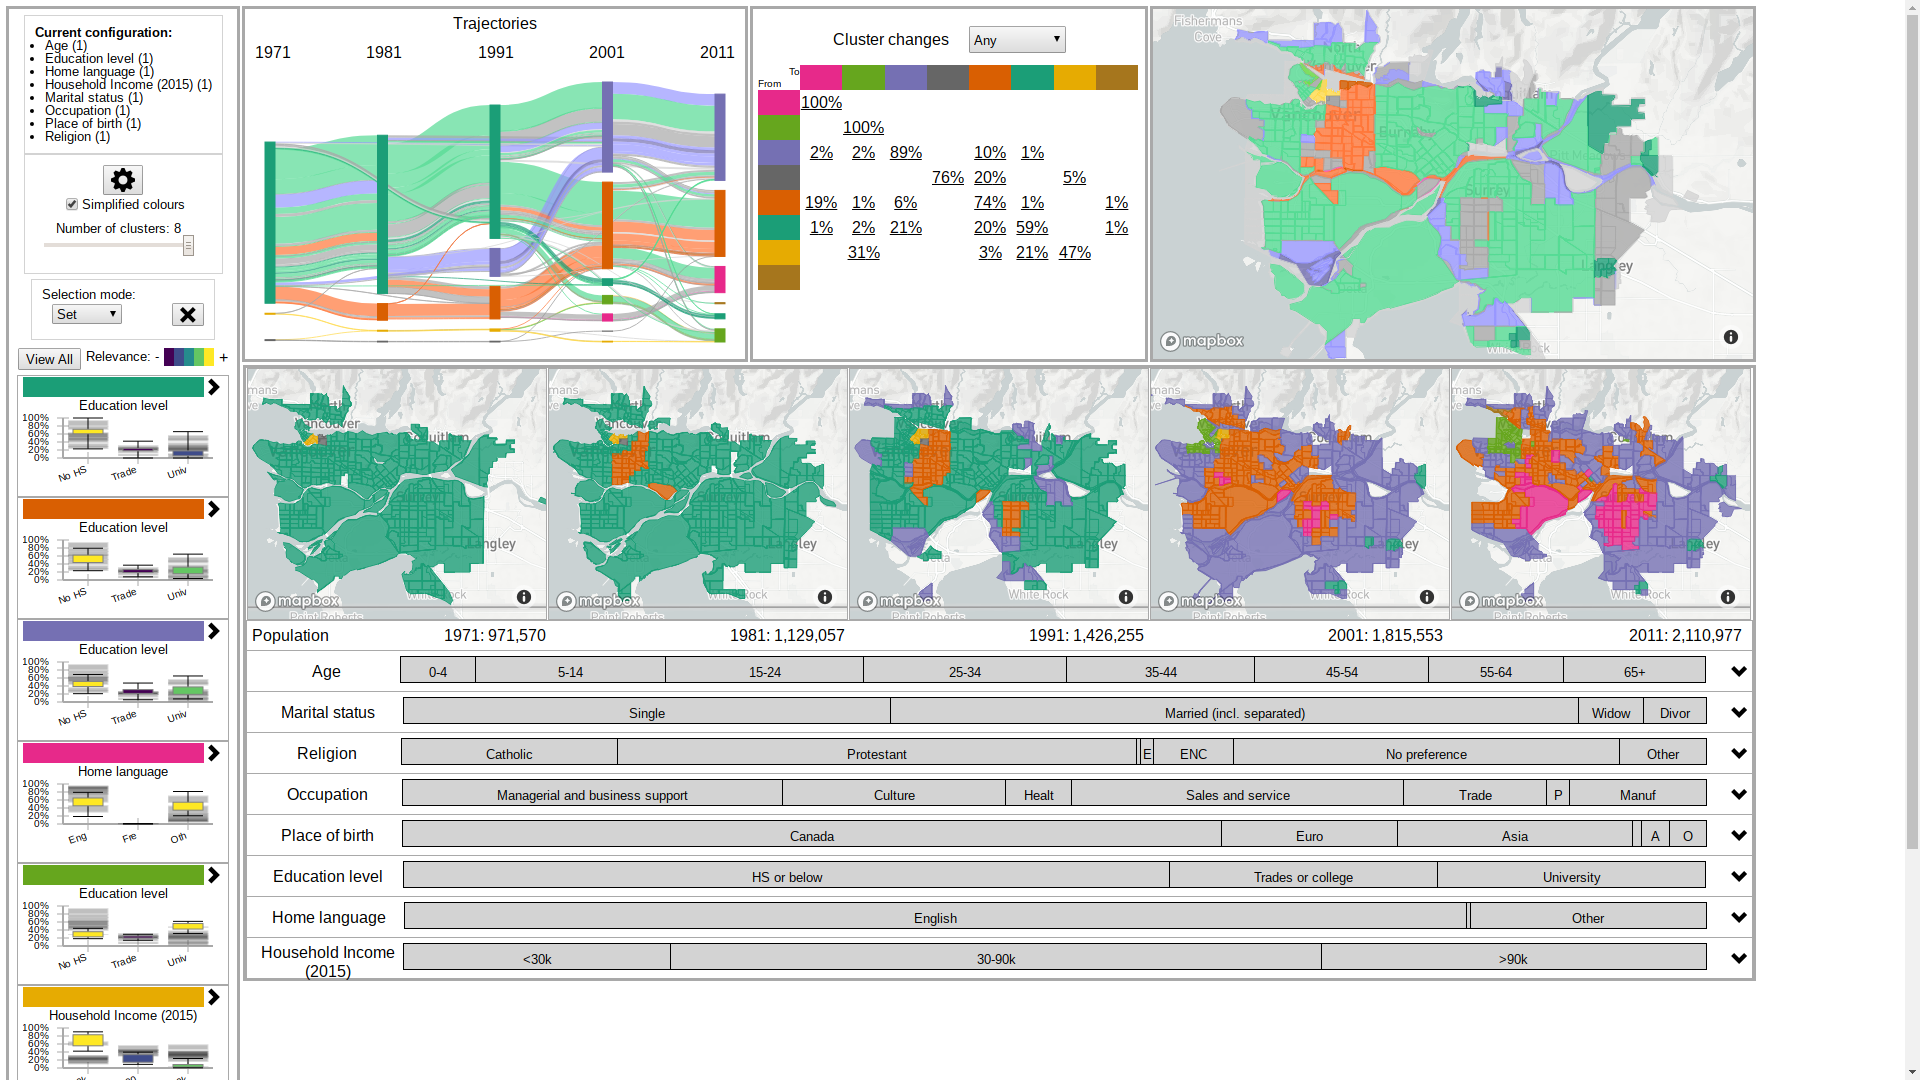
\includegraphics[width=\linewidth]{39a.png}
    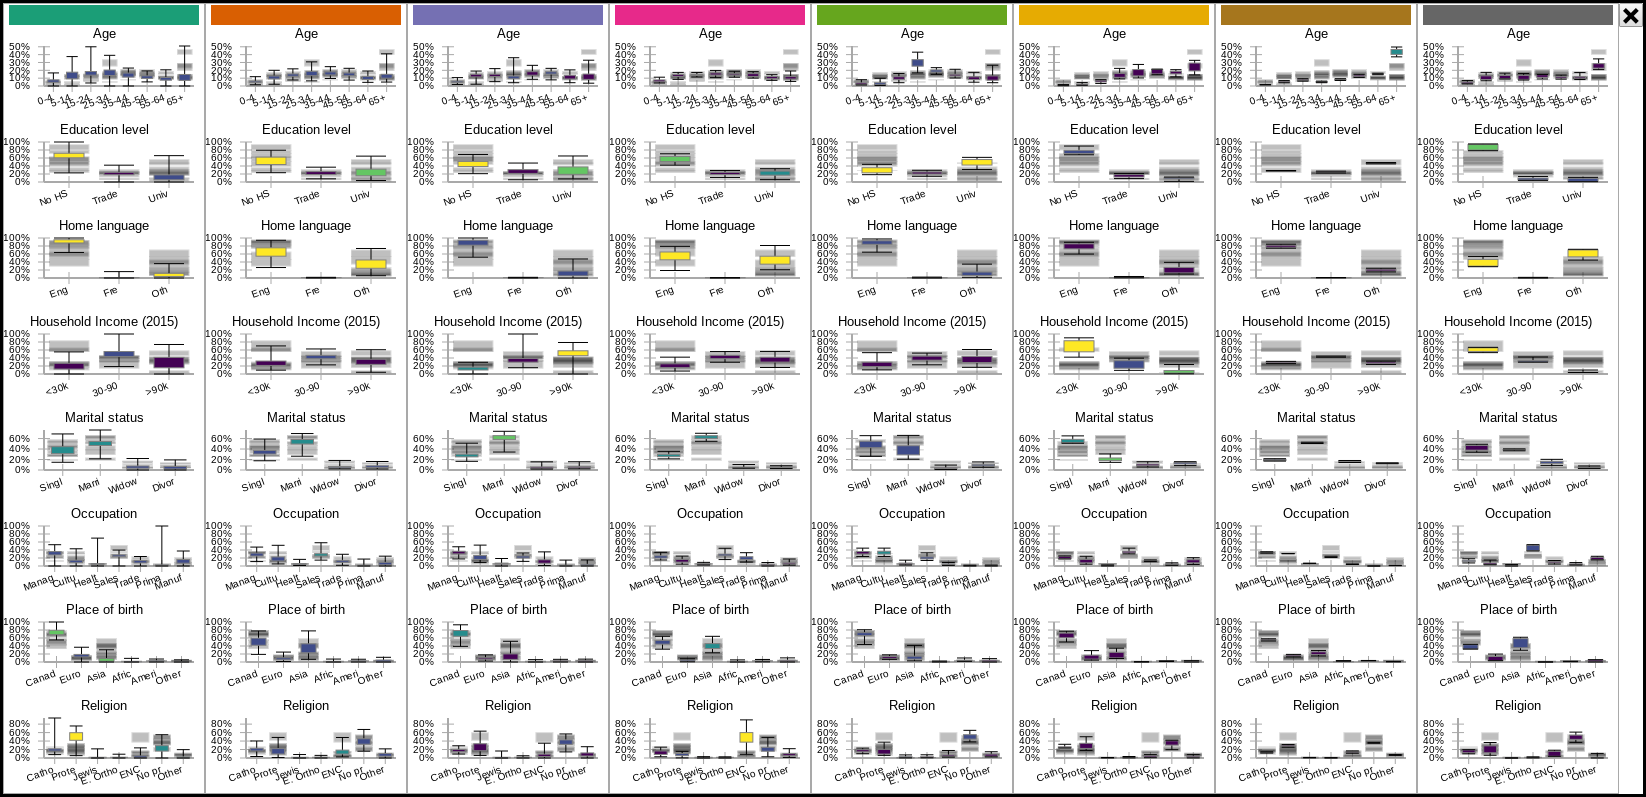
\includegraphics[width=\linewidth]{39b.png}
\end{center}

\subsection{Toronto}
\begin{center}
    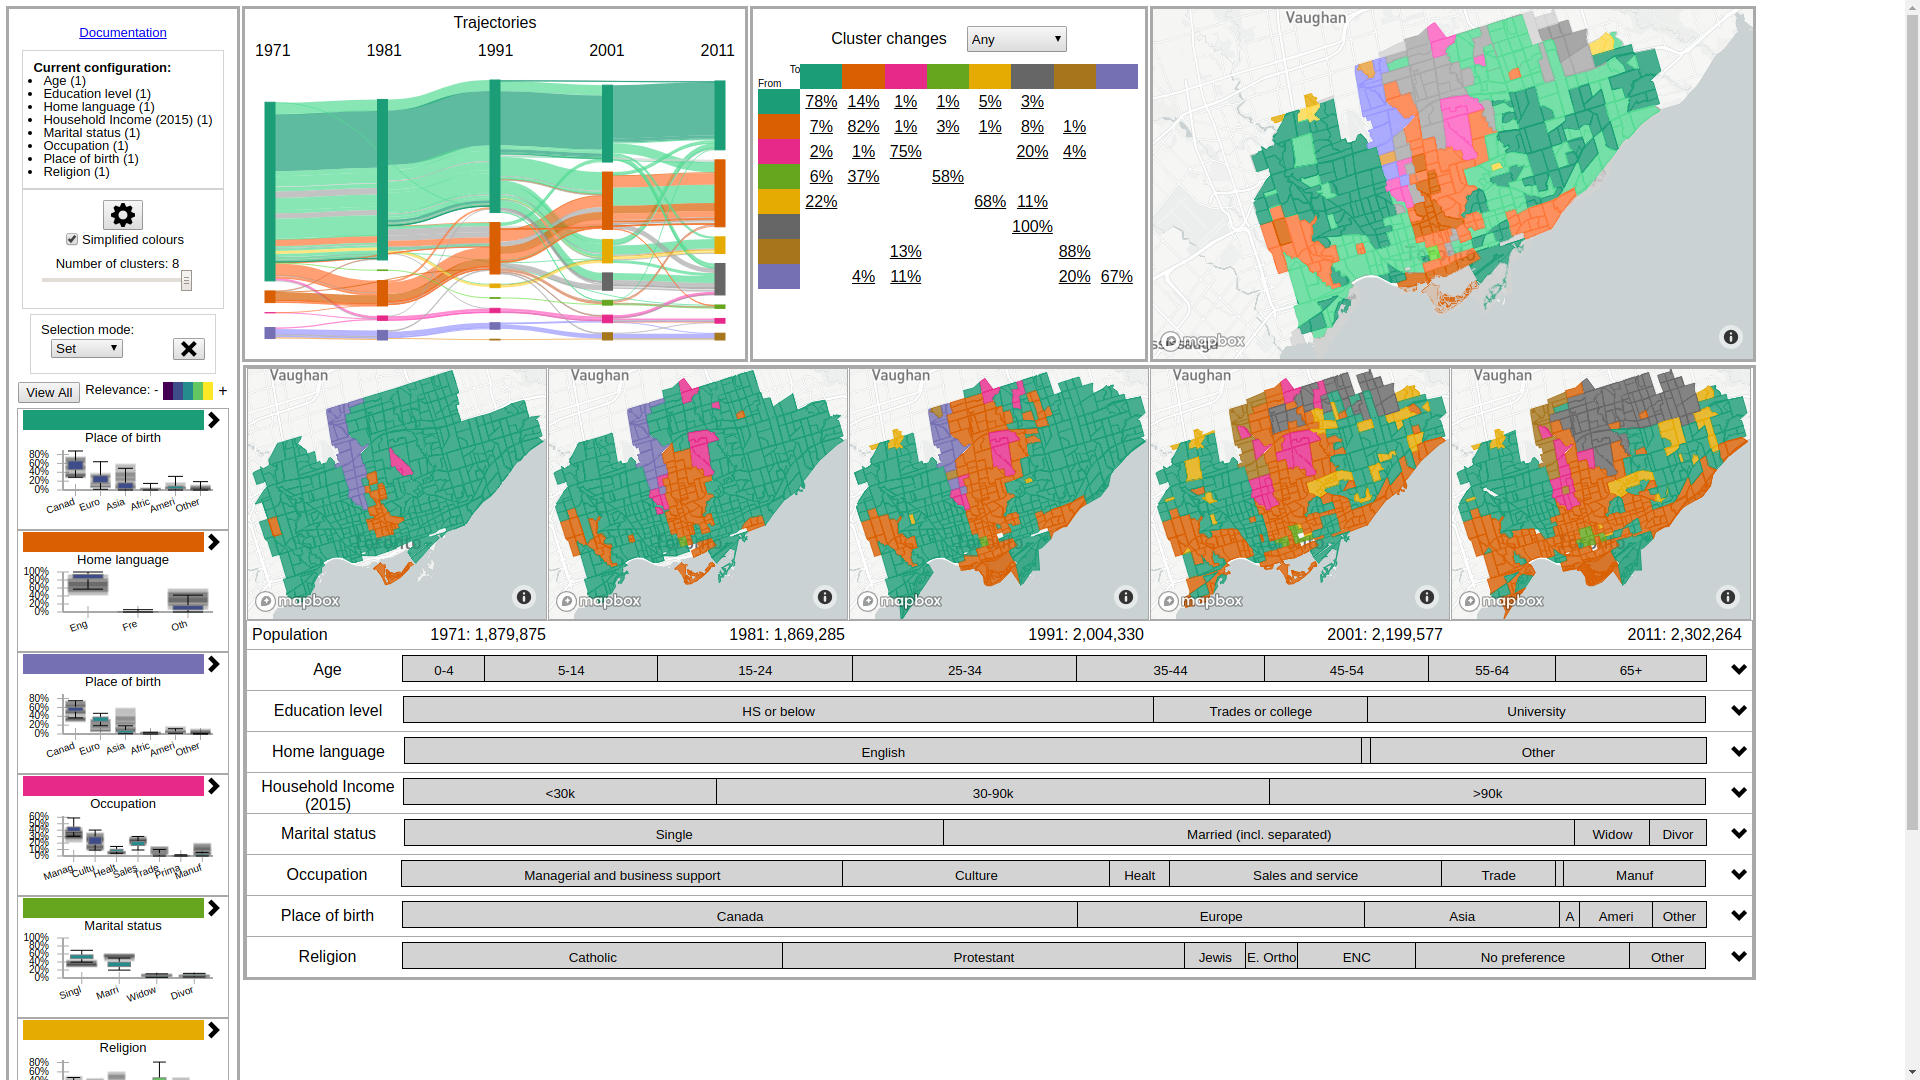
\includegraphics[width=\linewidth]{40a.png}
    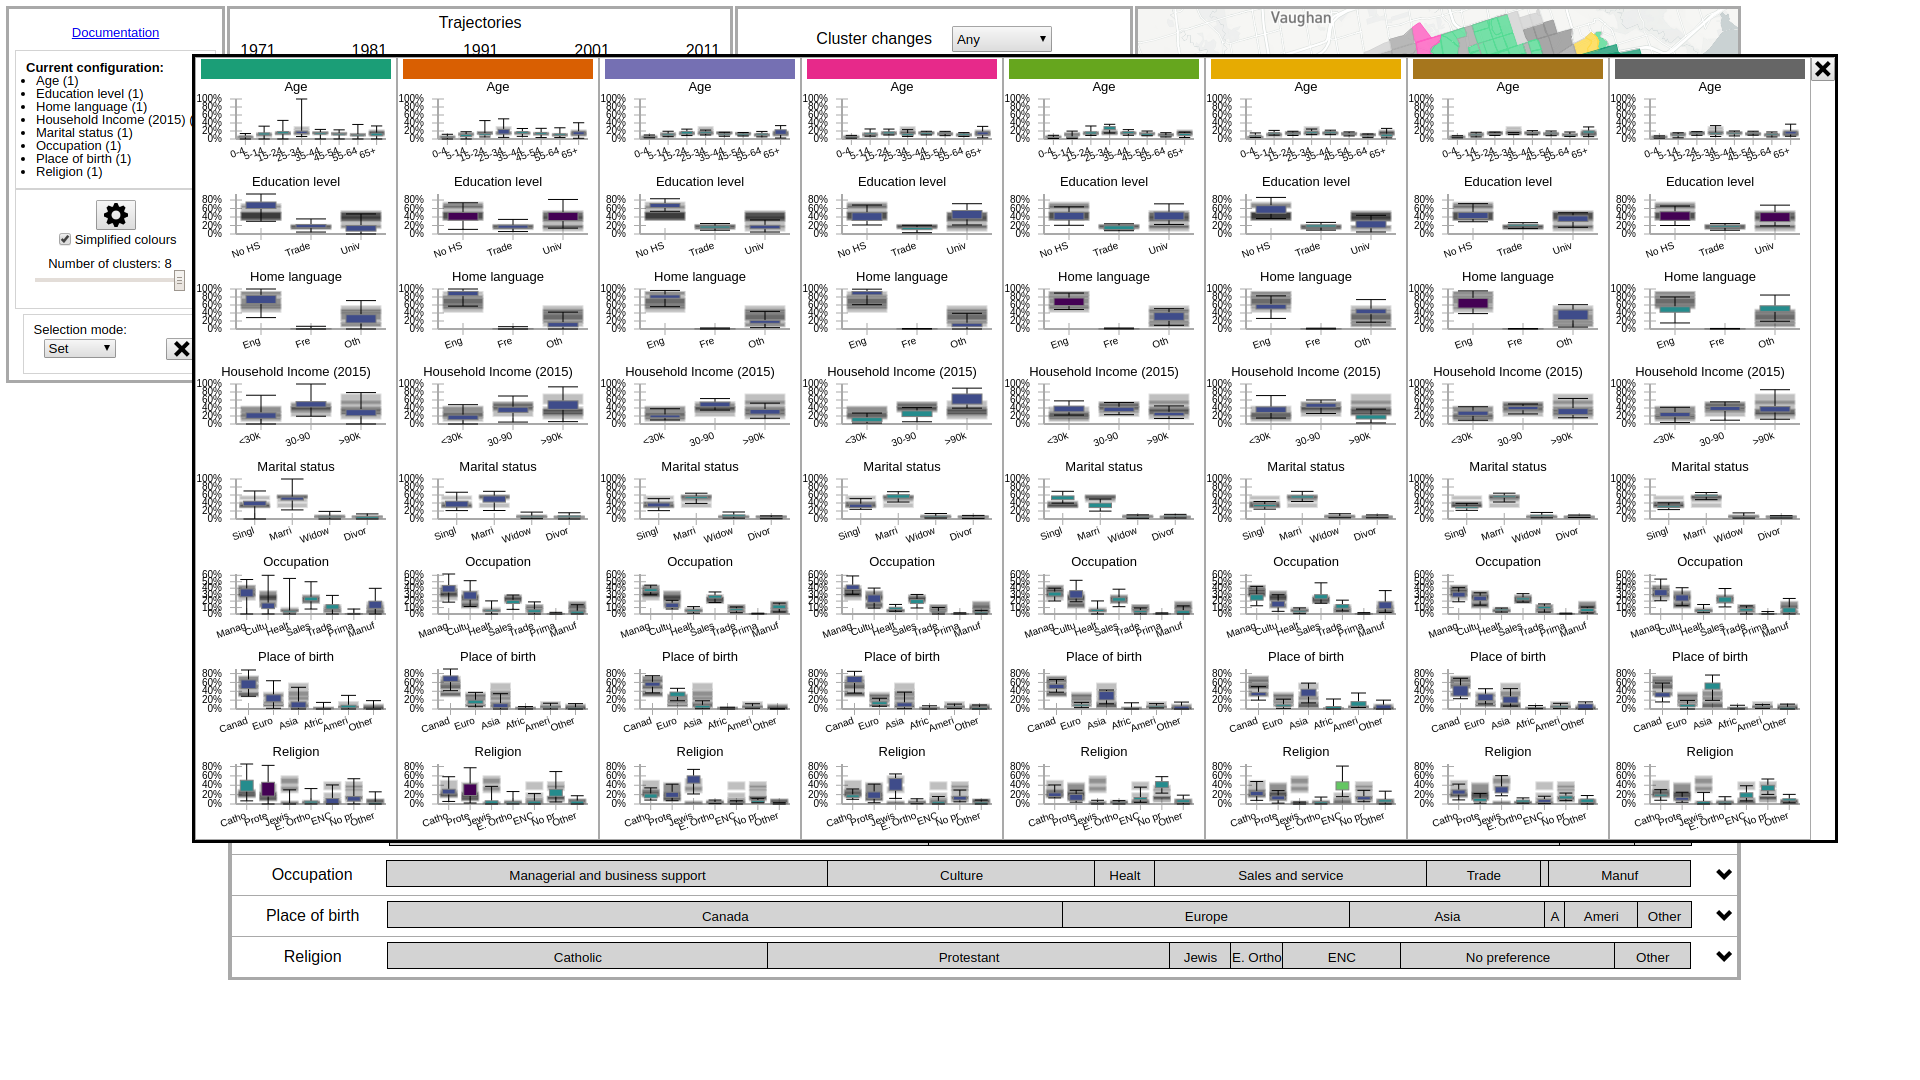
\includegraphics[width=\linewidth]{40b.png}
\end{center}

\subsection{Montreal}
\begin{center}
    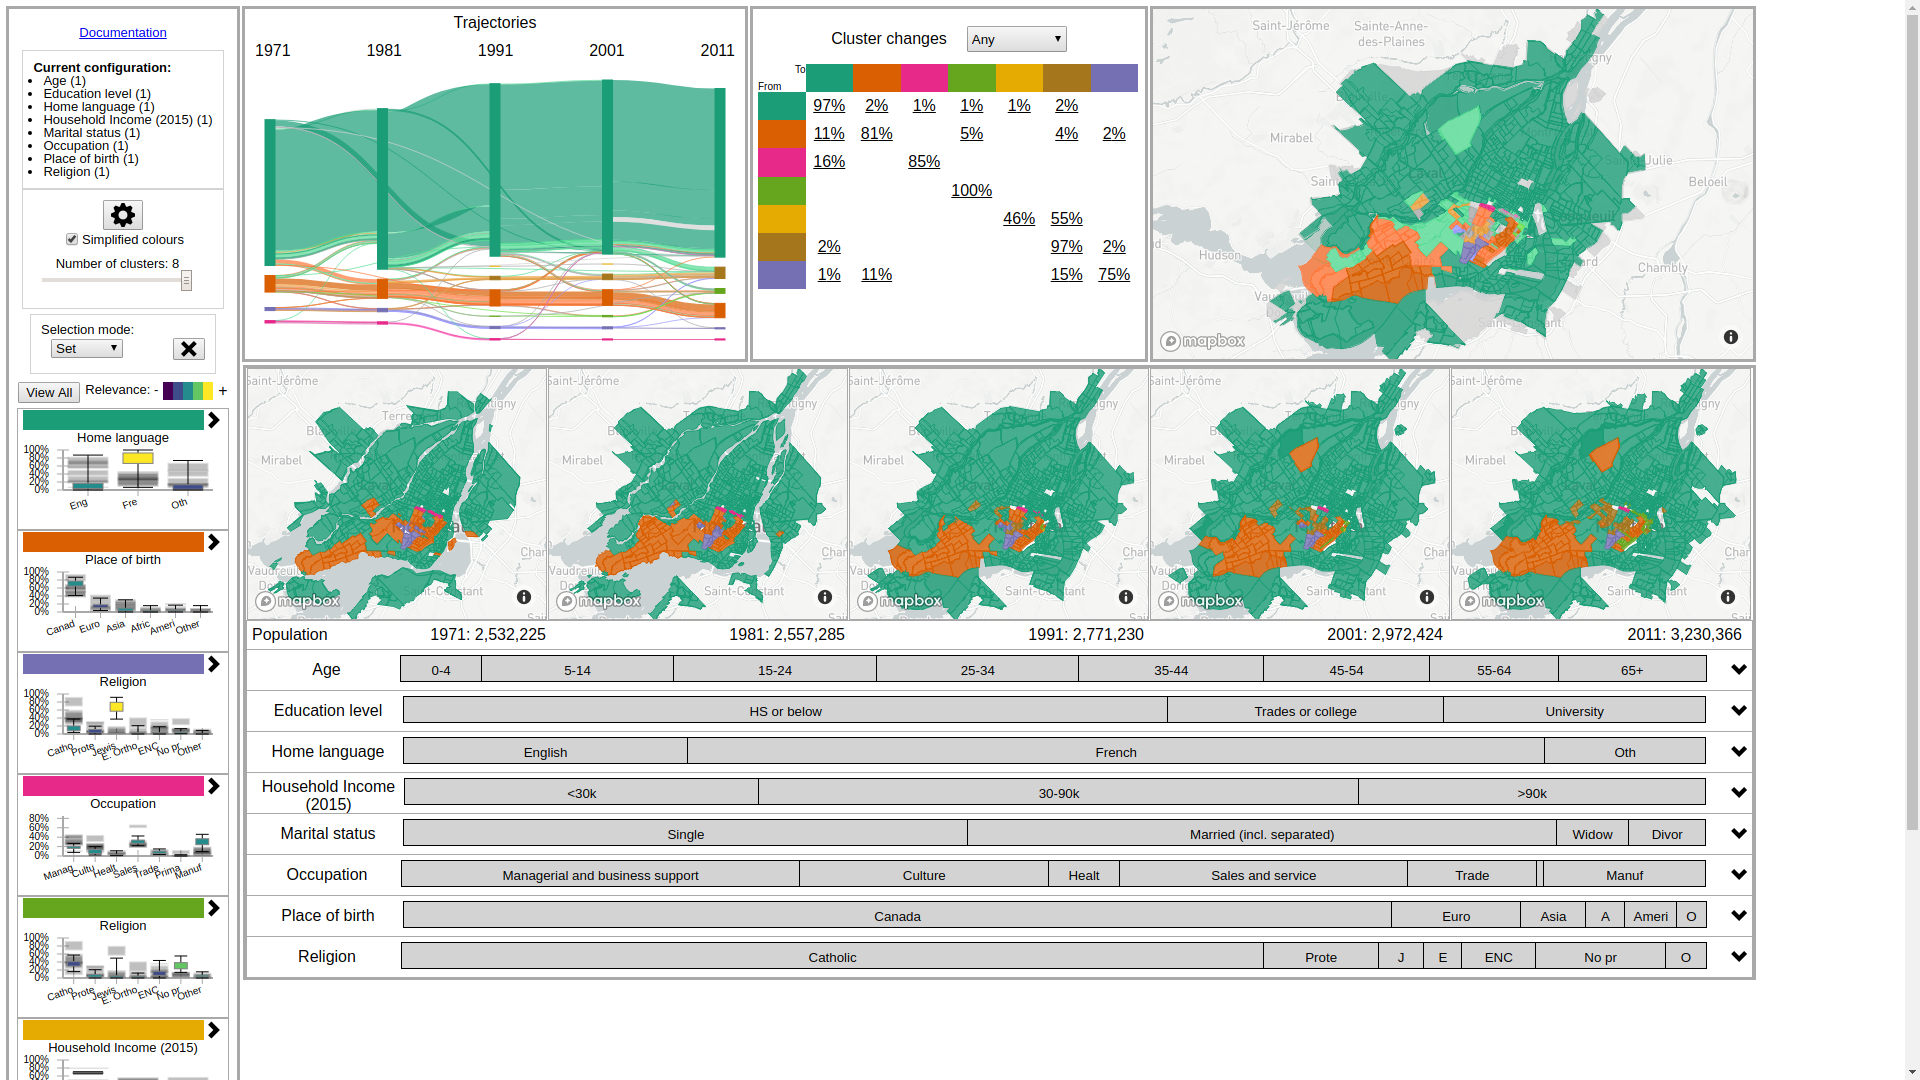
\includegraphics[width=\linewidth]{41a.png}
    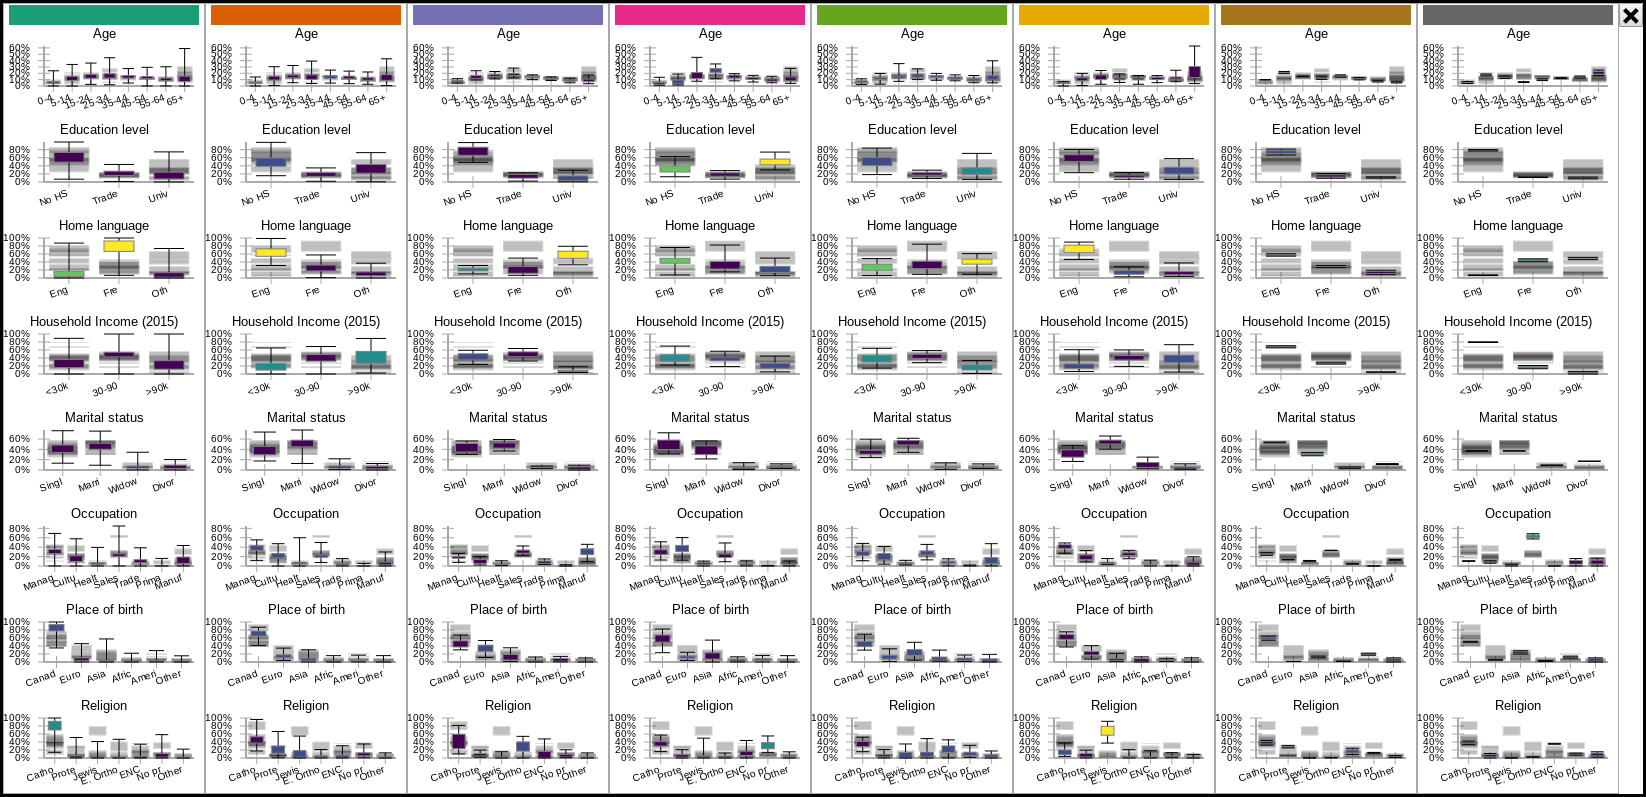
\includegraphics[width=\linewidth]{41b.png}
\end{center}

\subsection{Calgary}
\begin{center}
	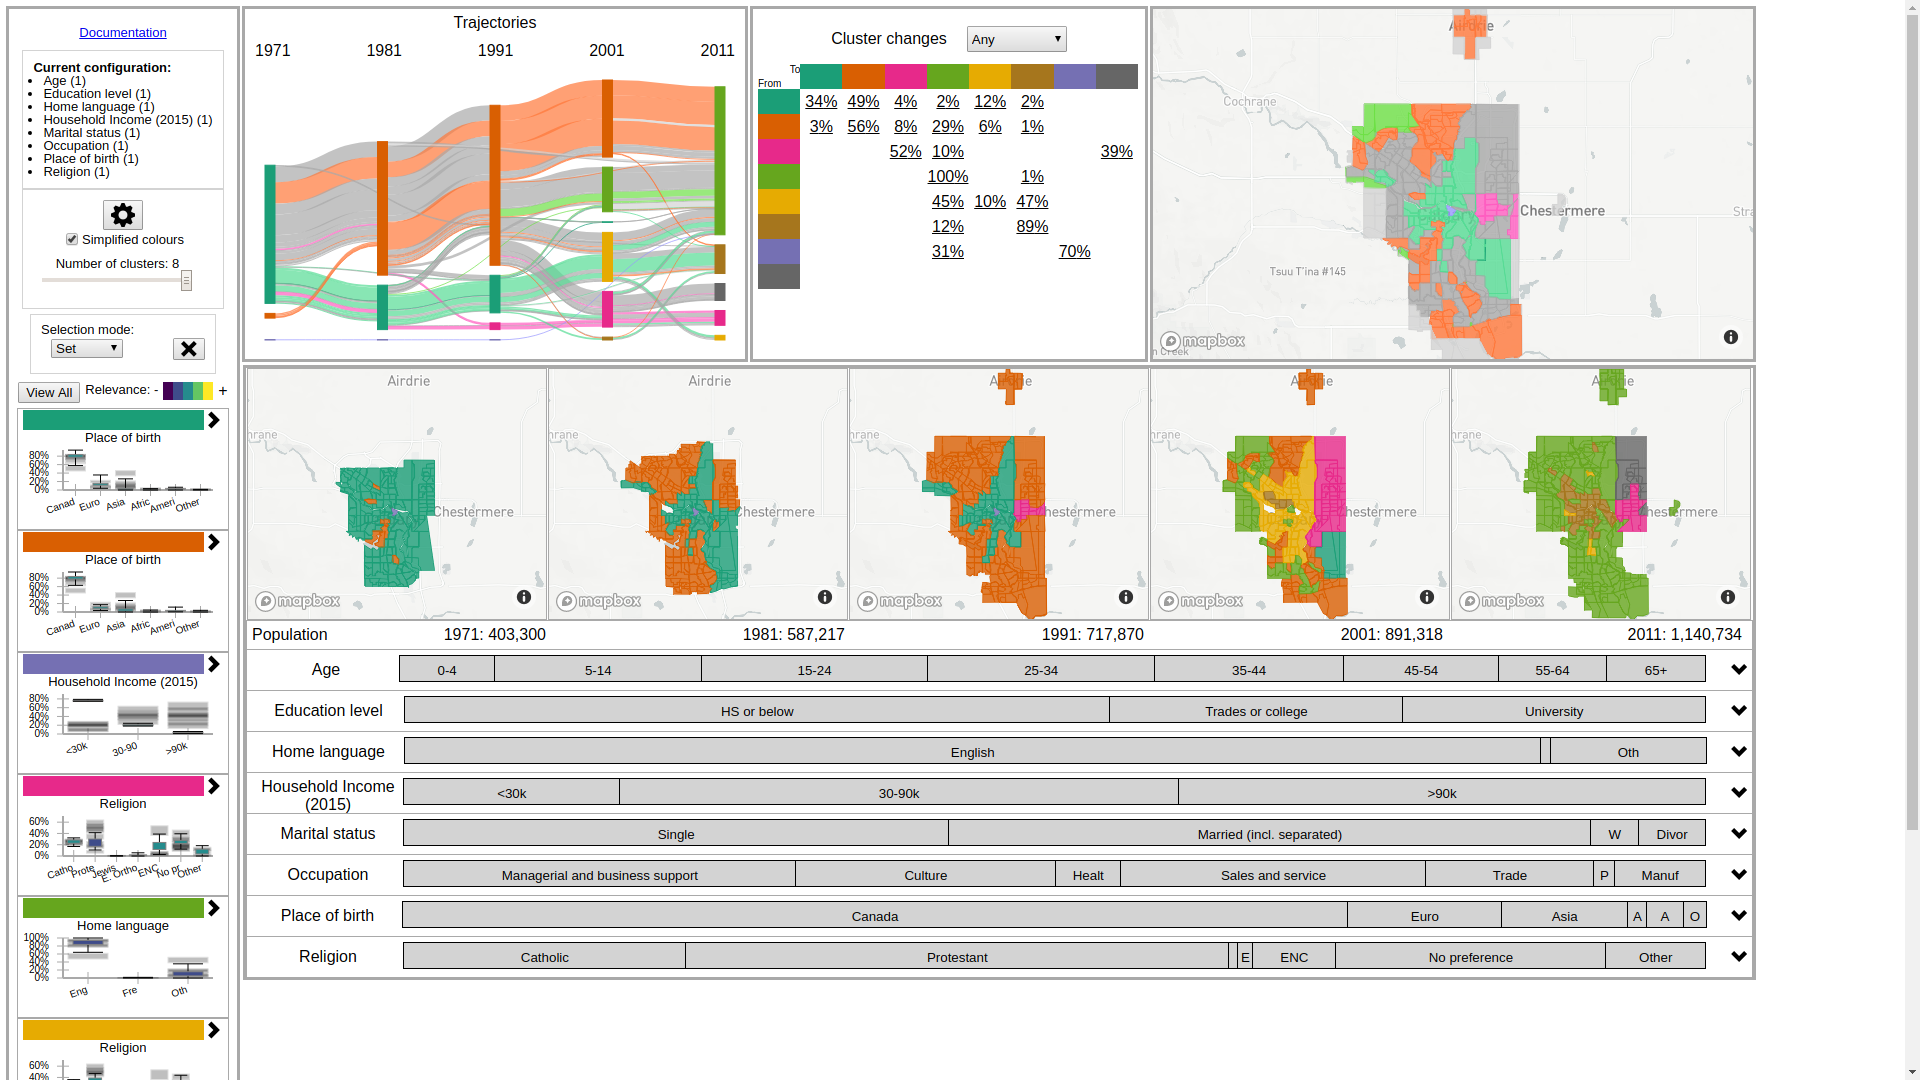
\includegraphics[width=\linewidth]{1a.png}
	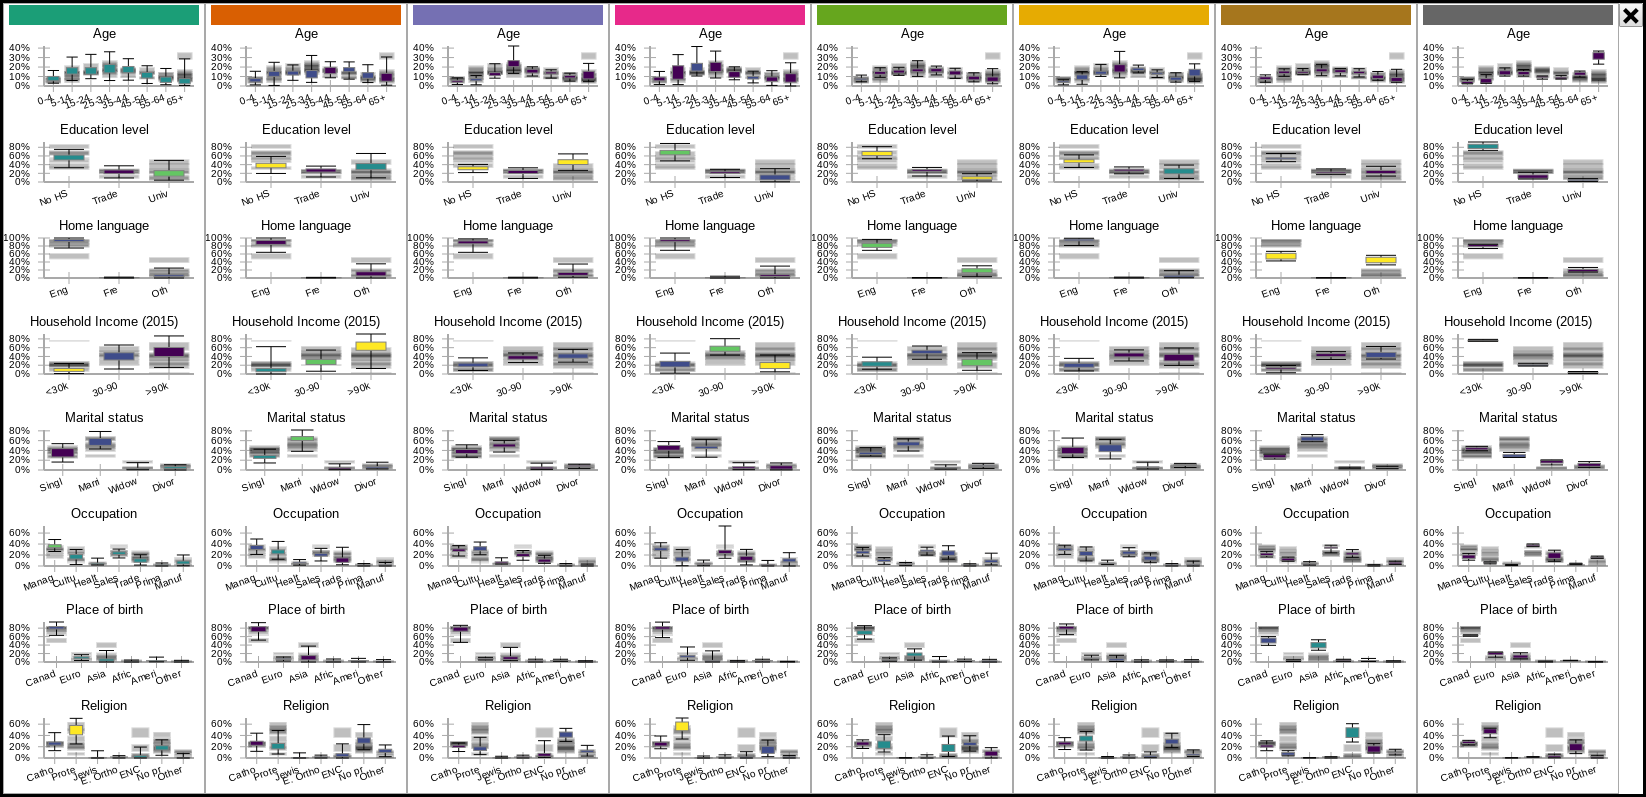
\includegraphics[width=\linewidth]{1b.png}
\end{center}



\subsection{Edmonton}
\begin{center}
	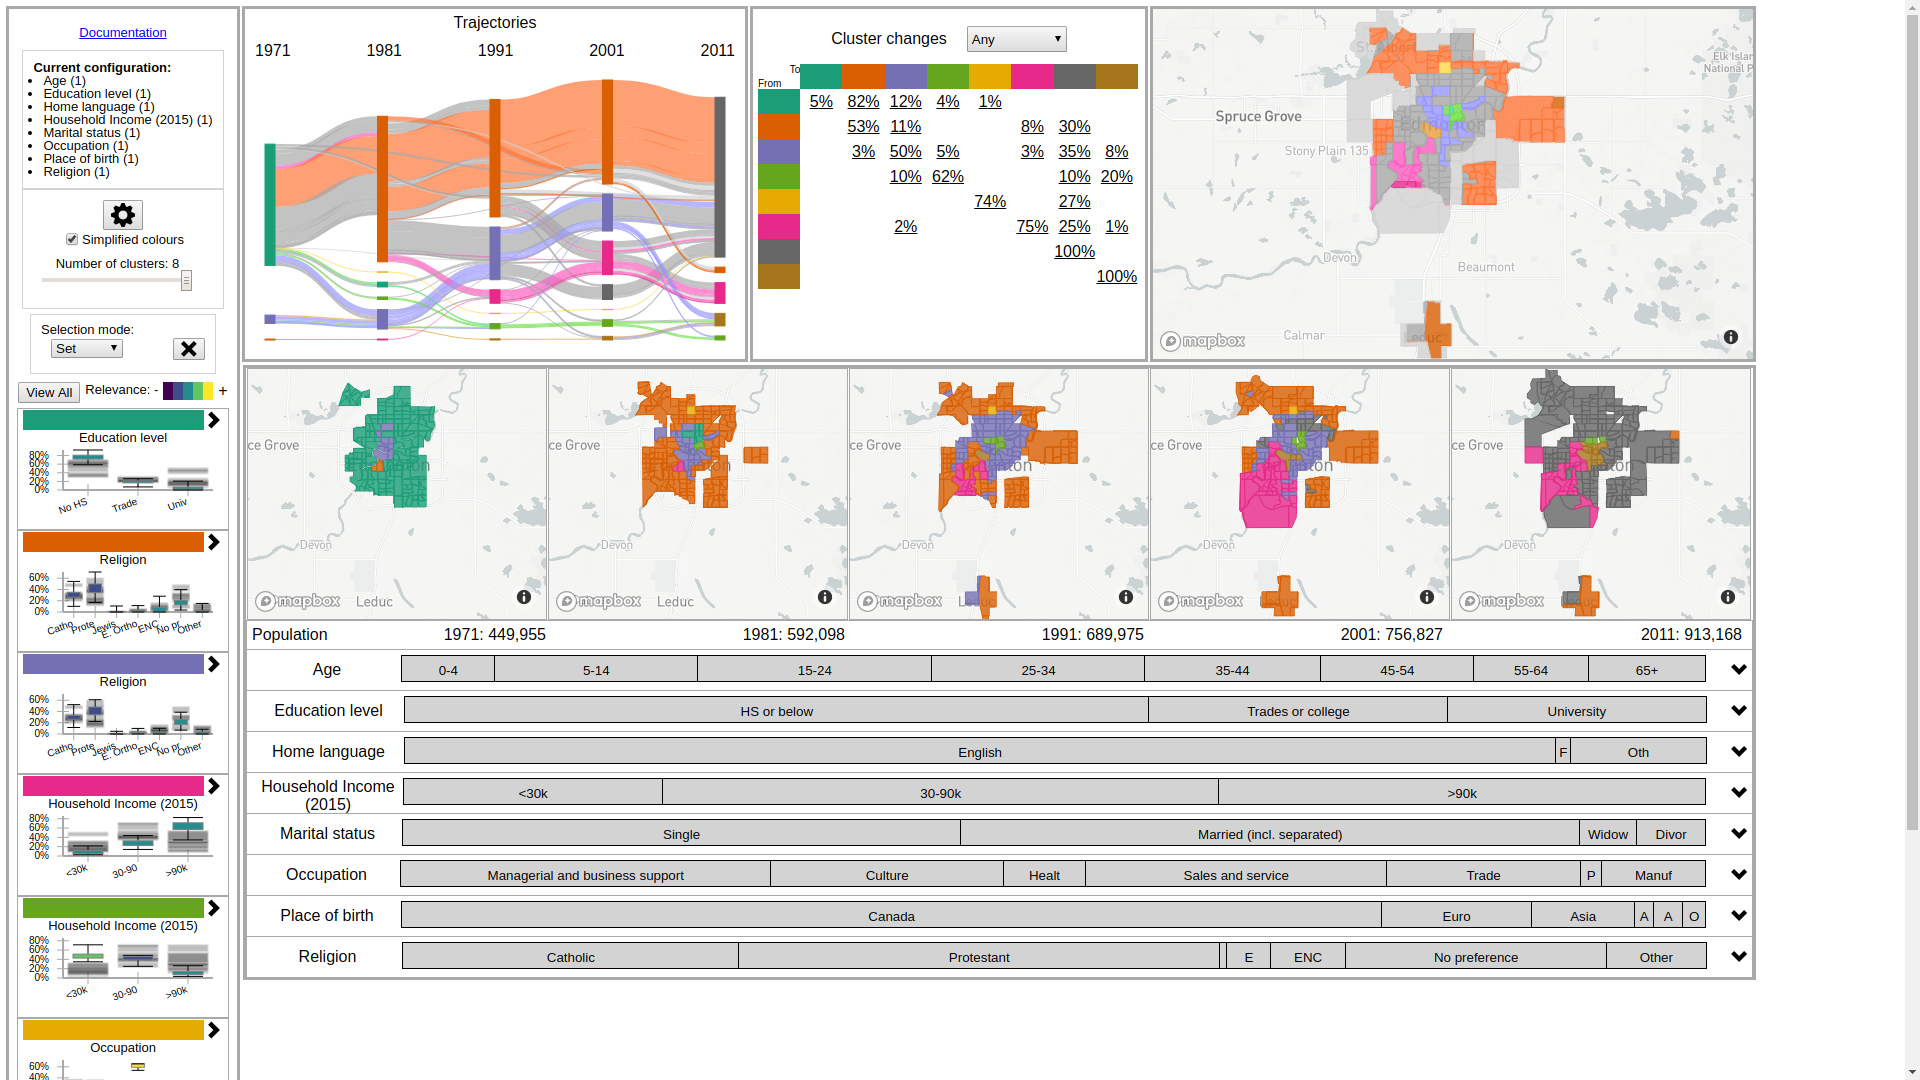
\includegraphics[width=\linewidth]{2a.png}
	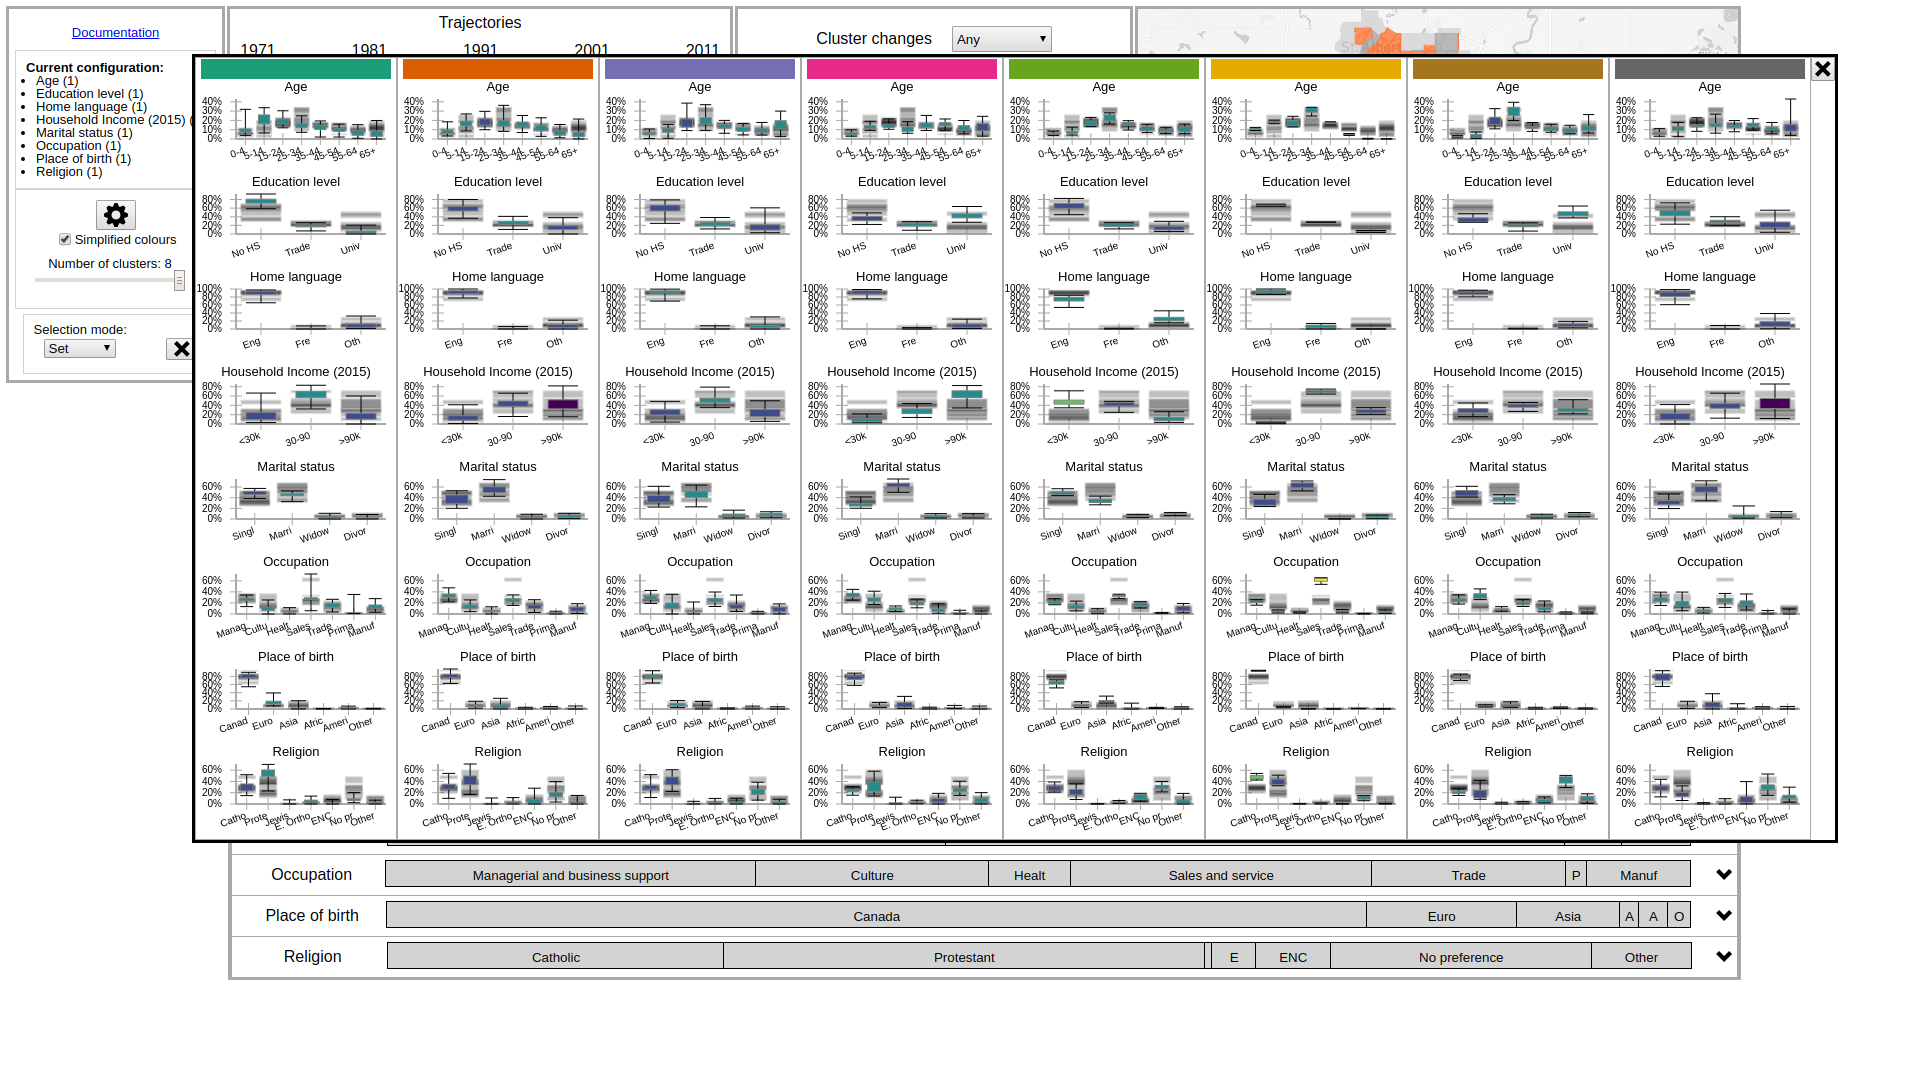
\includegraphics[width=\linewidth]{2b.png}
\end{center}



\subsection{Halifax}
\begin{center}
	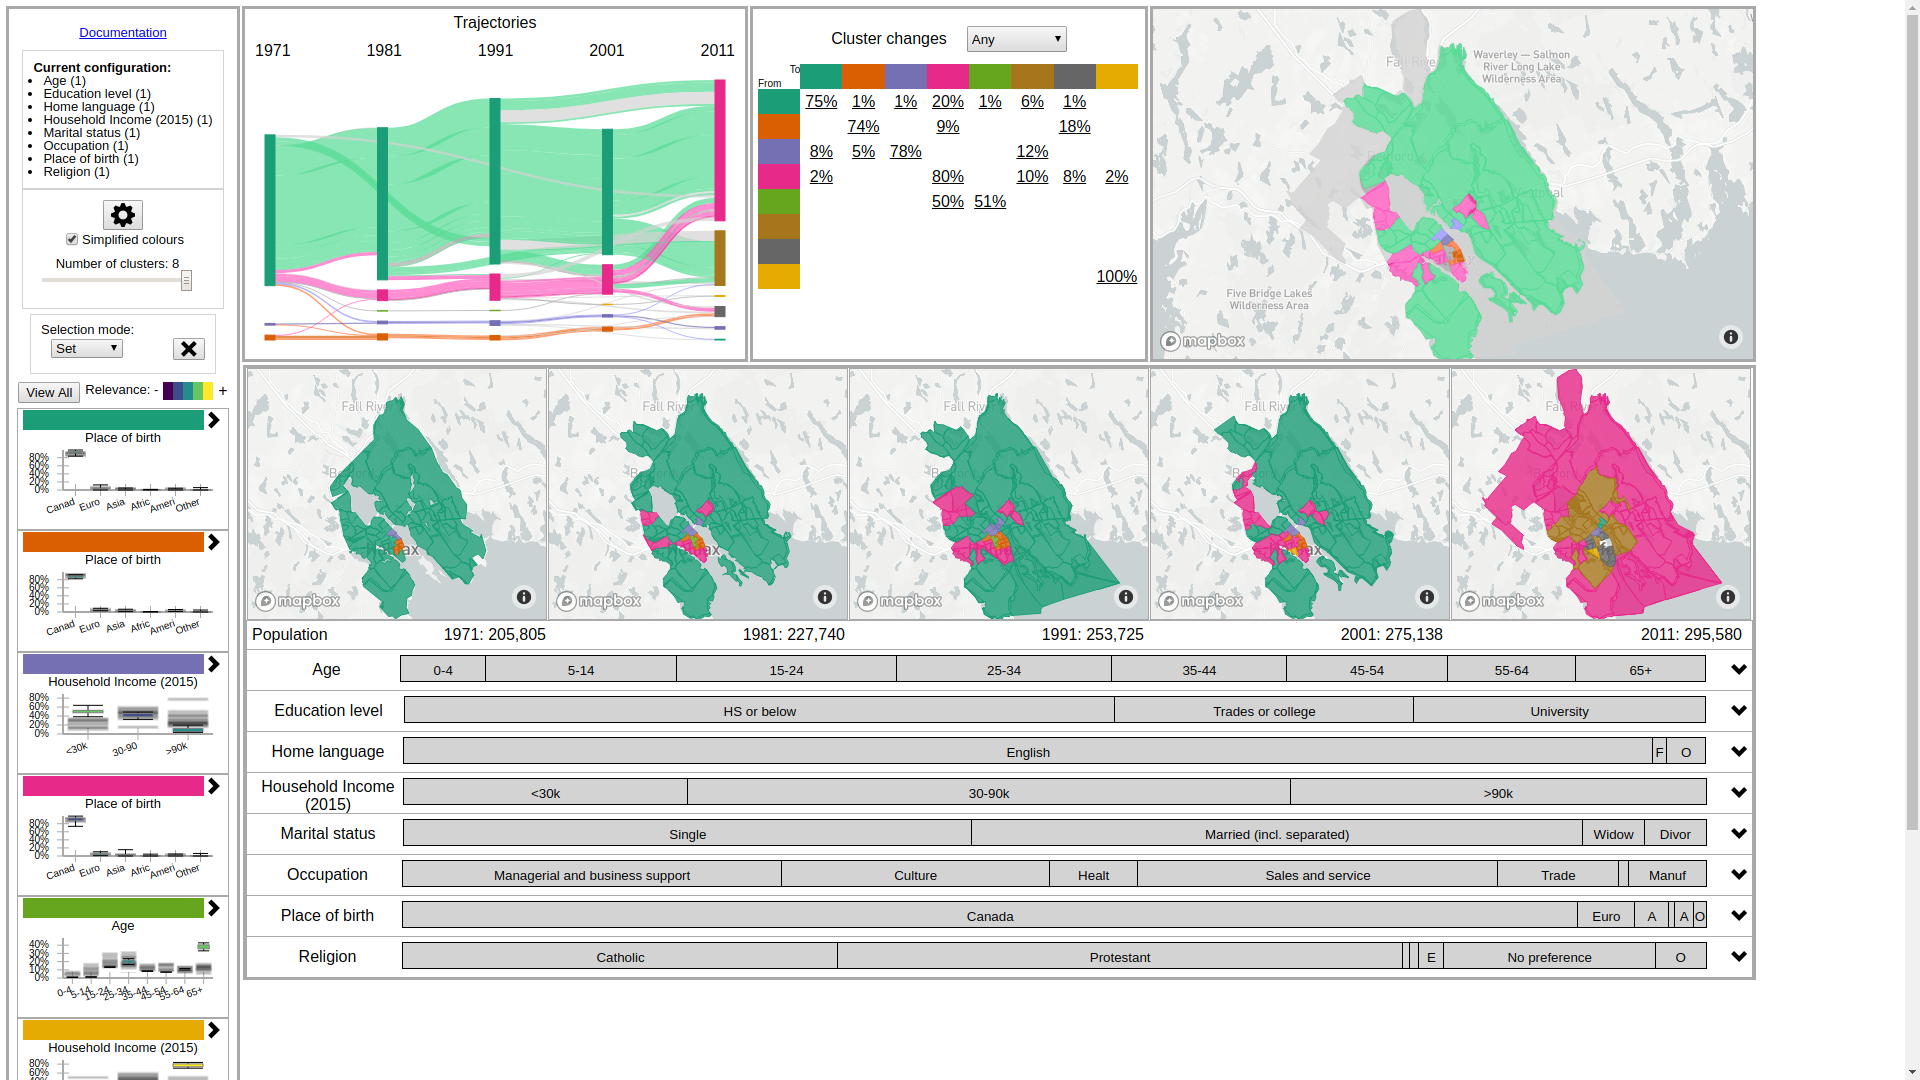
\includegraphics[width=\linewidth]{3a.png}
	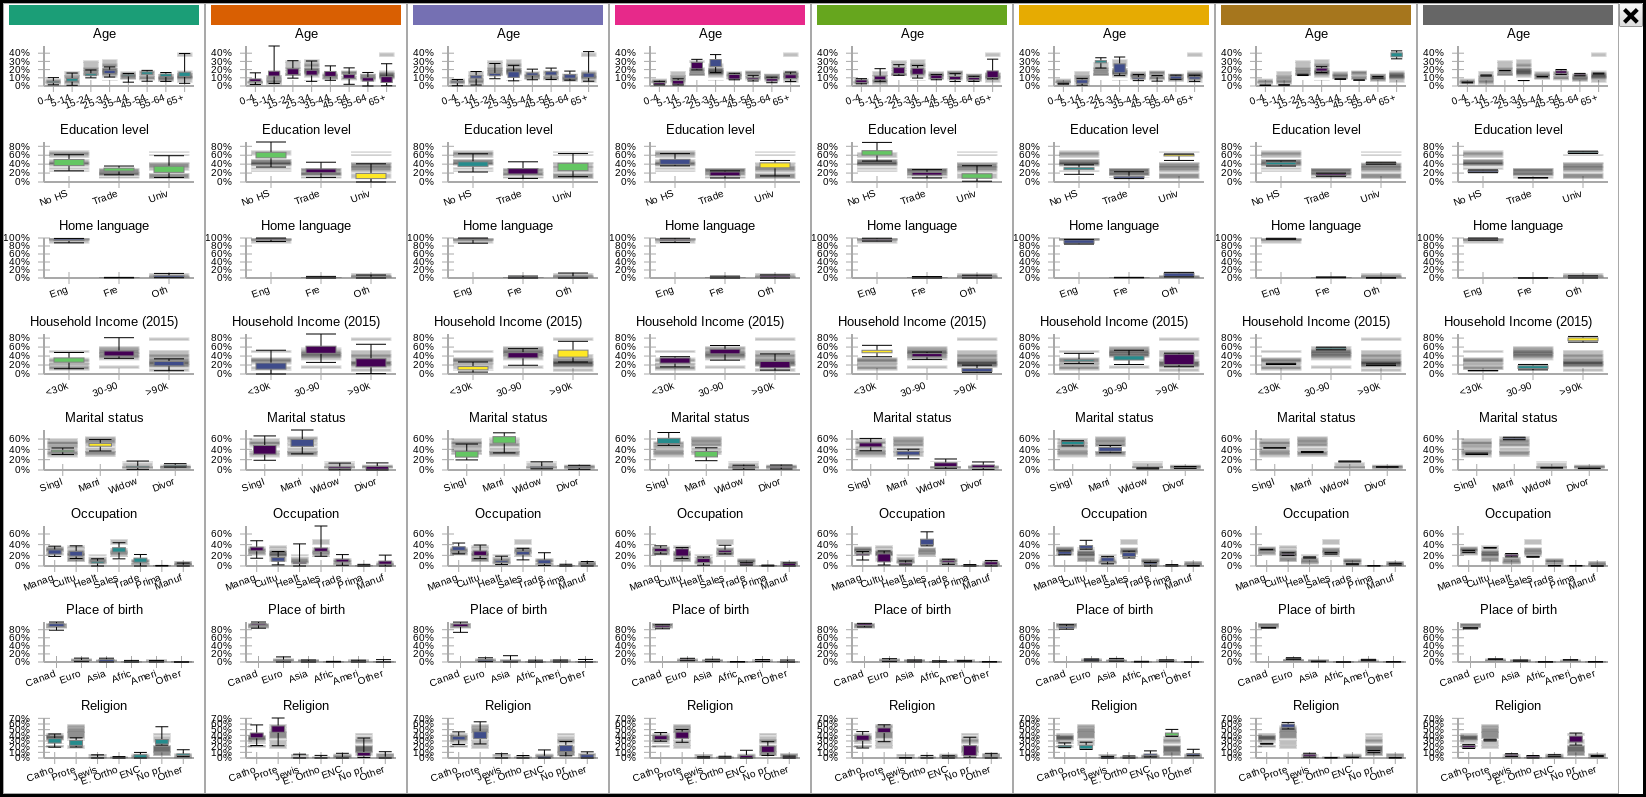
\includegraphics[width=\linewidth]{3b.png}
\end{center}



\subsection{Ottawa}
\begin{center}
	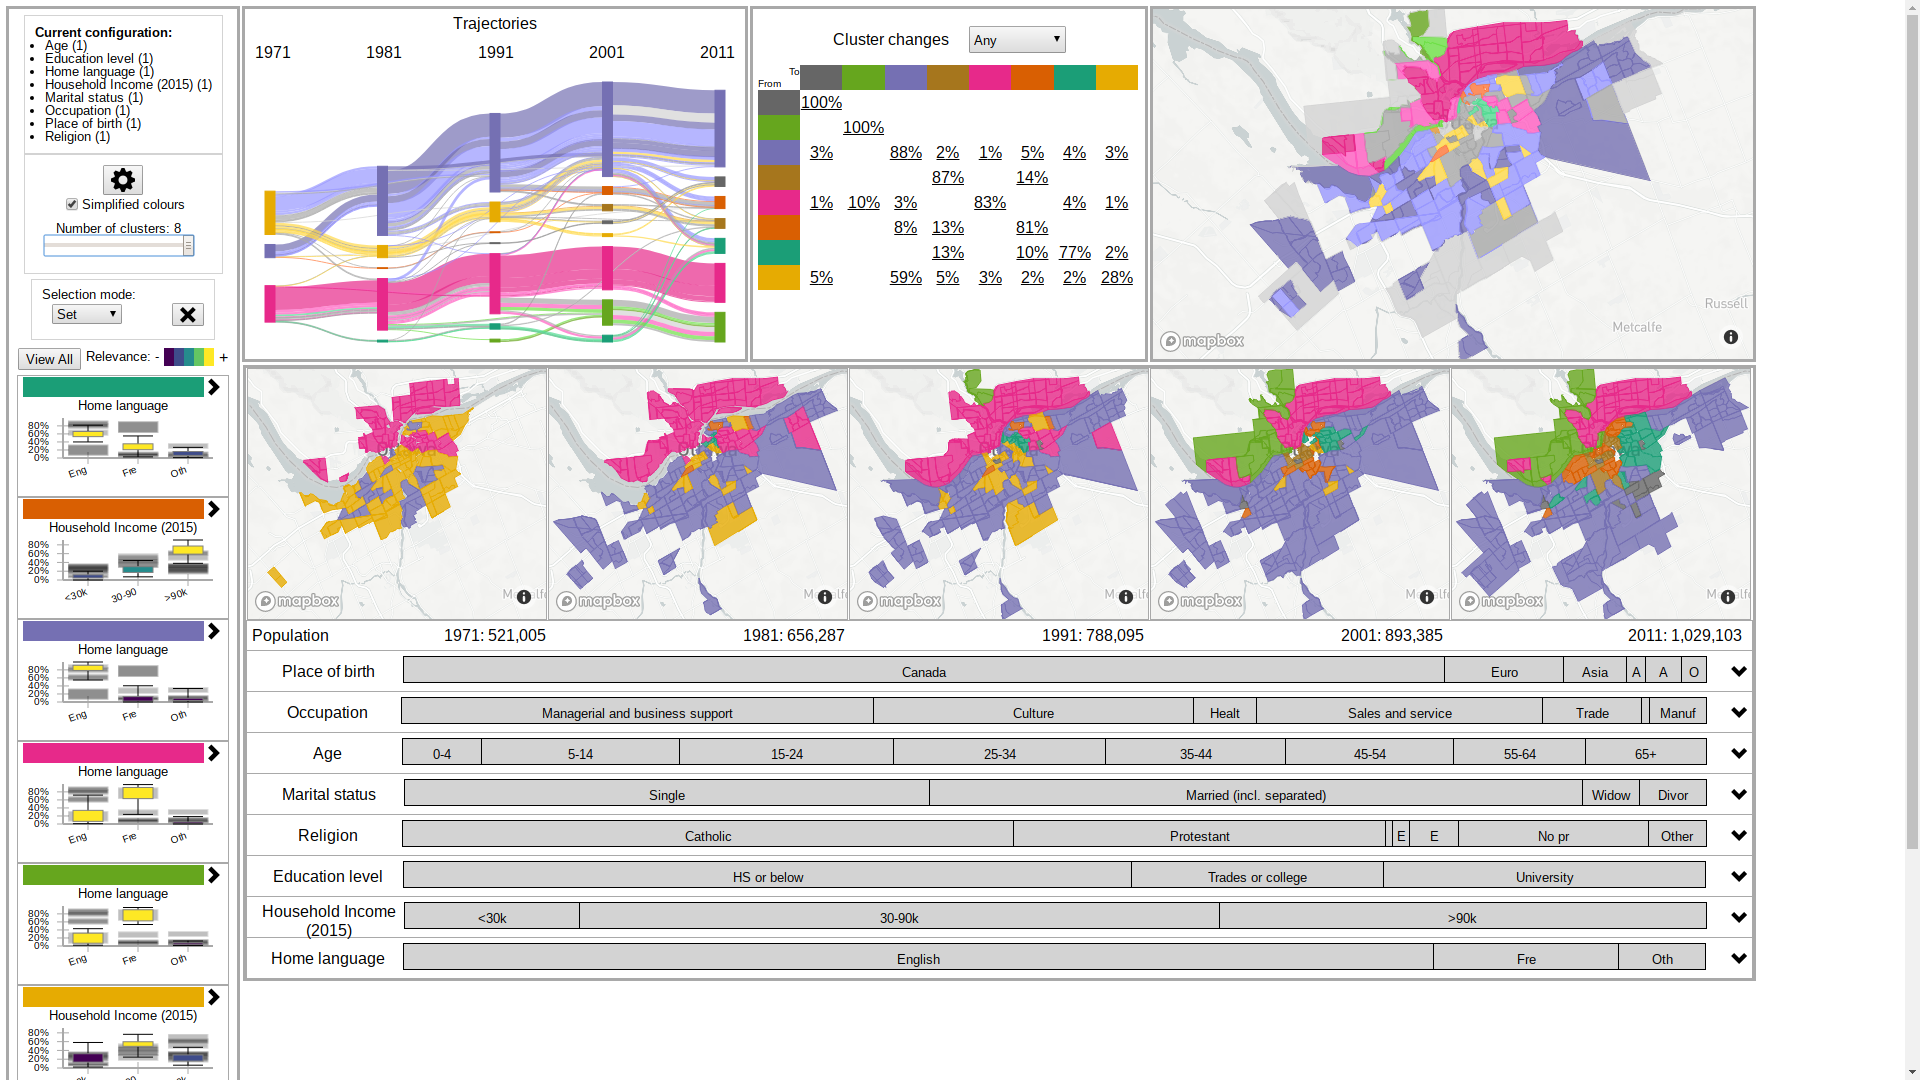
\includegraphics[width=\linewidth]{4a.png}
	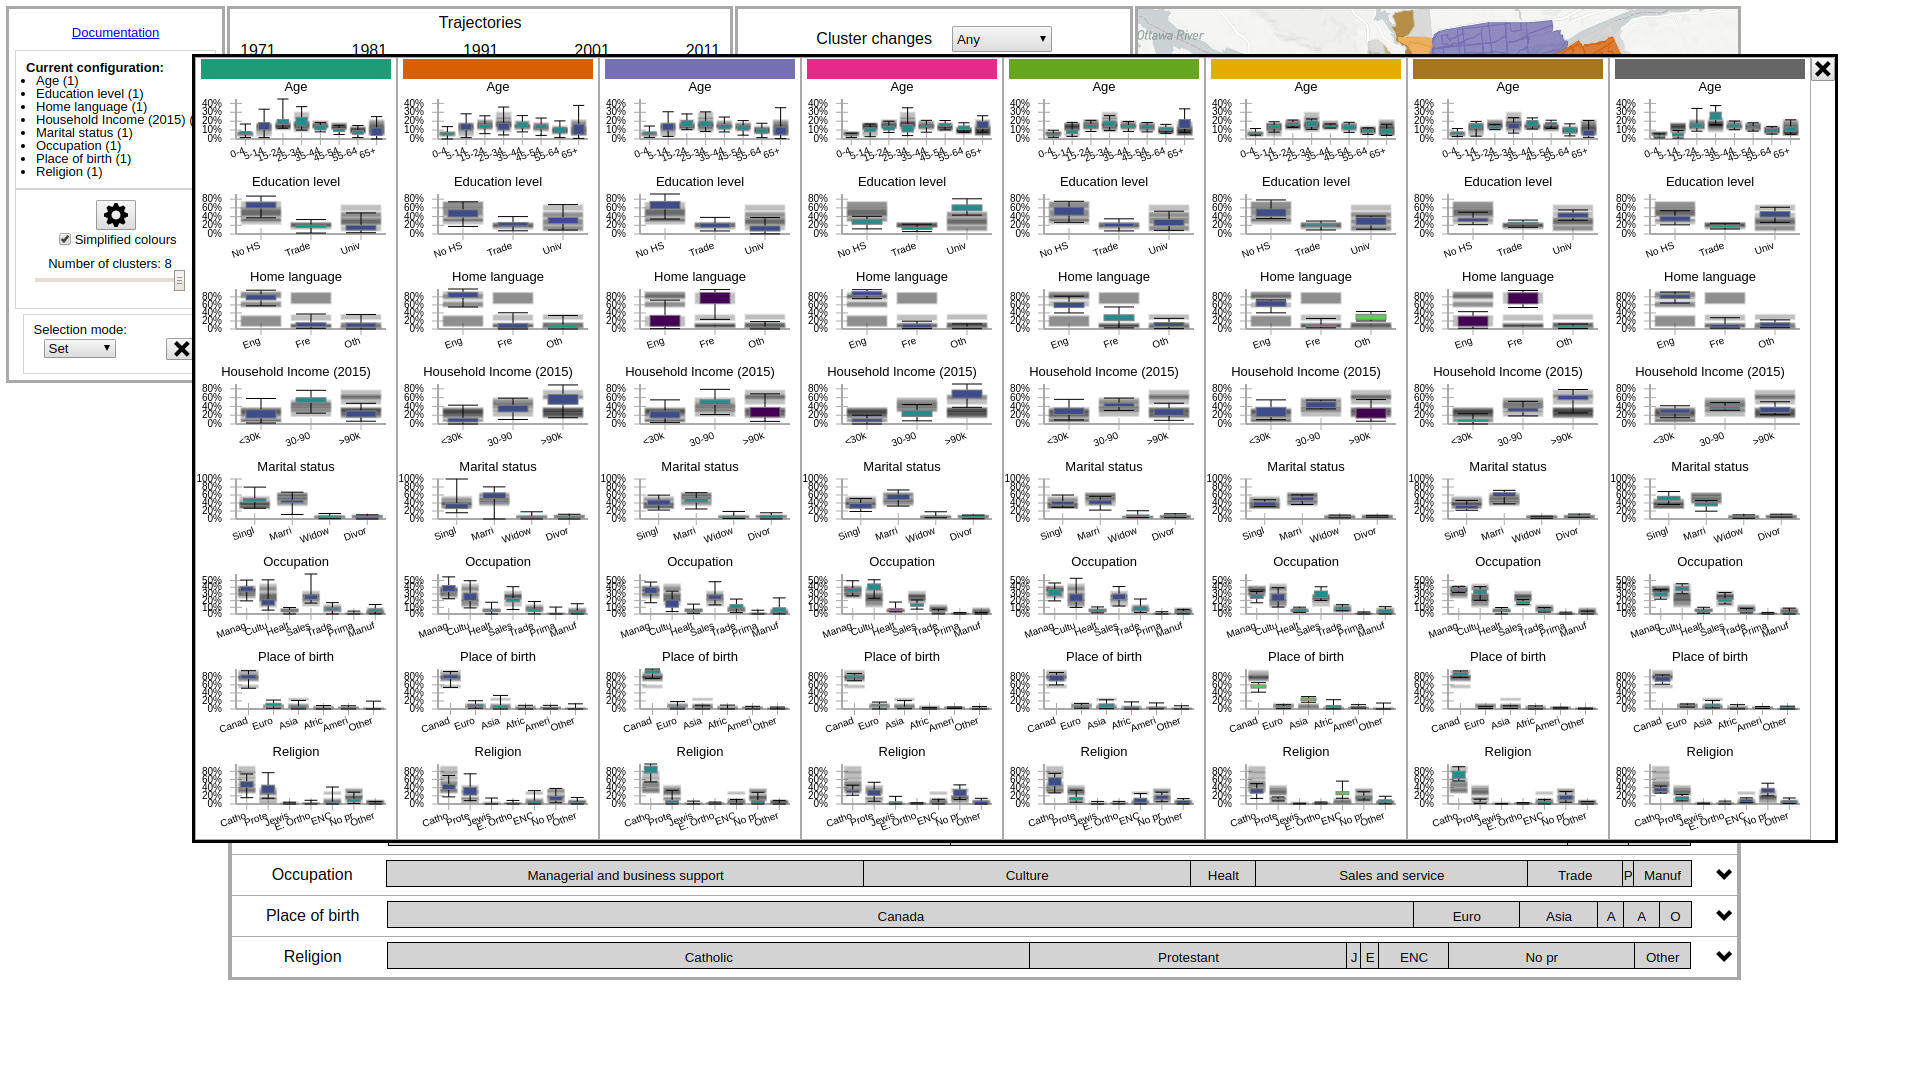
\includegraphics[width=\linewidth]{4b.png}
\end{center}



\subsection{Quebec City}
\begin{center}
	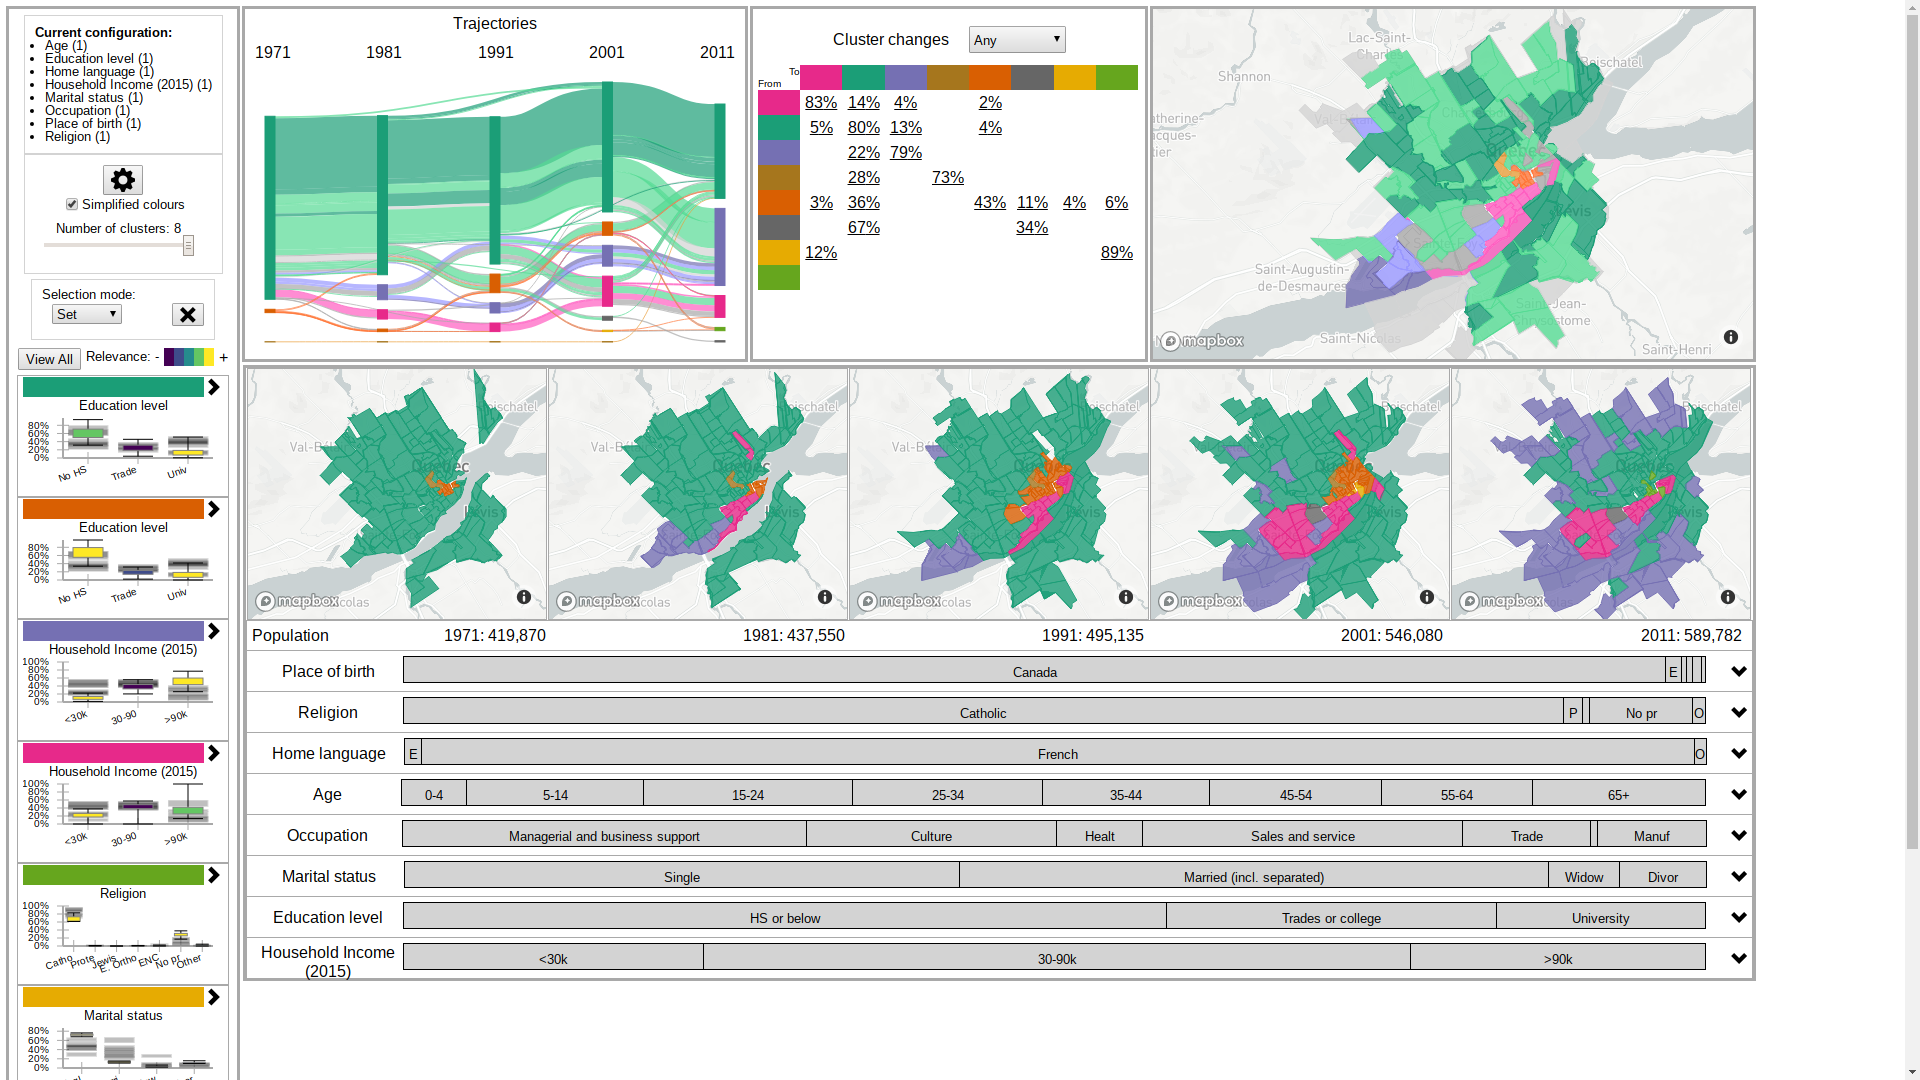
\includegraphics[width=\linewidth]{5a.png}
	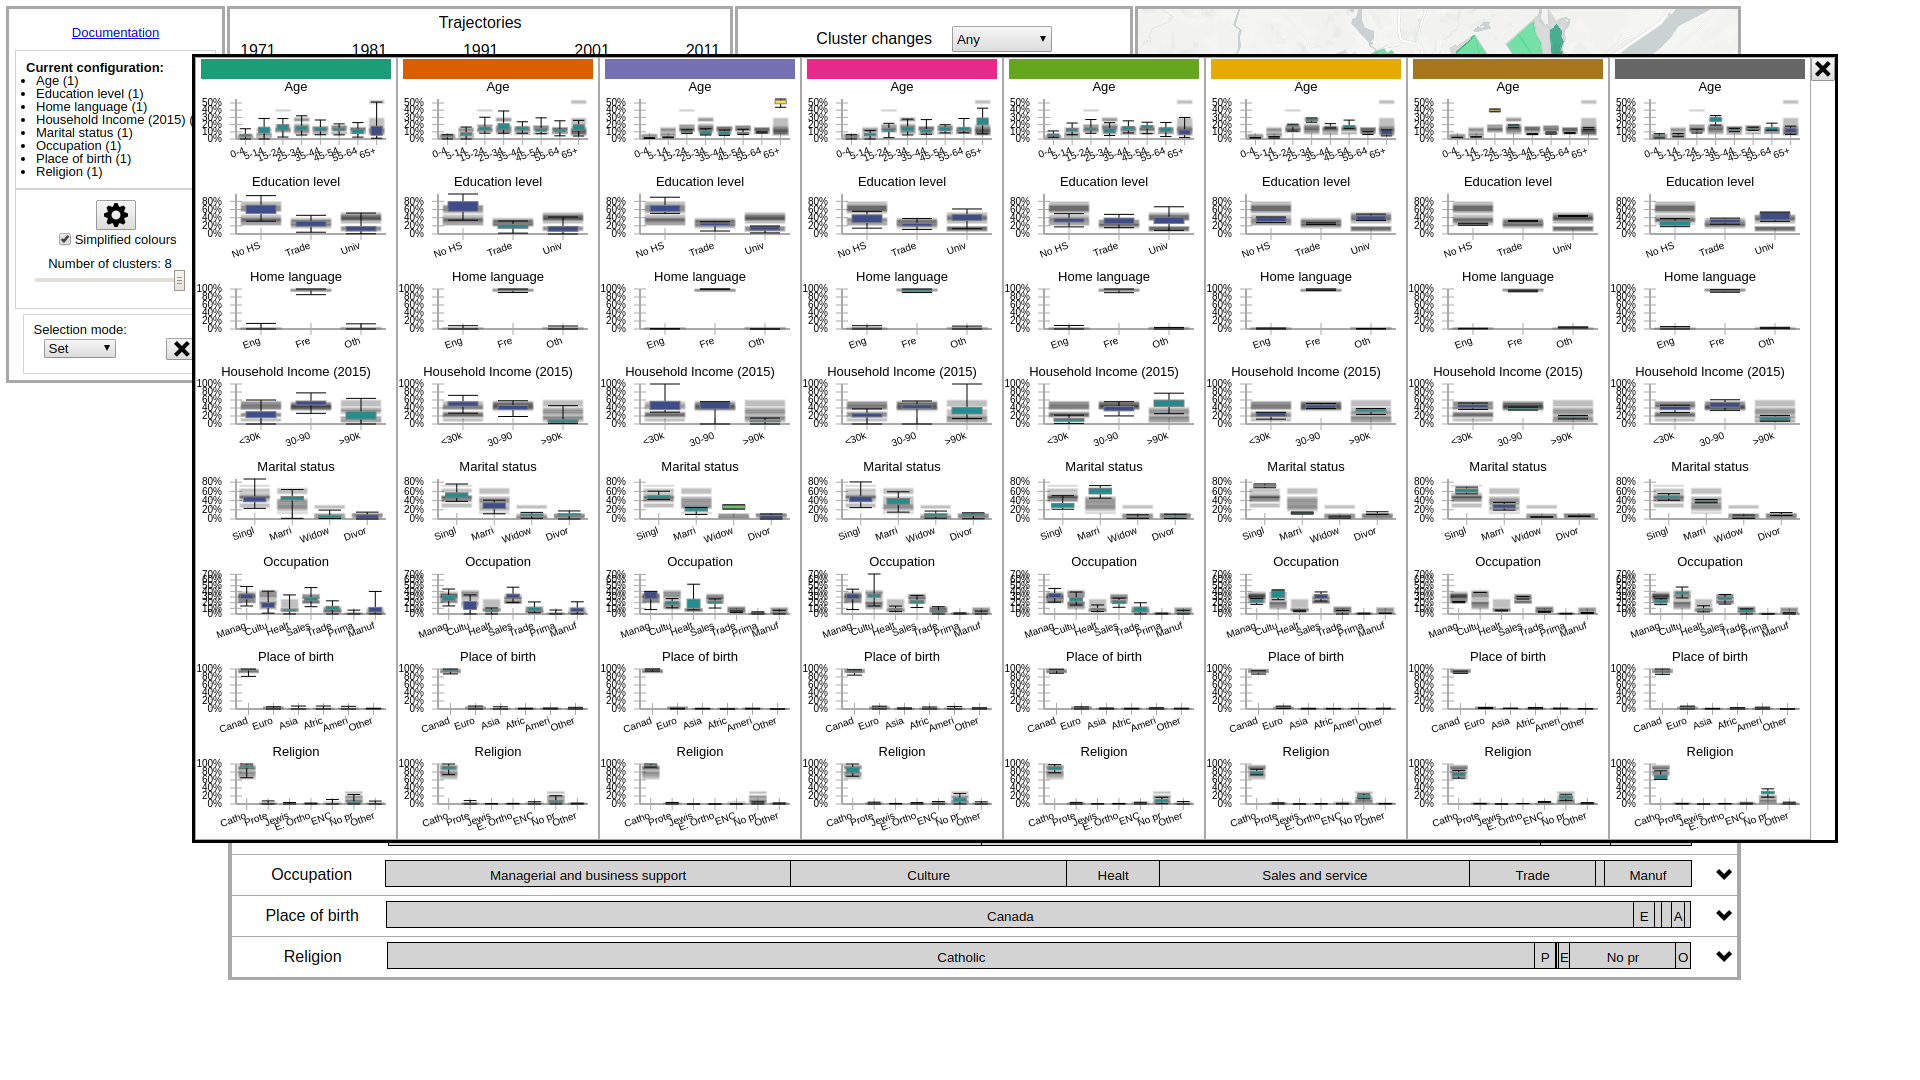
\includegraphics[width=\linewidth]{5b.png}
\end{center}



\subsection{Regina}
\begin{center}
	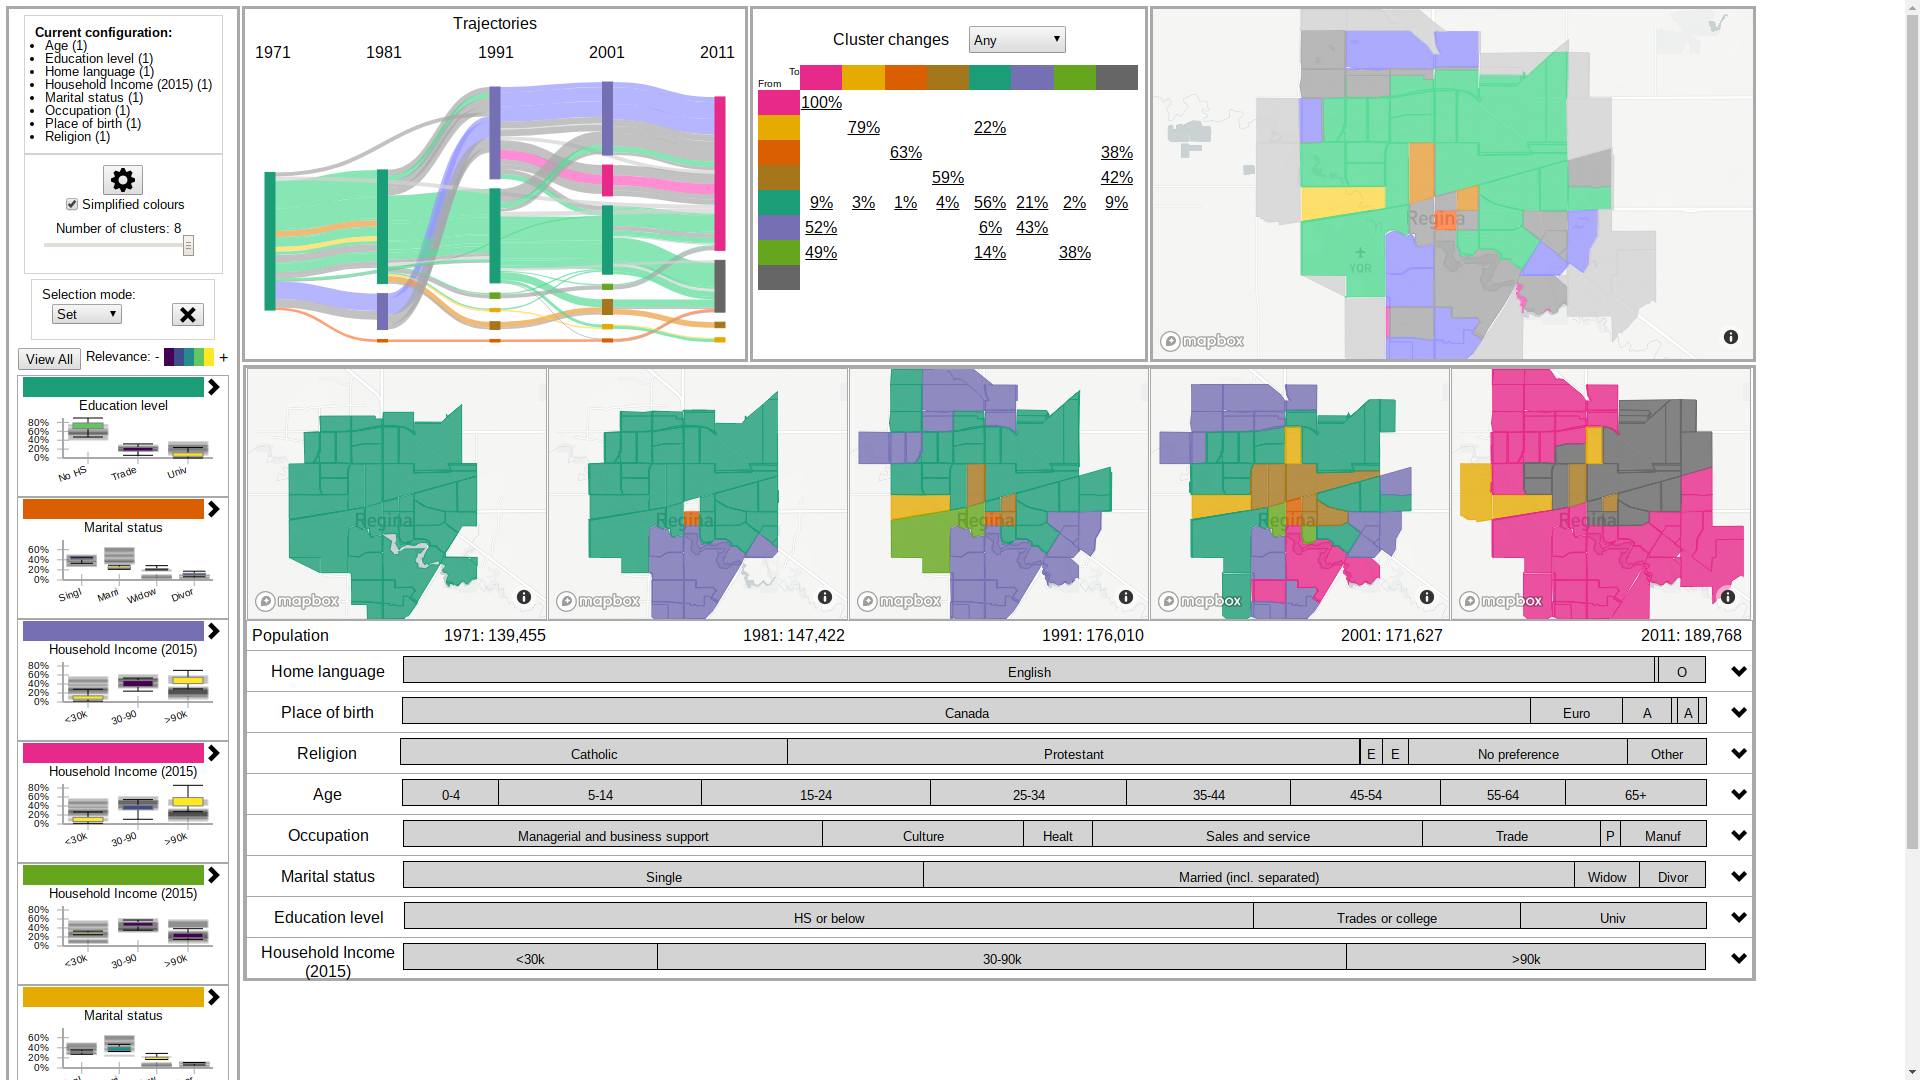
\includegraphics[width=\linewidth]{6a.png}
	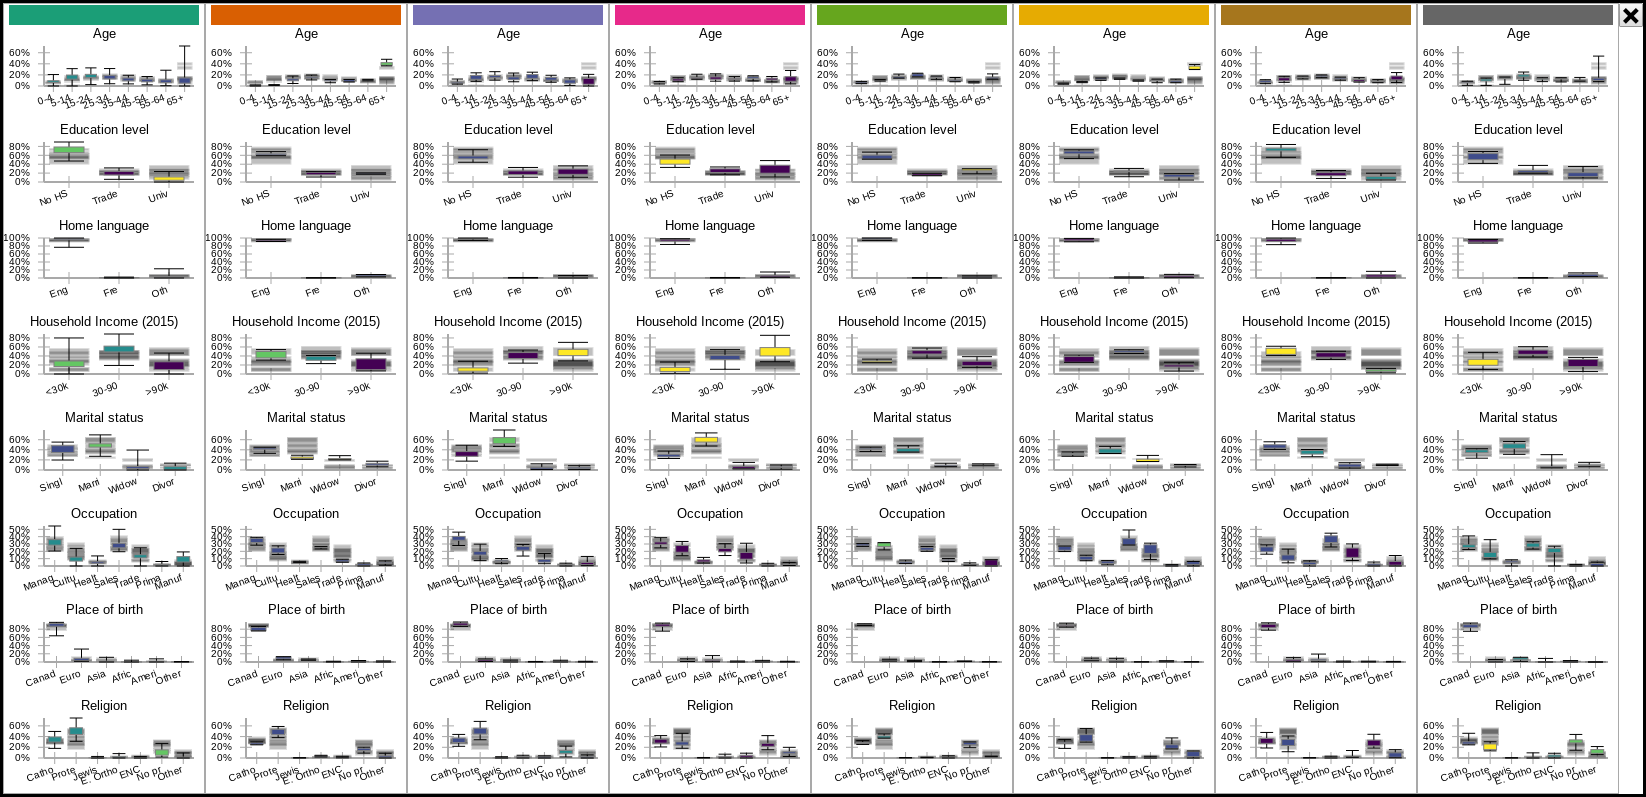
\includegraphics[width=\linewidth]{6b.png}
\end{center}



\subsection{Saskatoon}
\begin{center}
	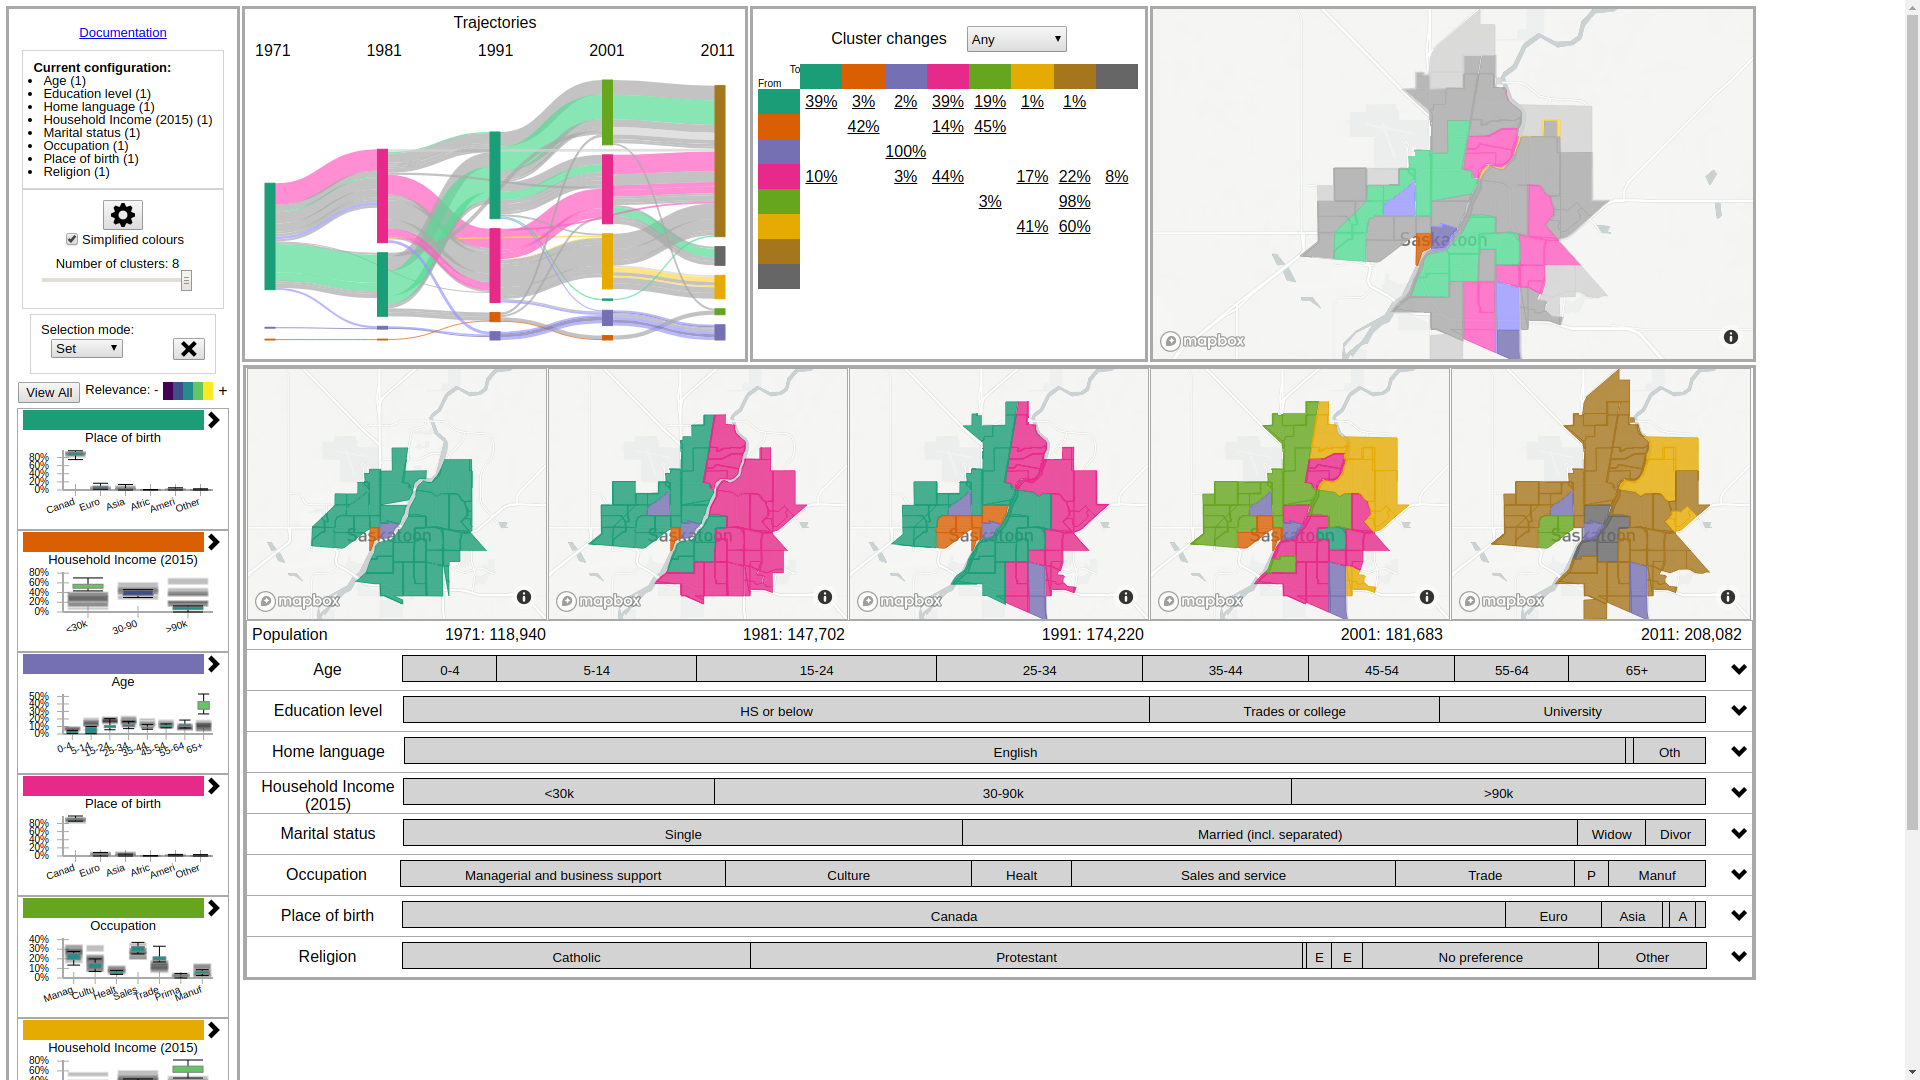
\includegraphics[width=\linewidth]{7a.png}
	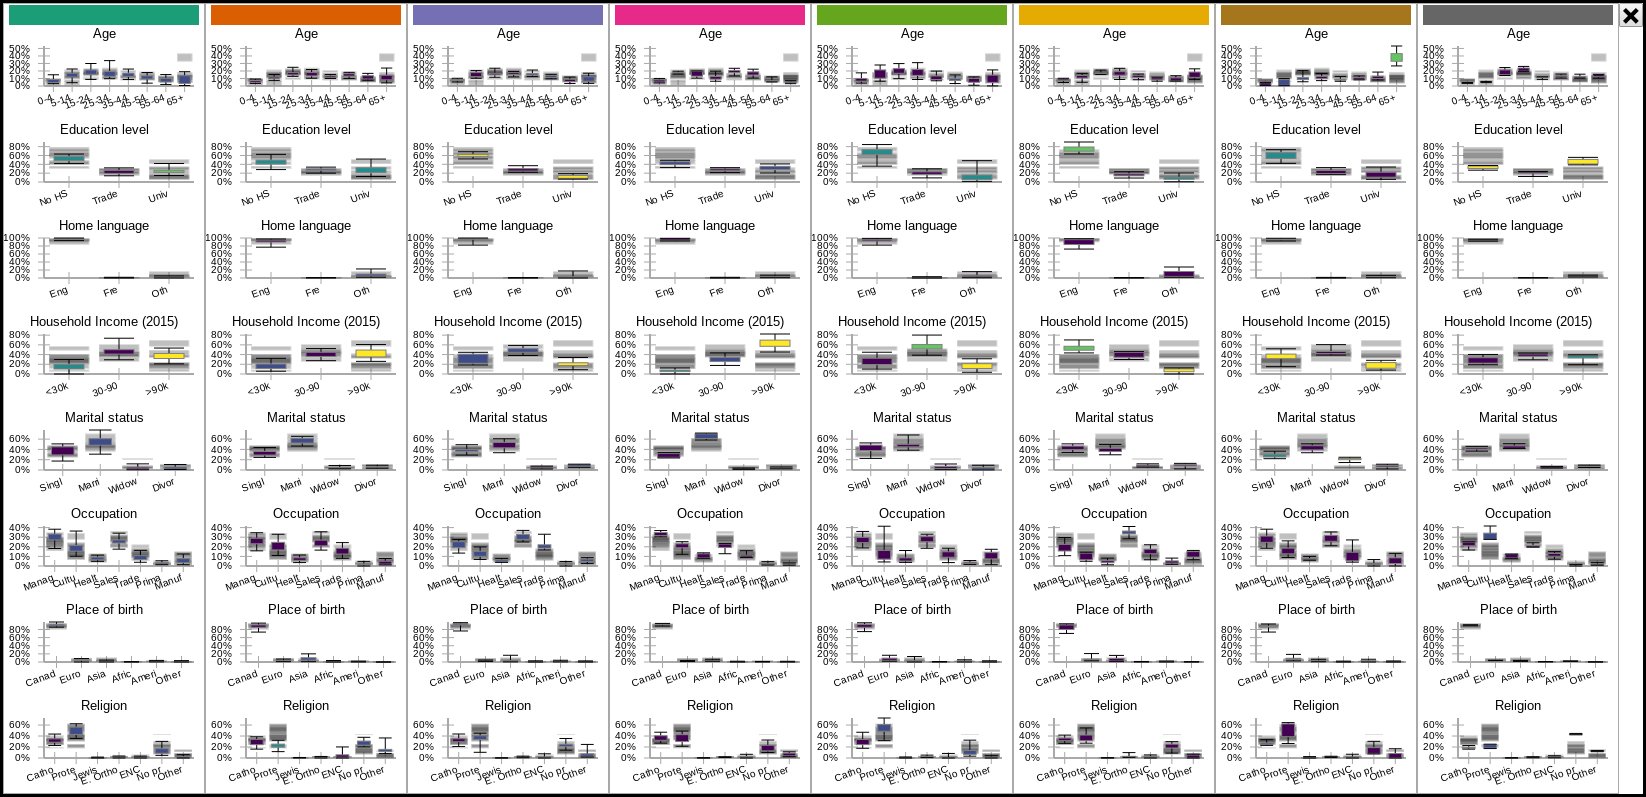
\includegraphics[width=\linewidth]{7b.png}
\end{center}



\subsection{St John}
\begin{center}
	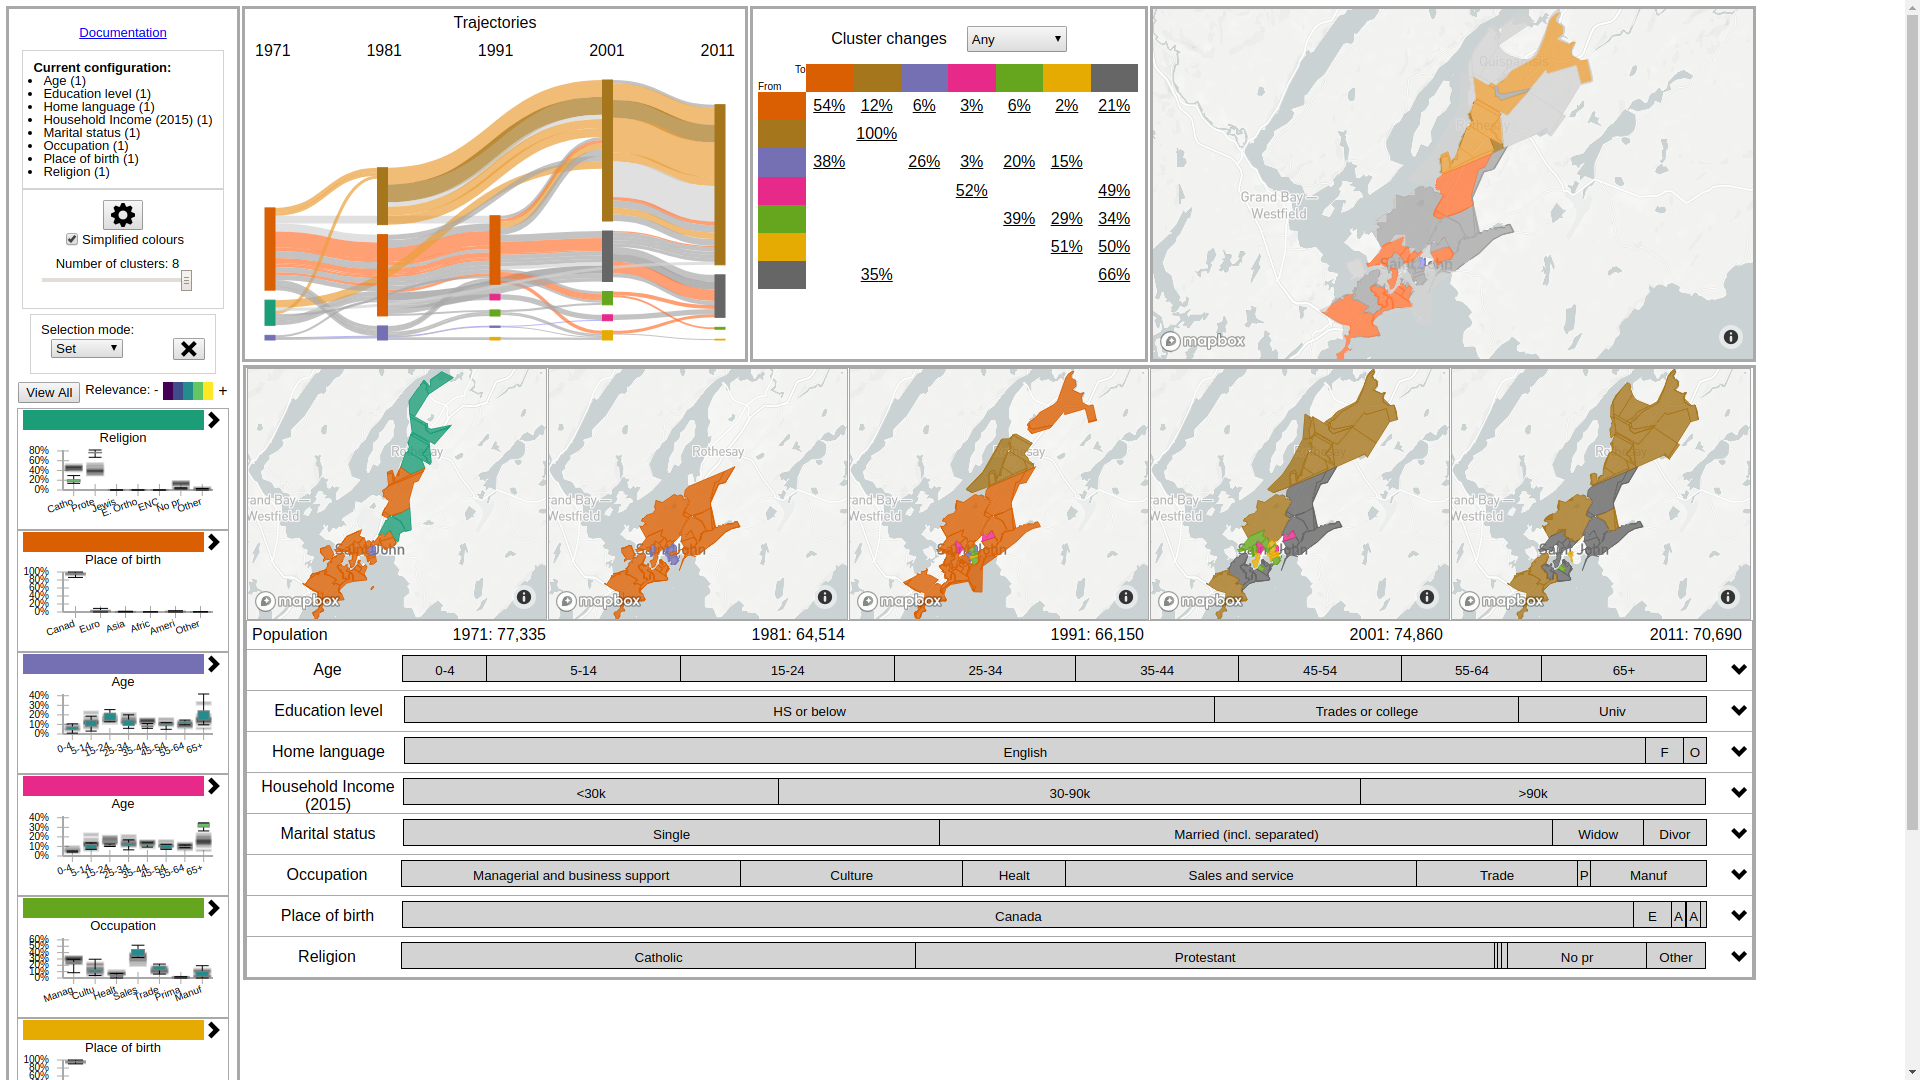
\includegraphics[width=\linewidth]{8a.png}
	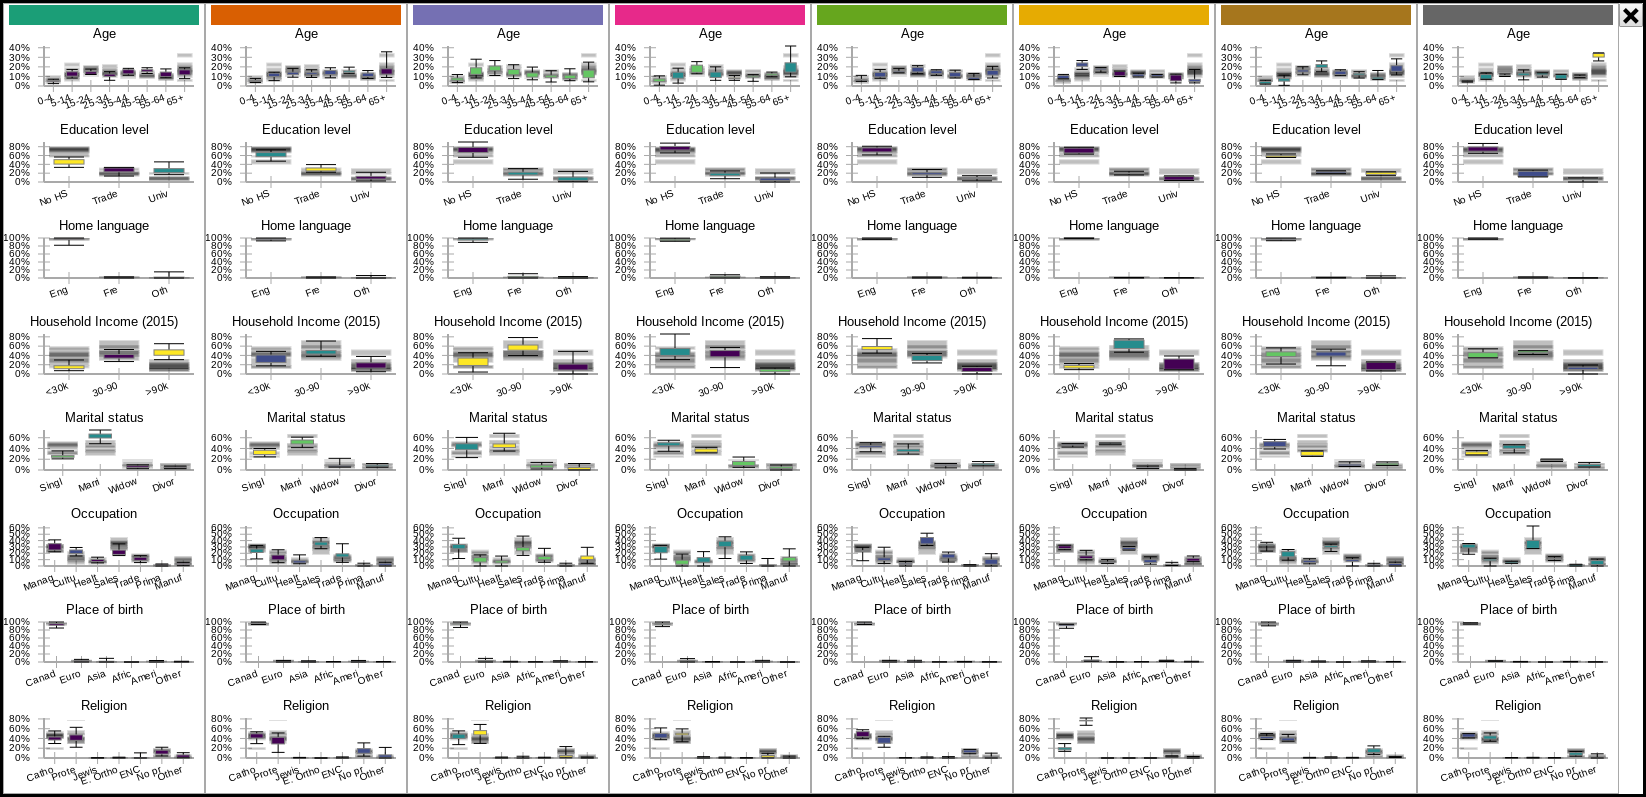
\includegraphics[width=\linewidth]{8b.png}
\end{center}



\subsection{Winnipeg}
\begin{center}
	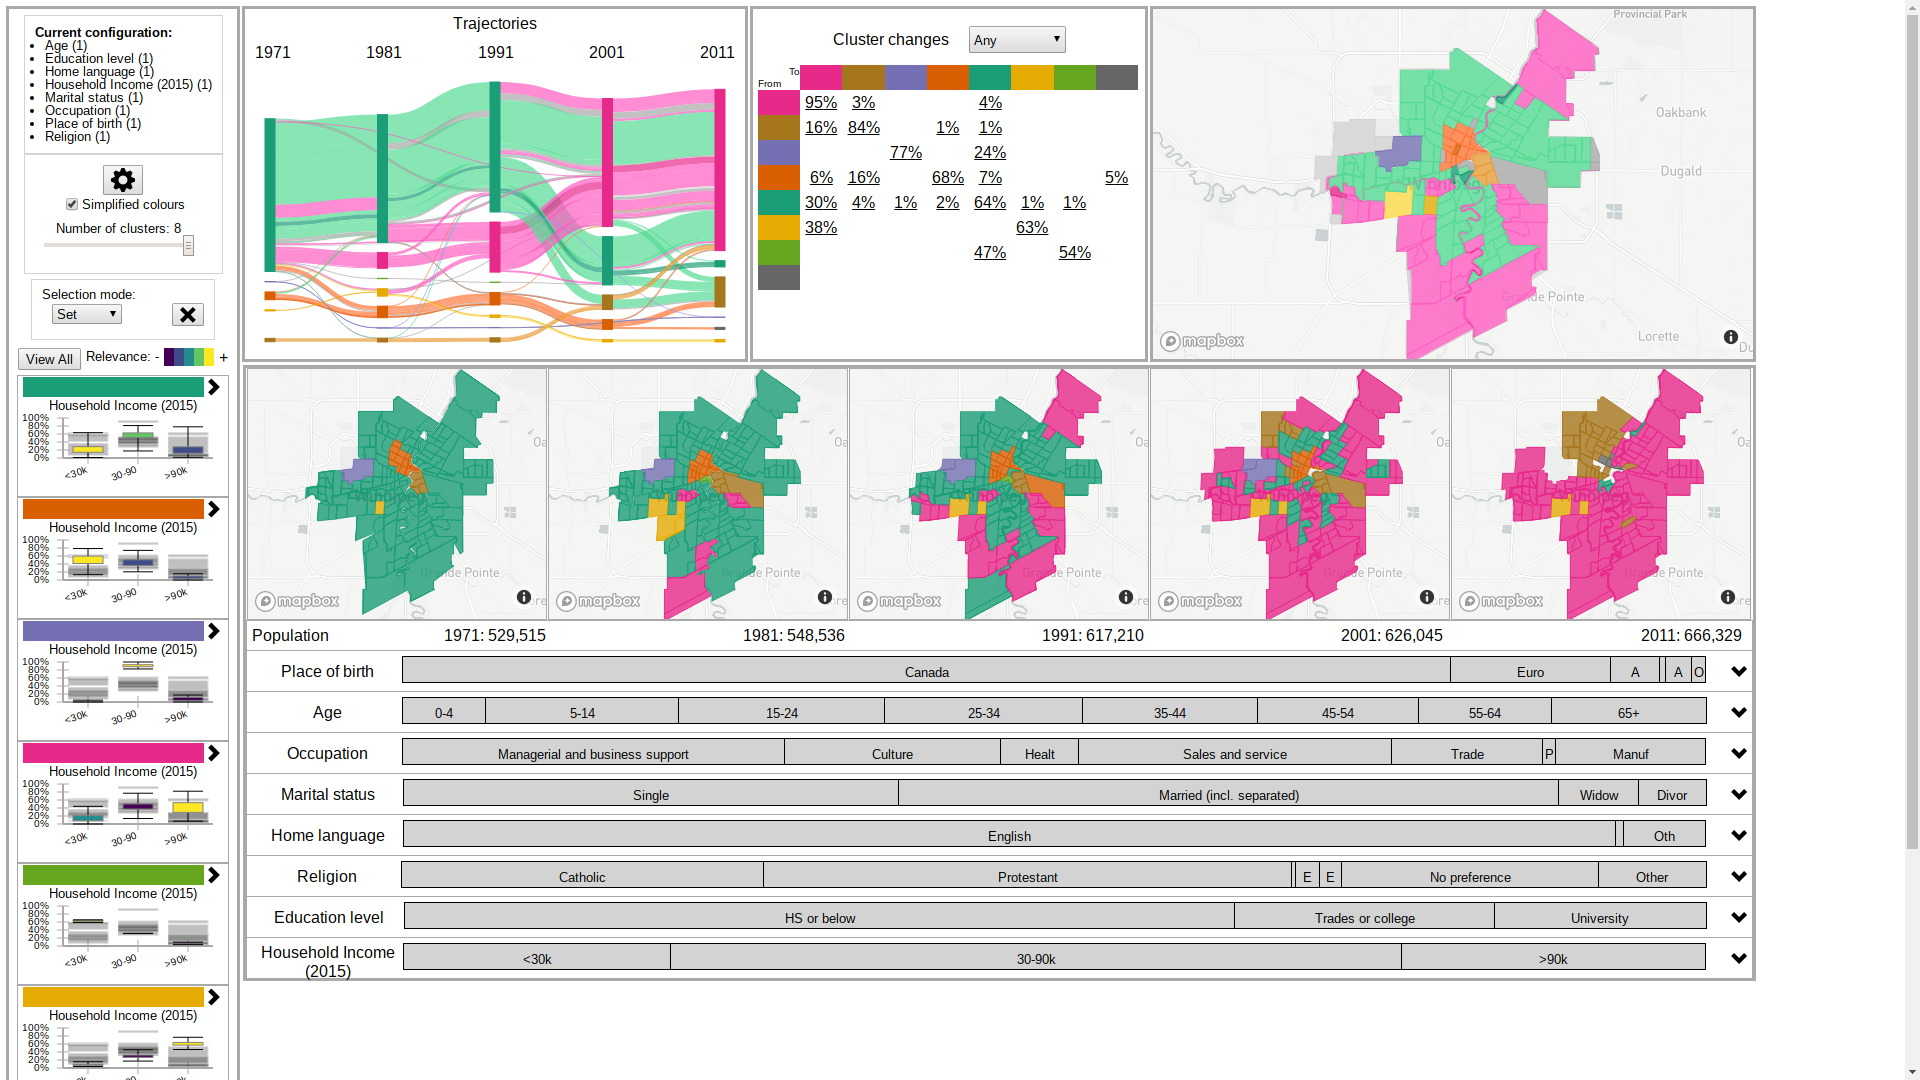
\includegraphics[width=\linewidth]{9a.png}
	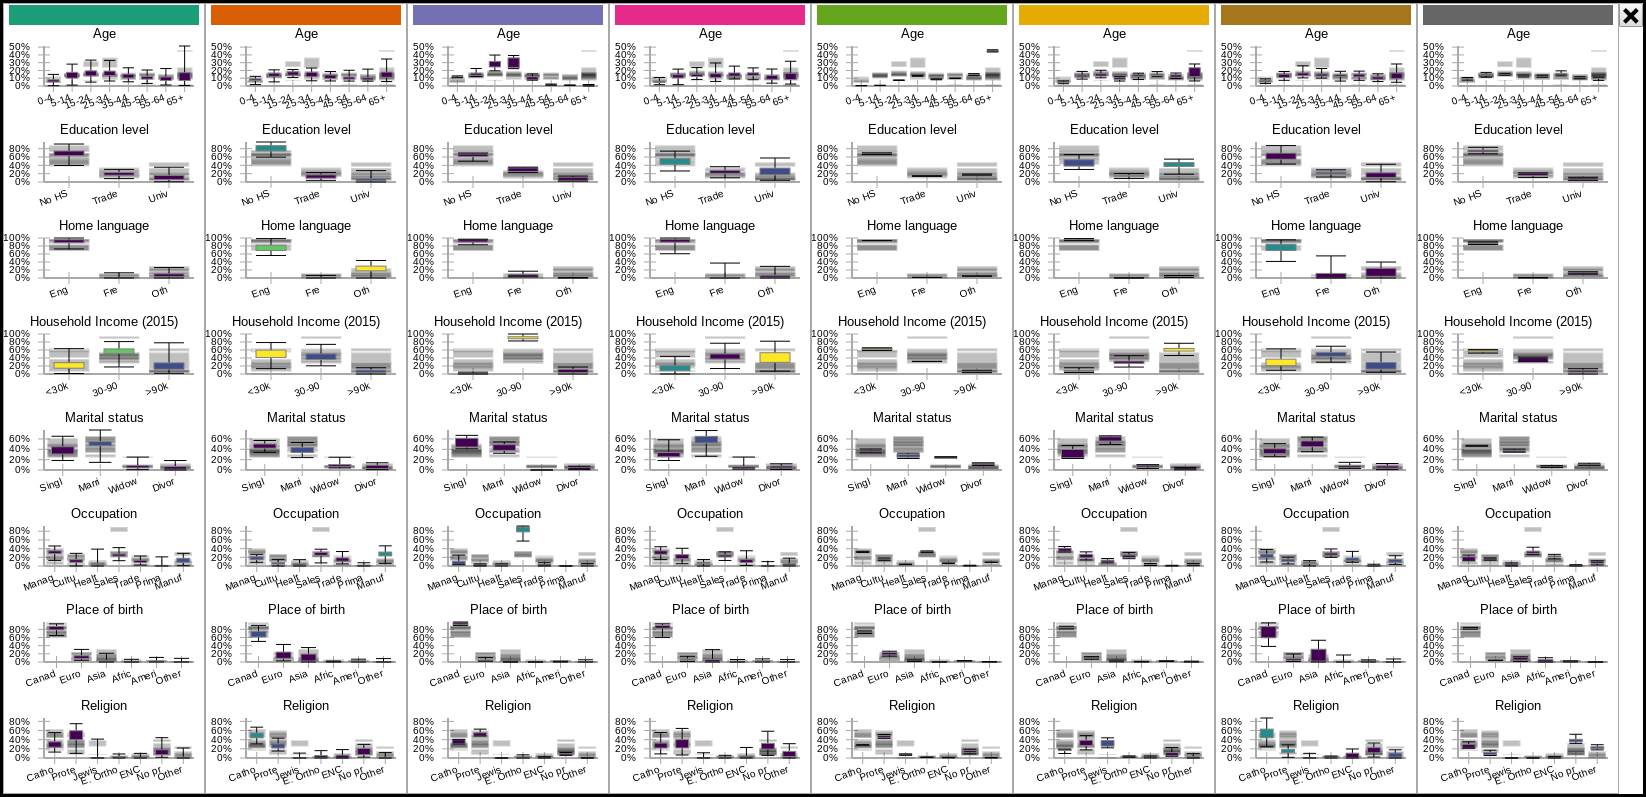
\includegraphics[width=\linewidth]{9b.png}
\end{center}



\subsection{LA County}
\begin{center}
	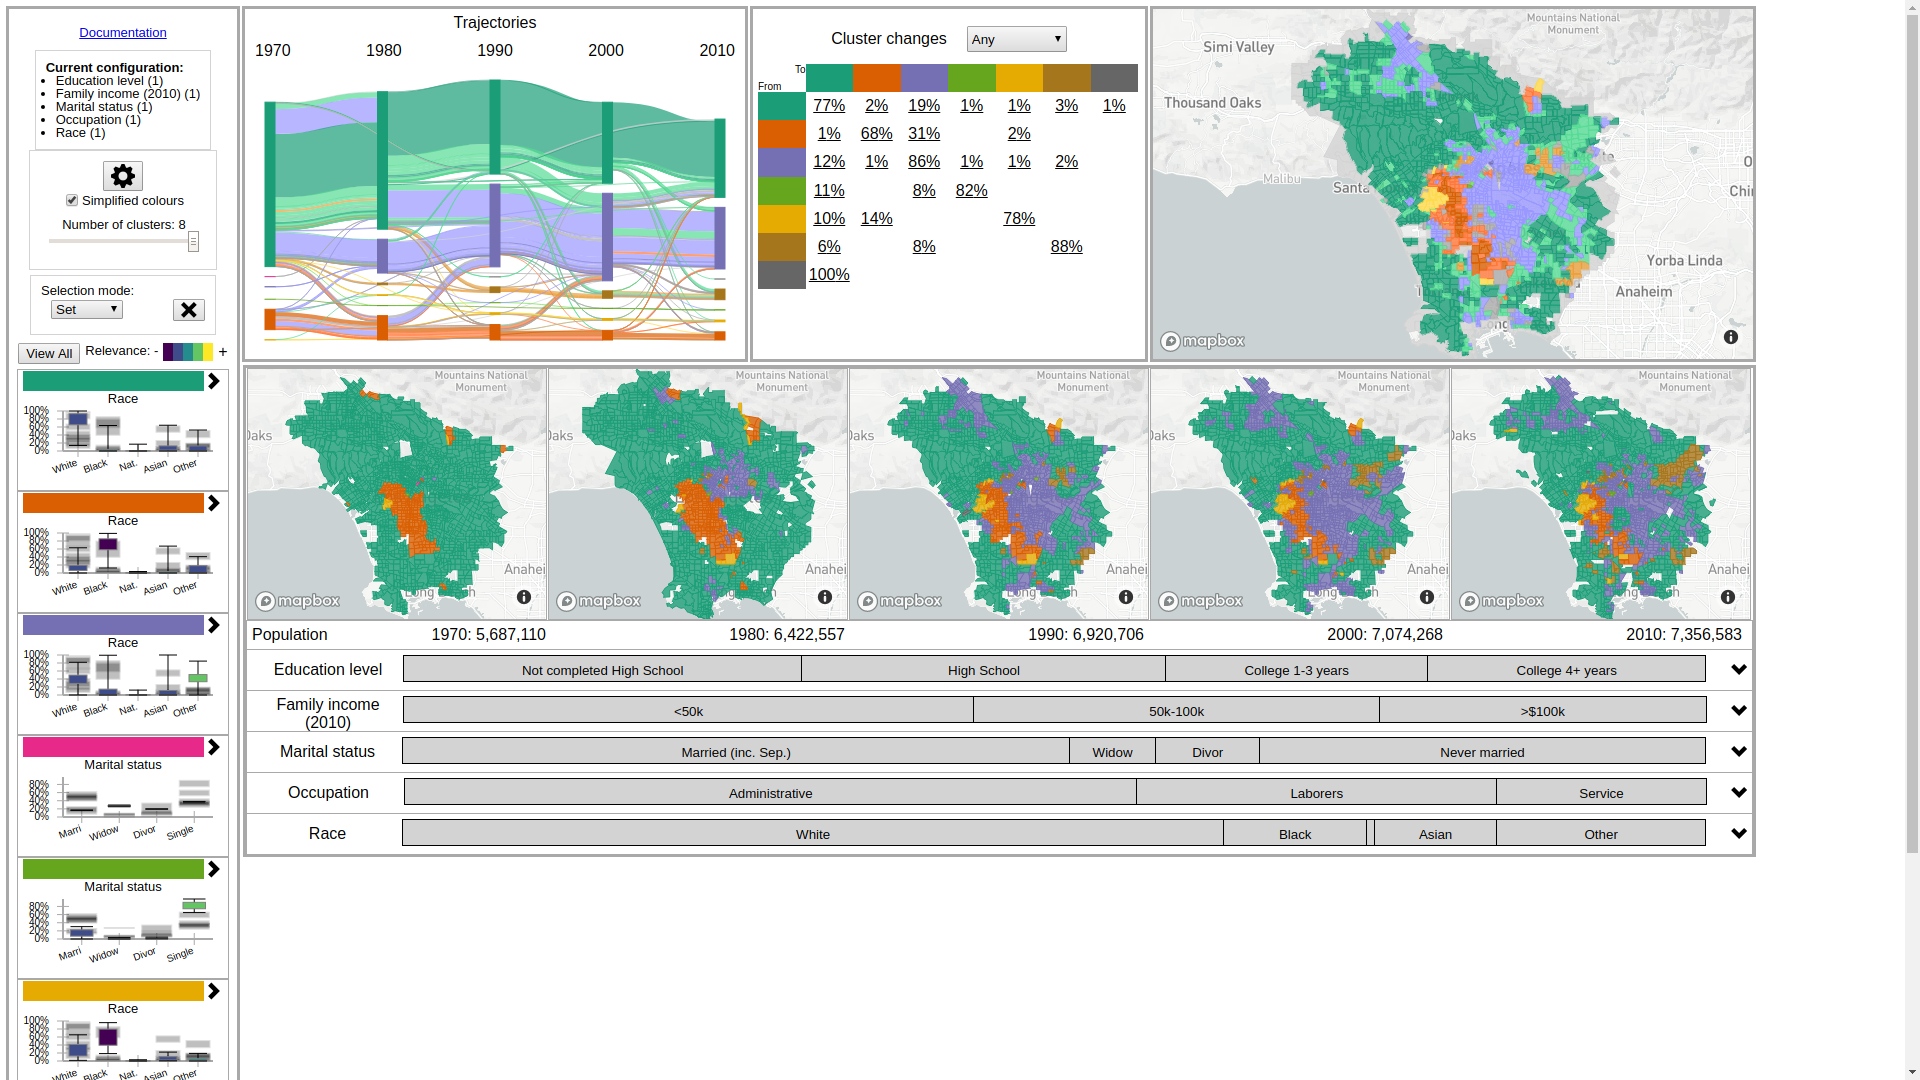
\includegraphics[width=\linewidth]{10a.png}
	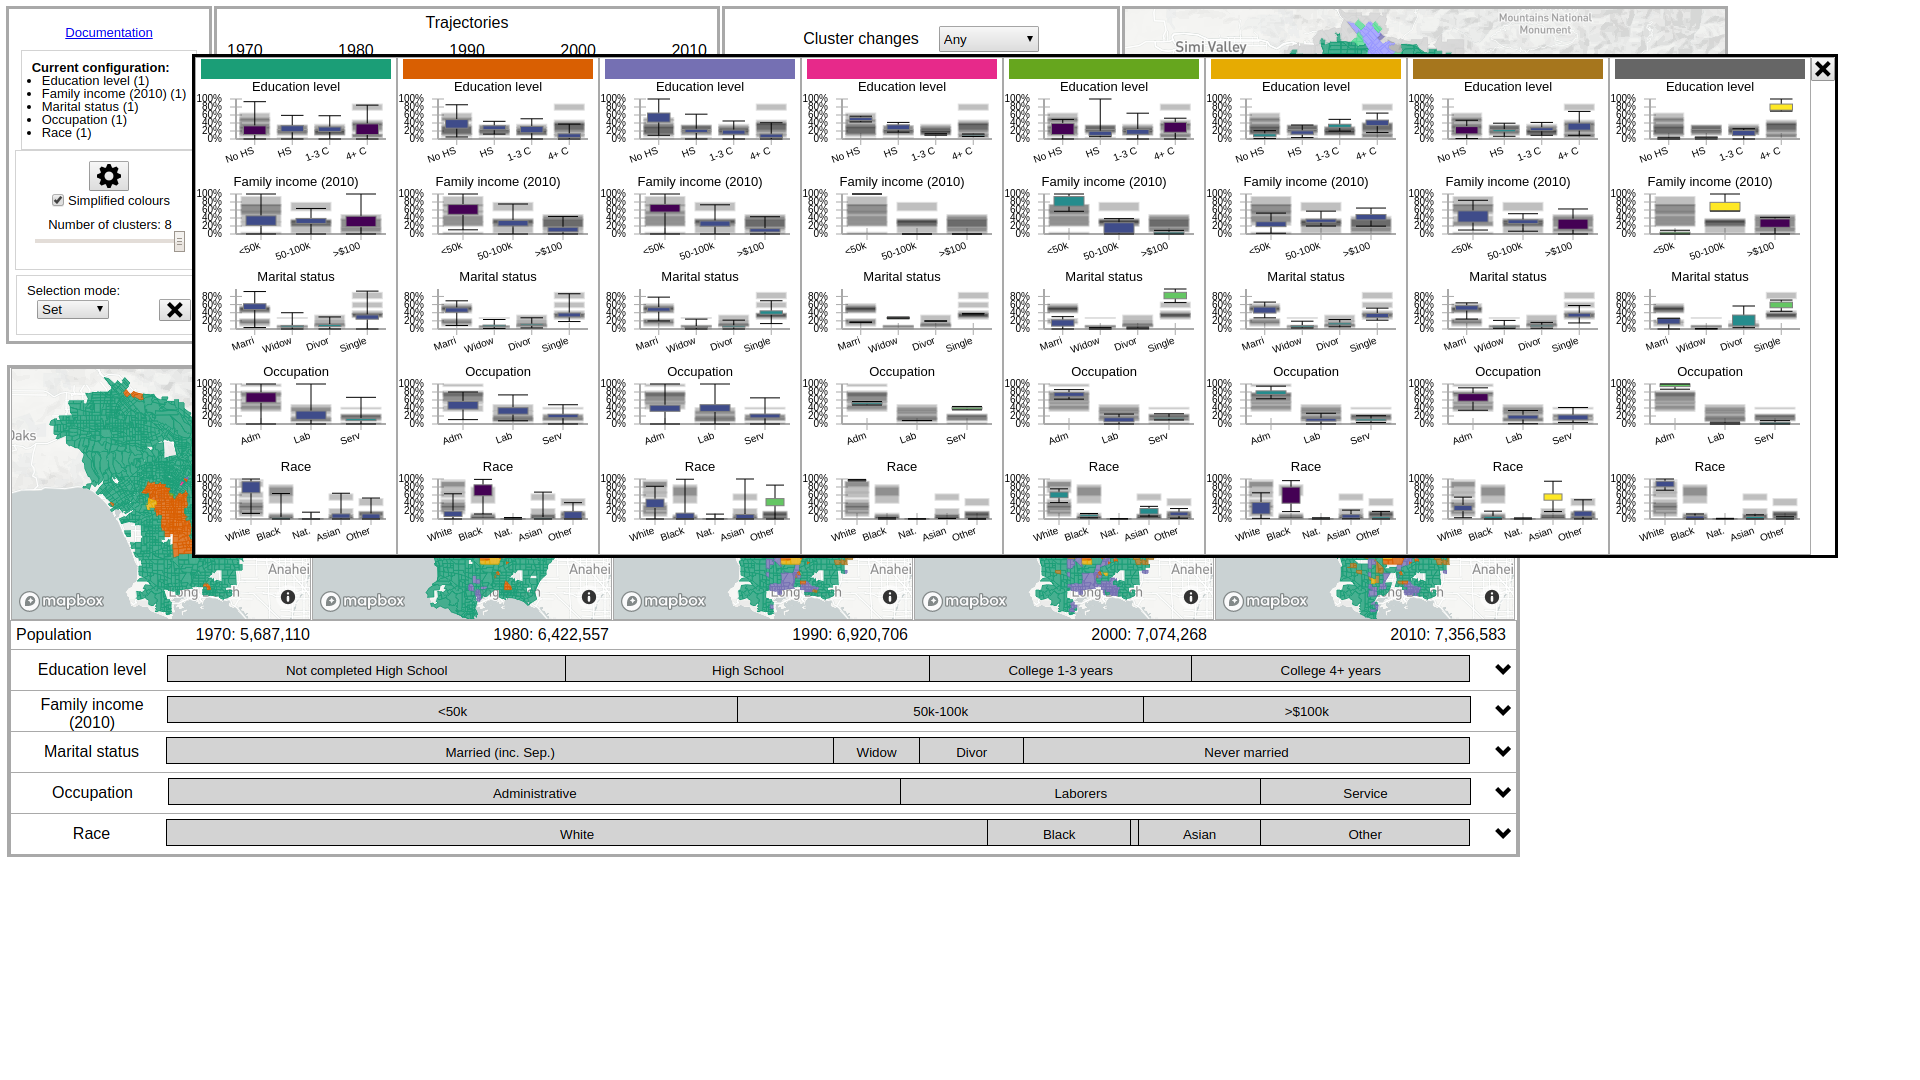
\includegraphics[width=\linewidth]{10b.png}
\end{center}
\clearpage


\subsection{Staten Island}
\begin{center}
	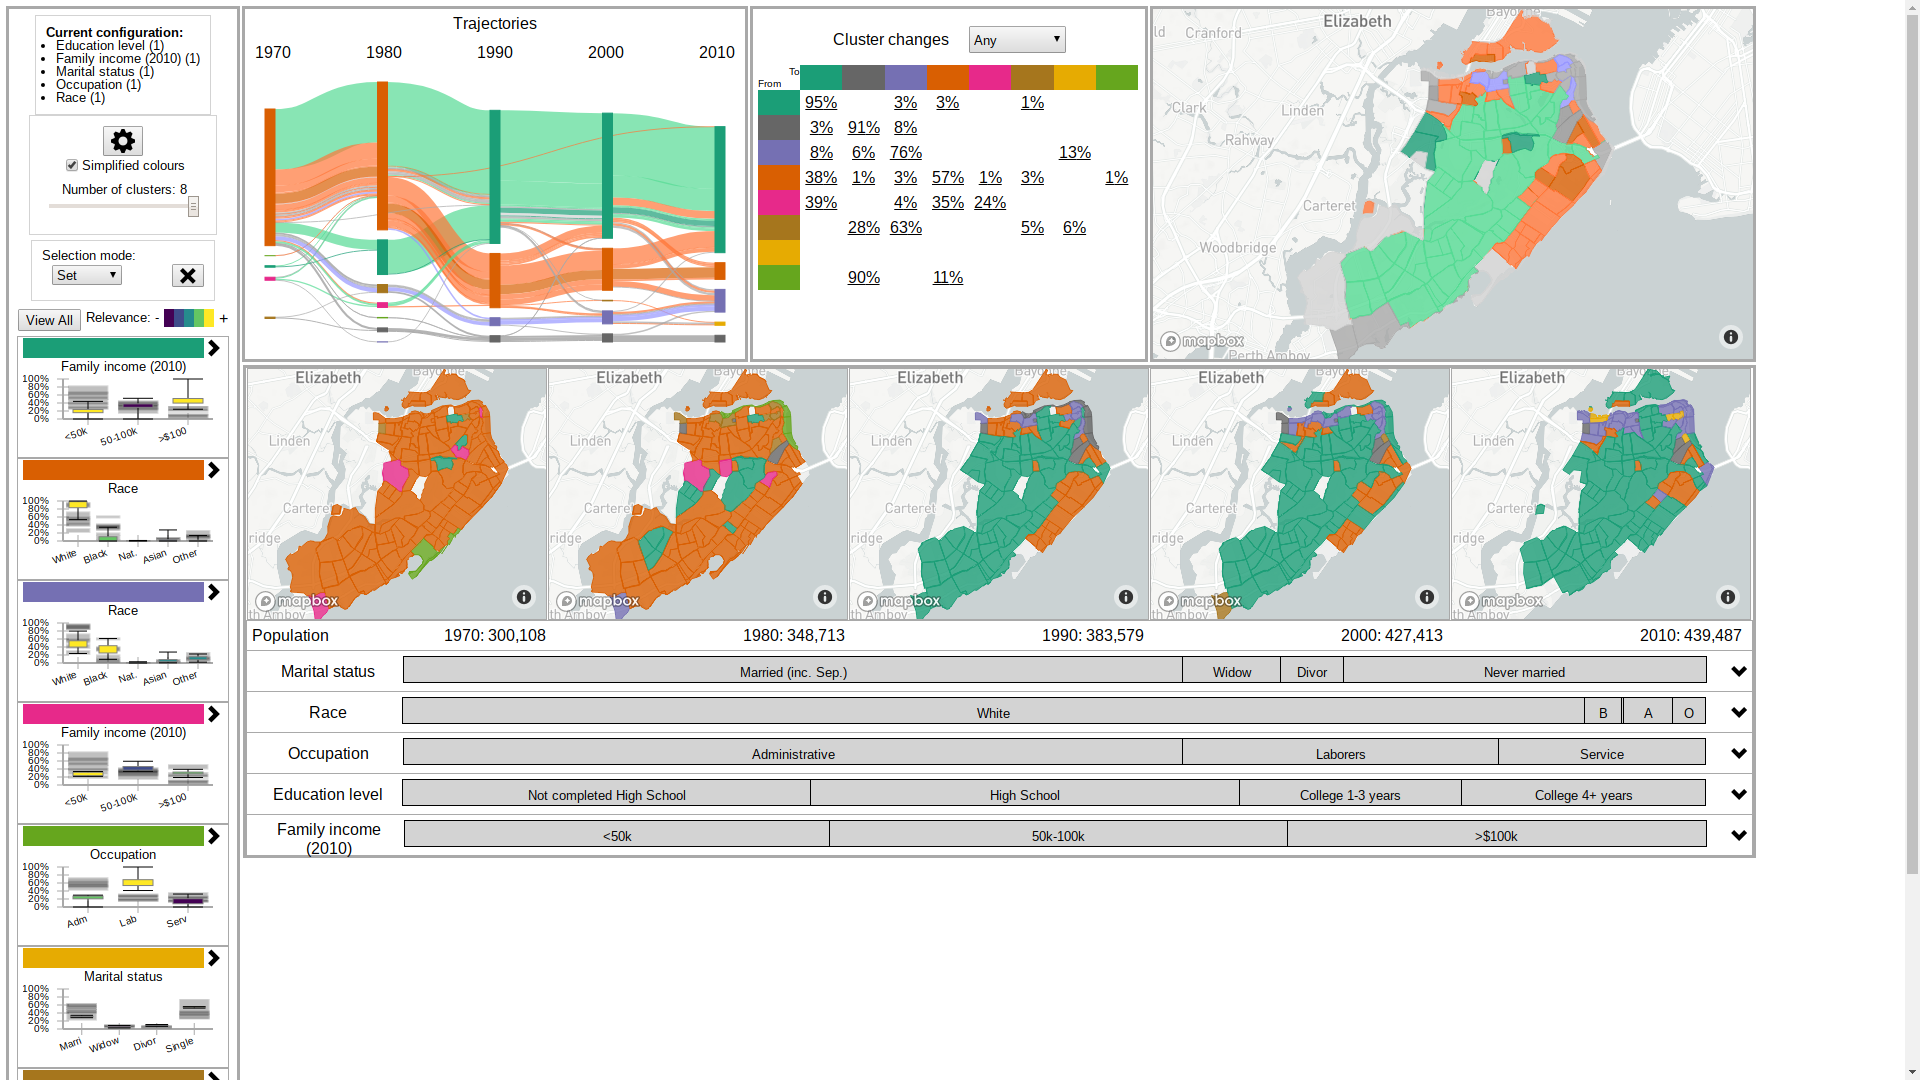
\includegraphics[width=\linewidth]{11a.png}
	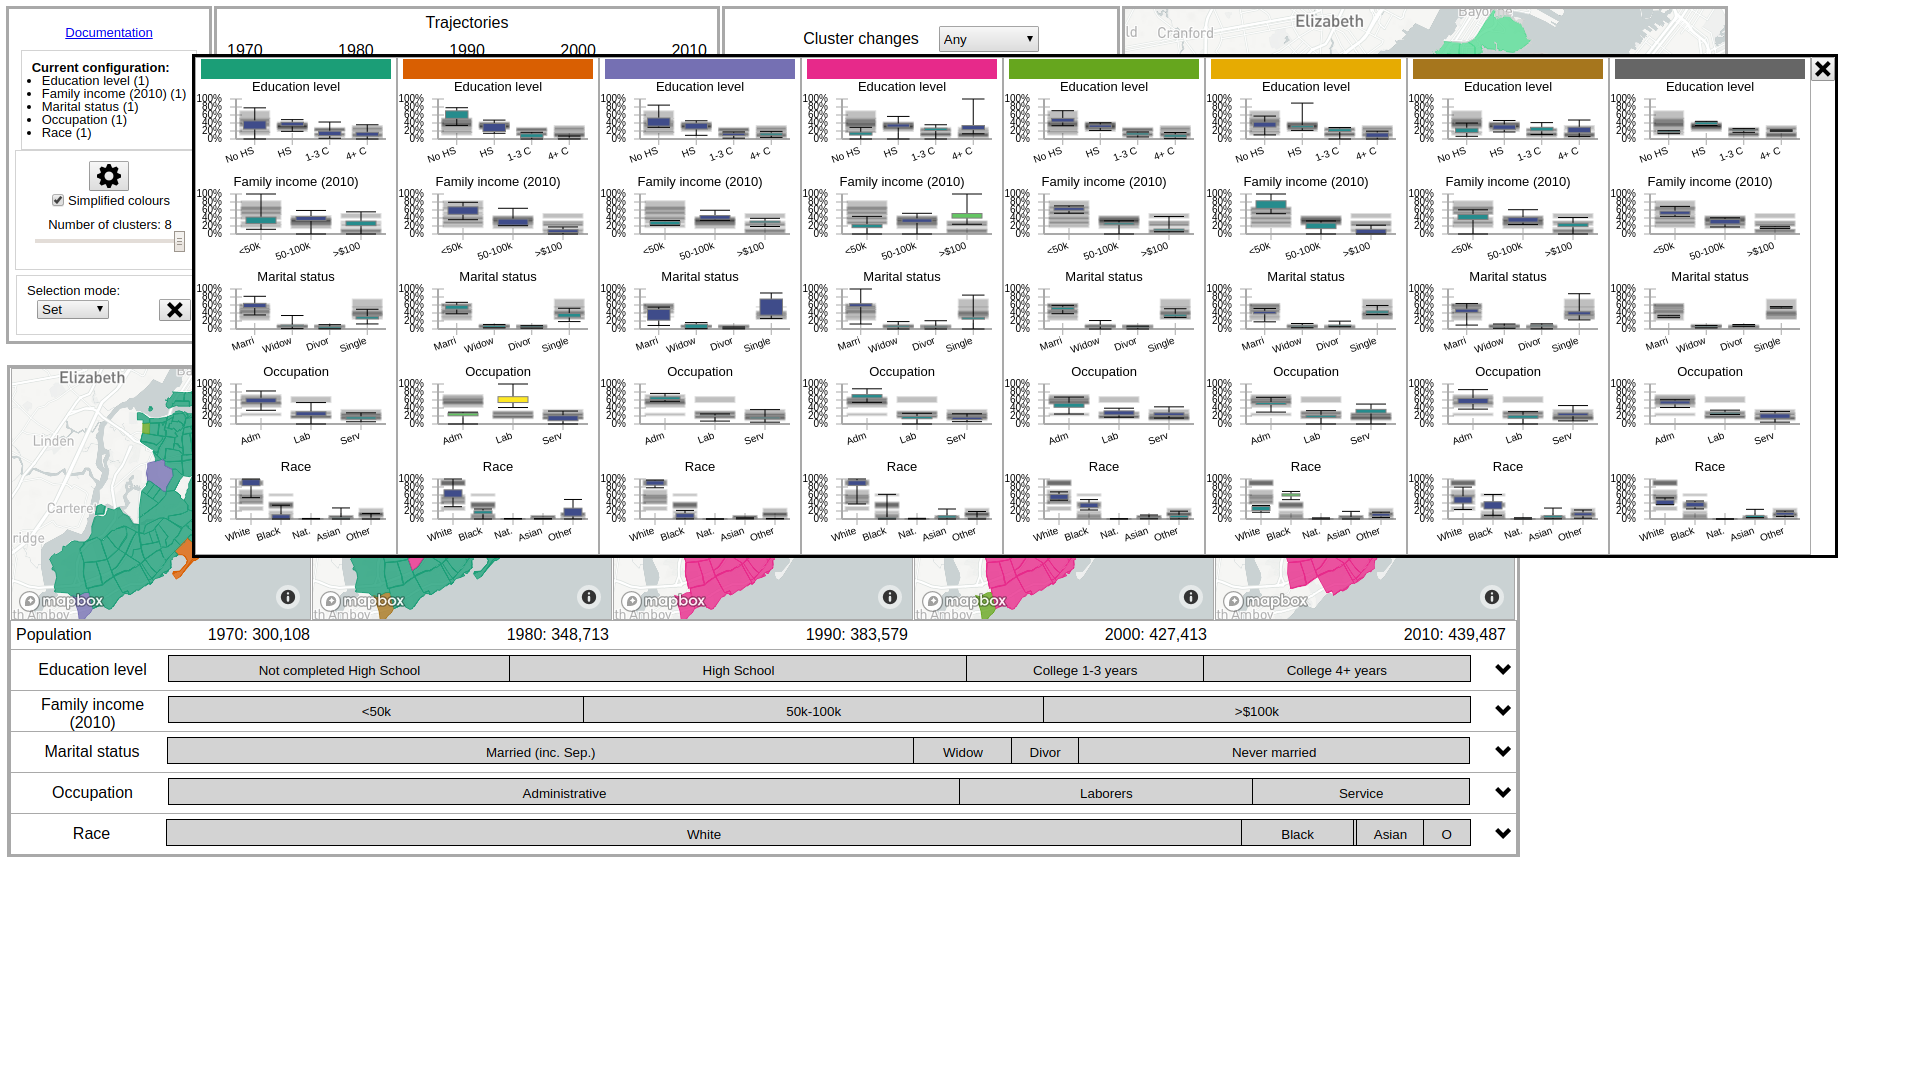
\includegraphics[width=\linewidth]{11b.png}
\end{center} \clearpage



\subsection{Manhattan}
\begin{center}
	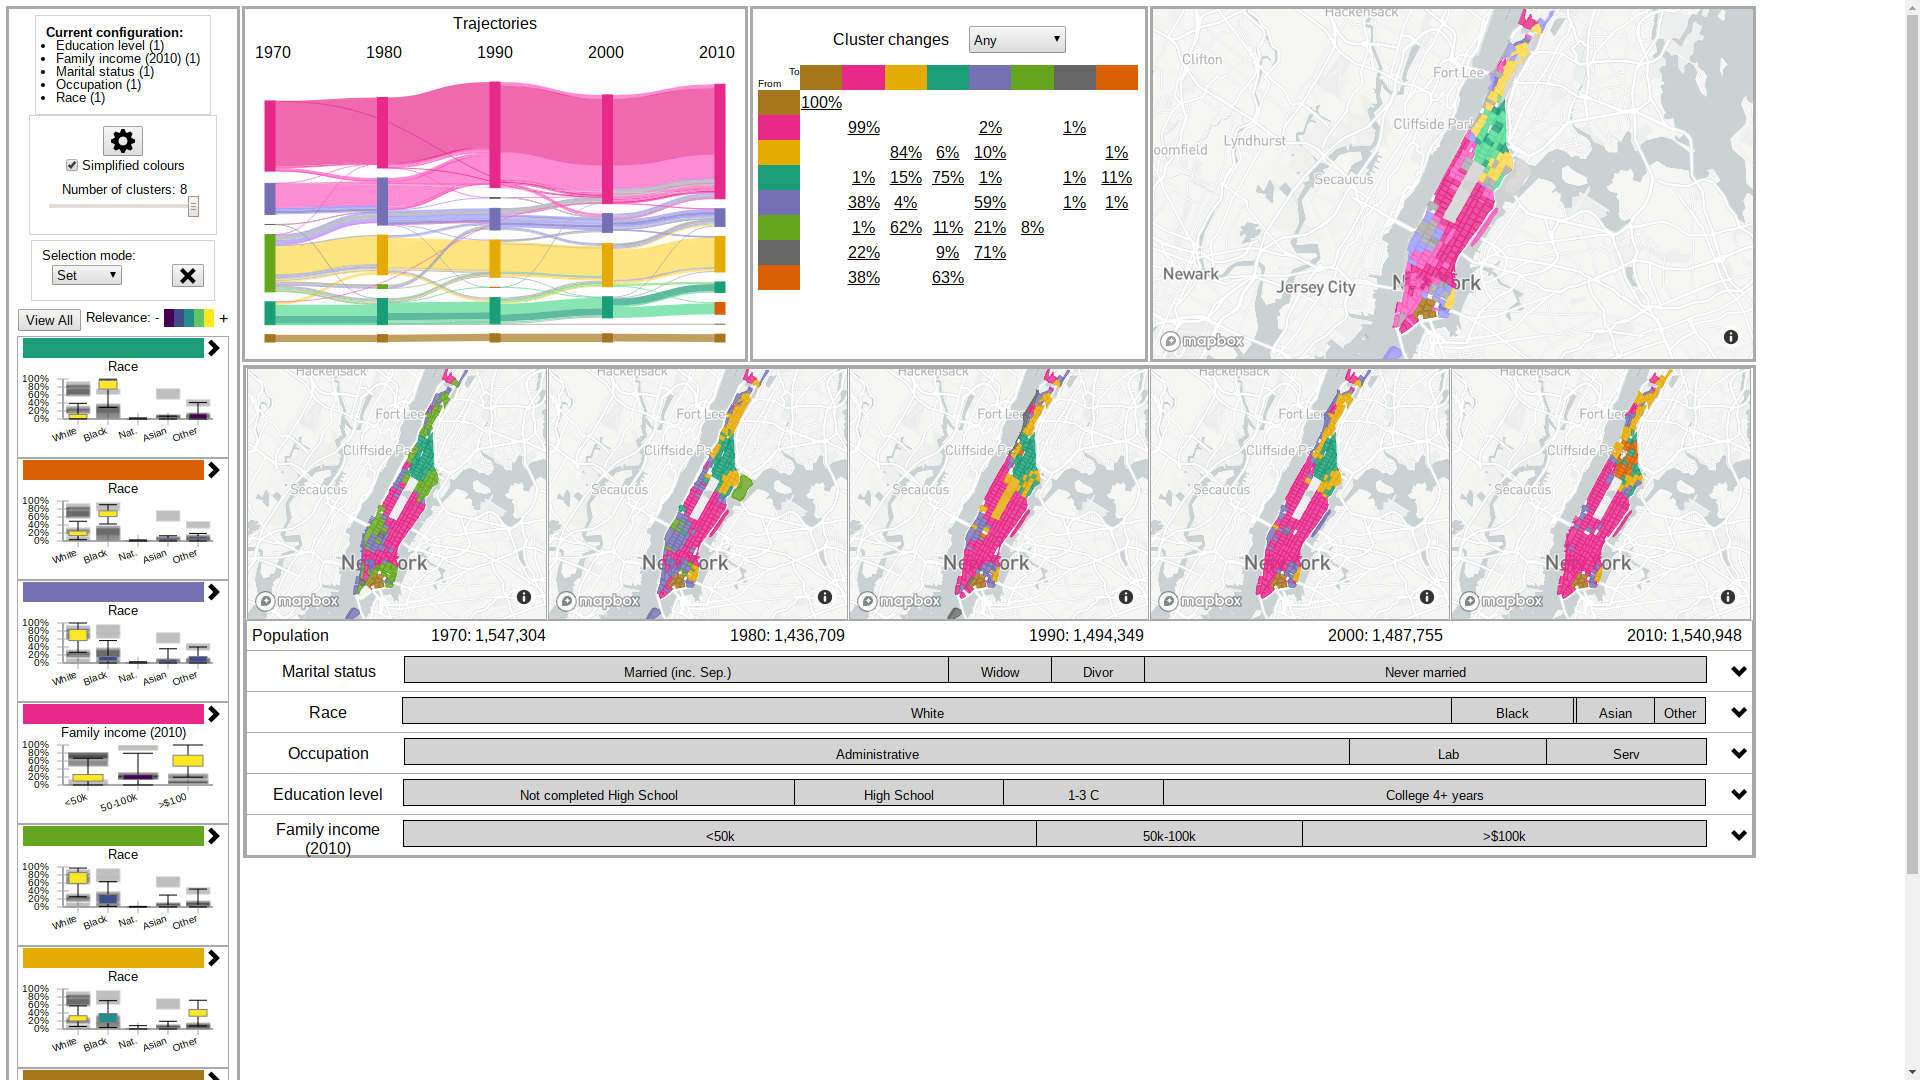
\includegraphics[width=\linewidth]{12a.png}
	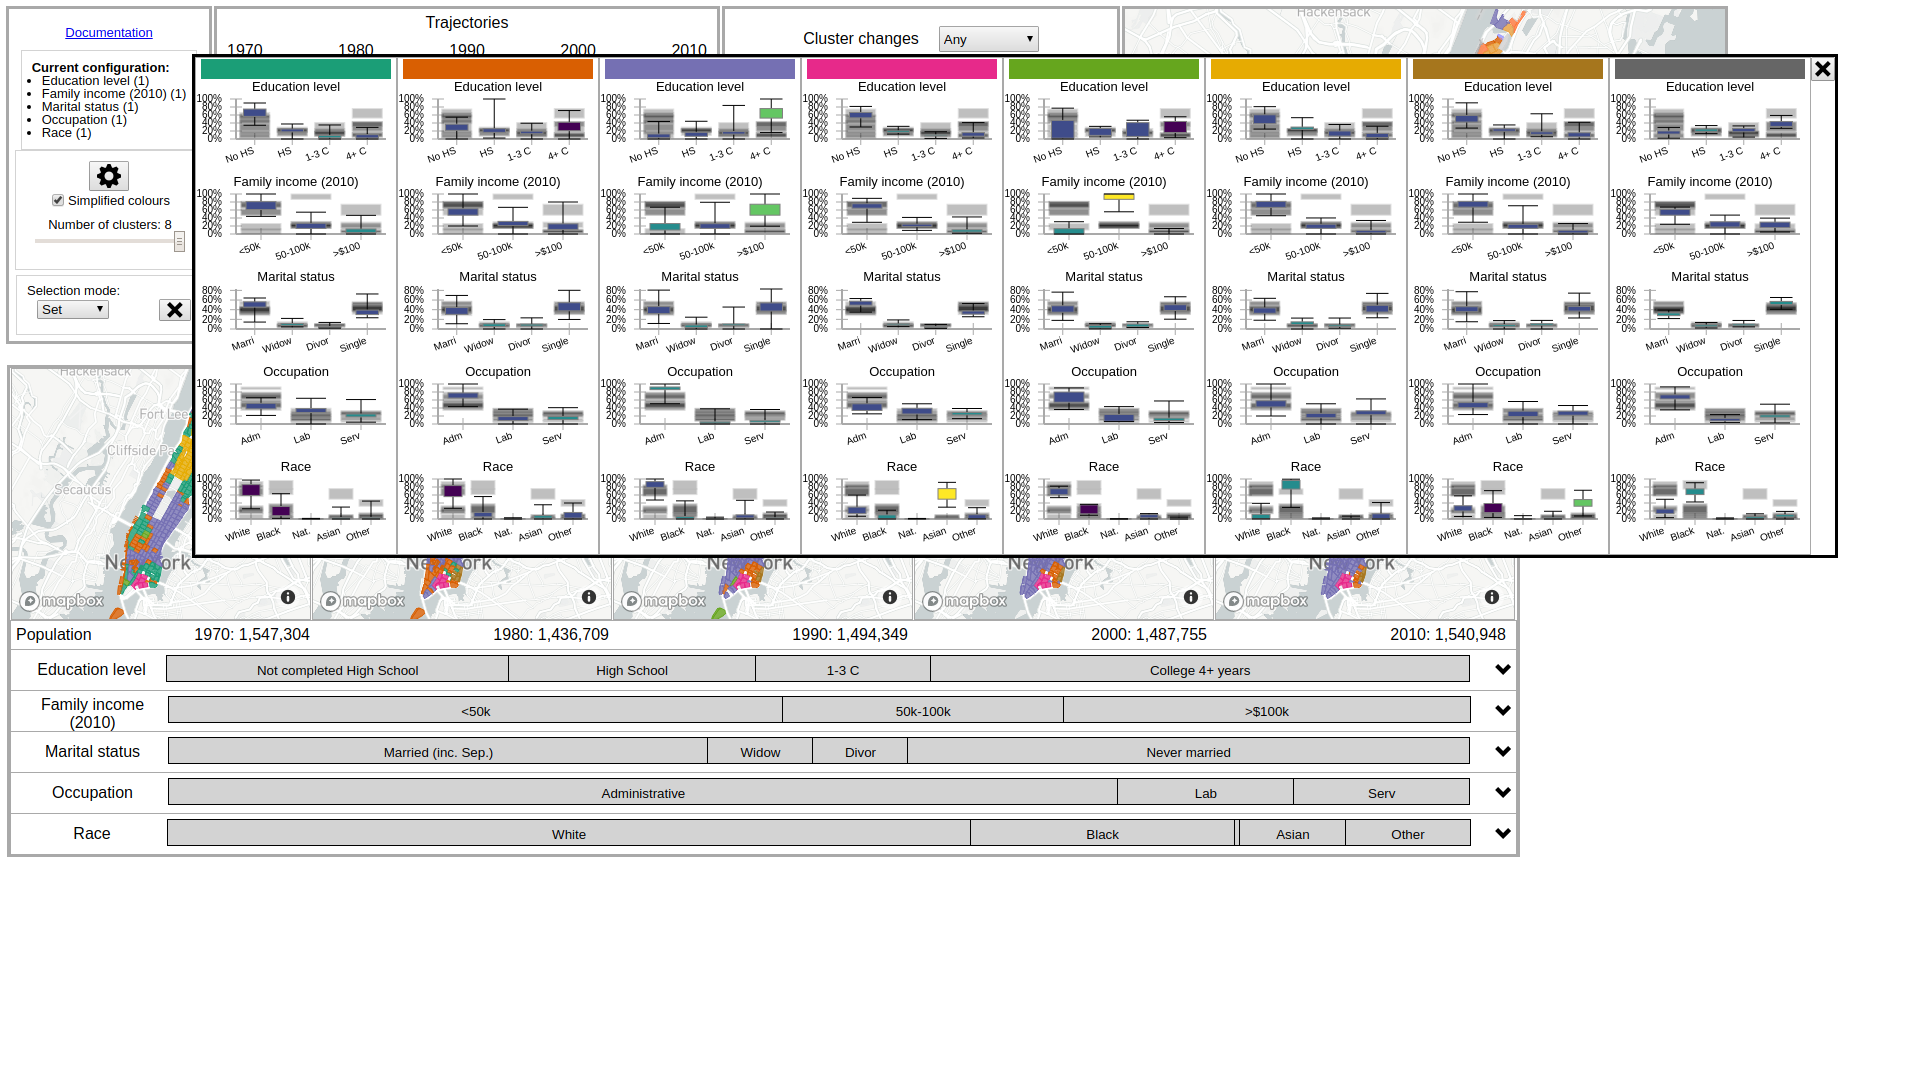
\includegraphics[width=\linewidth]{12b.png}
\end{center} \clearpage



\subsection{Queens}
\begin{center}
	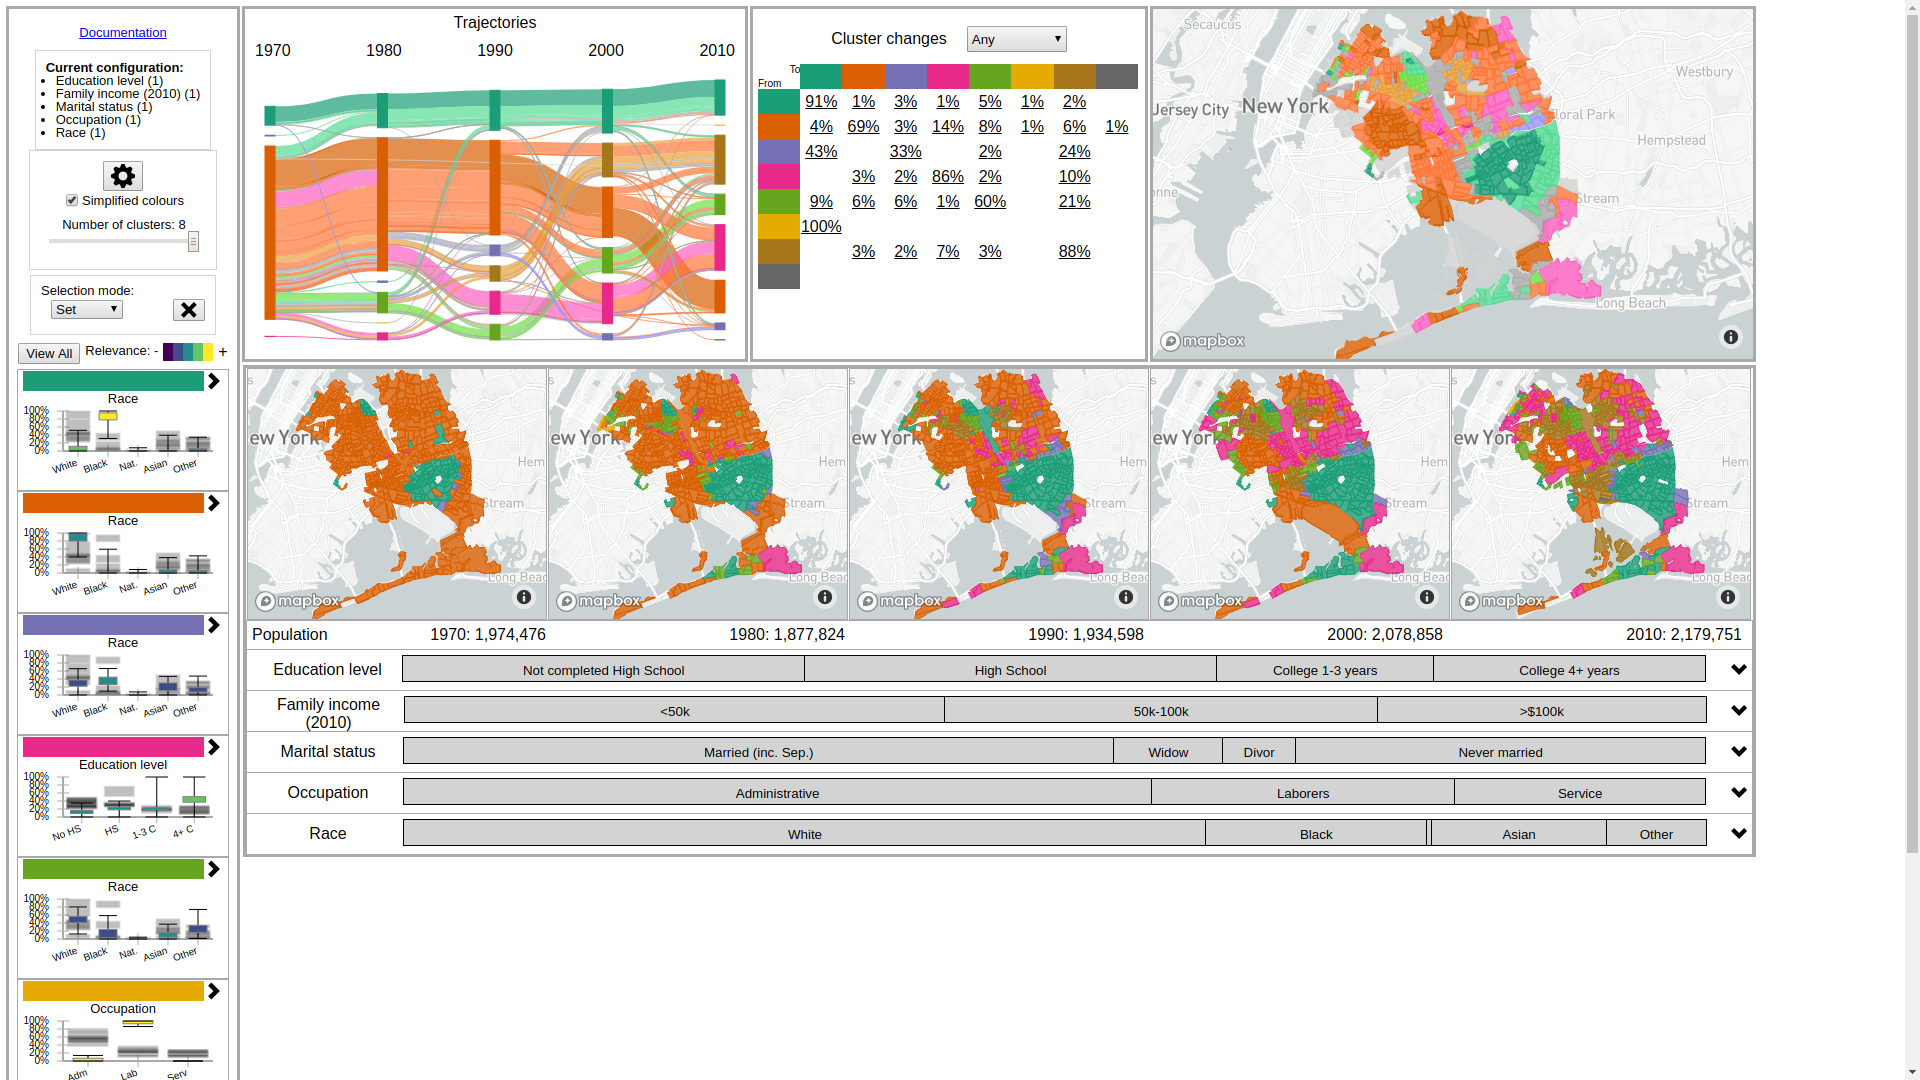
\includegraphics[width=\linewidth]{13a.png}
	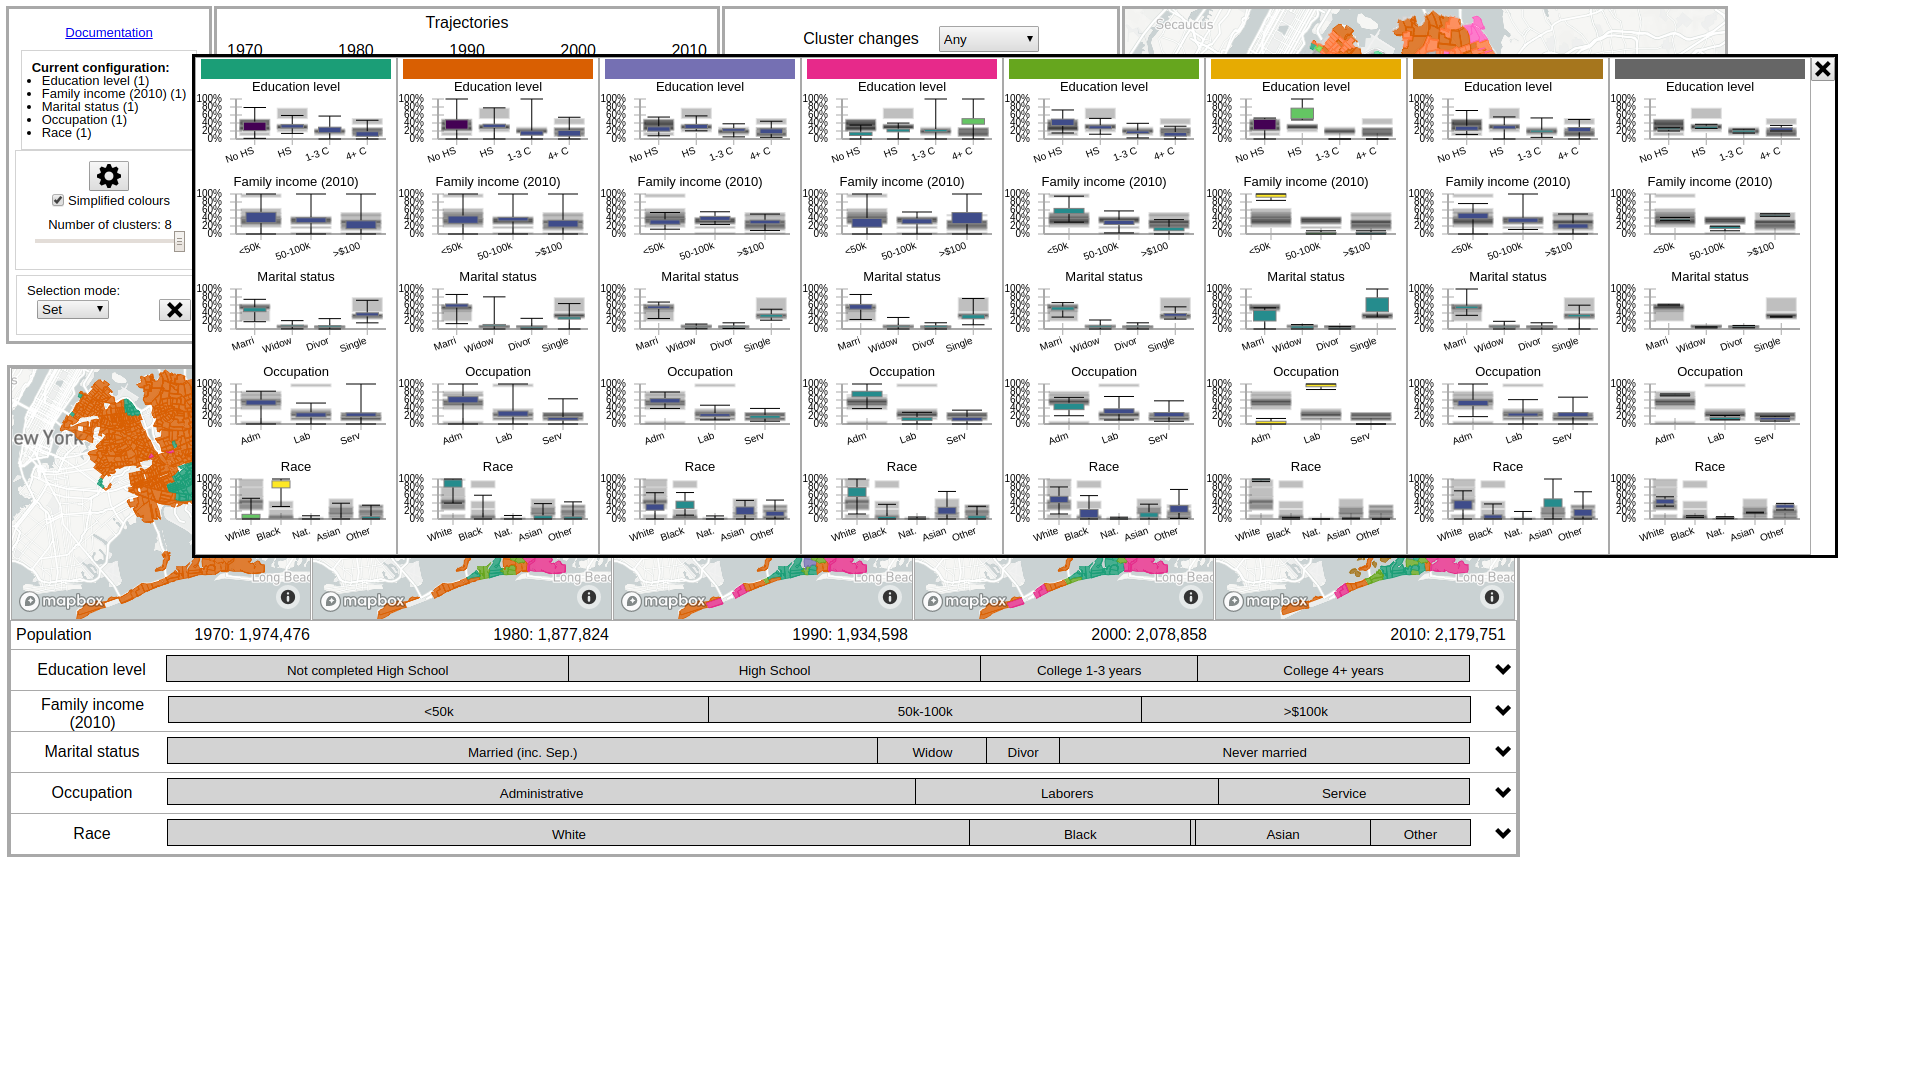
\includegraphics[width=\linewidth]{13b.png}
\end{center} \clearpage



\subsection{The Bronx}
\begin{center}
	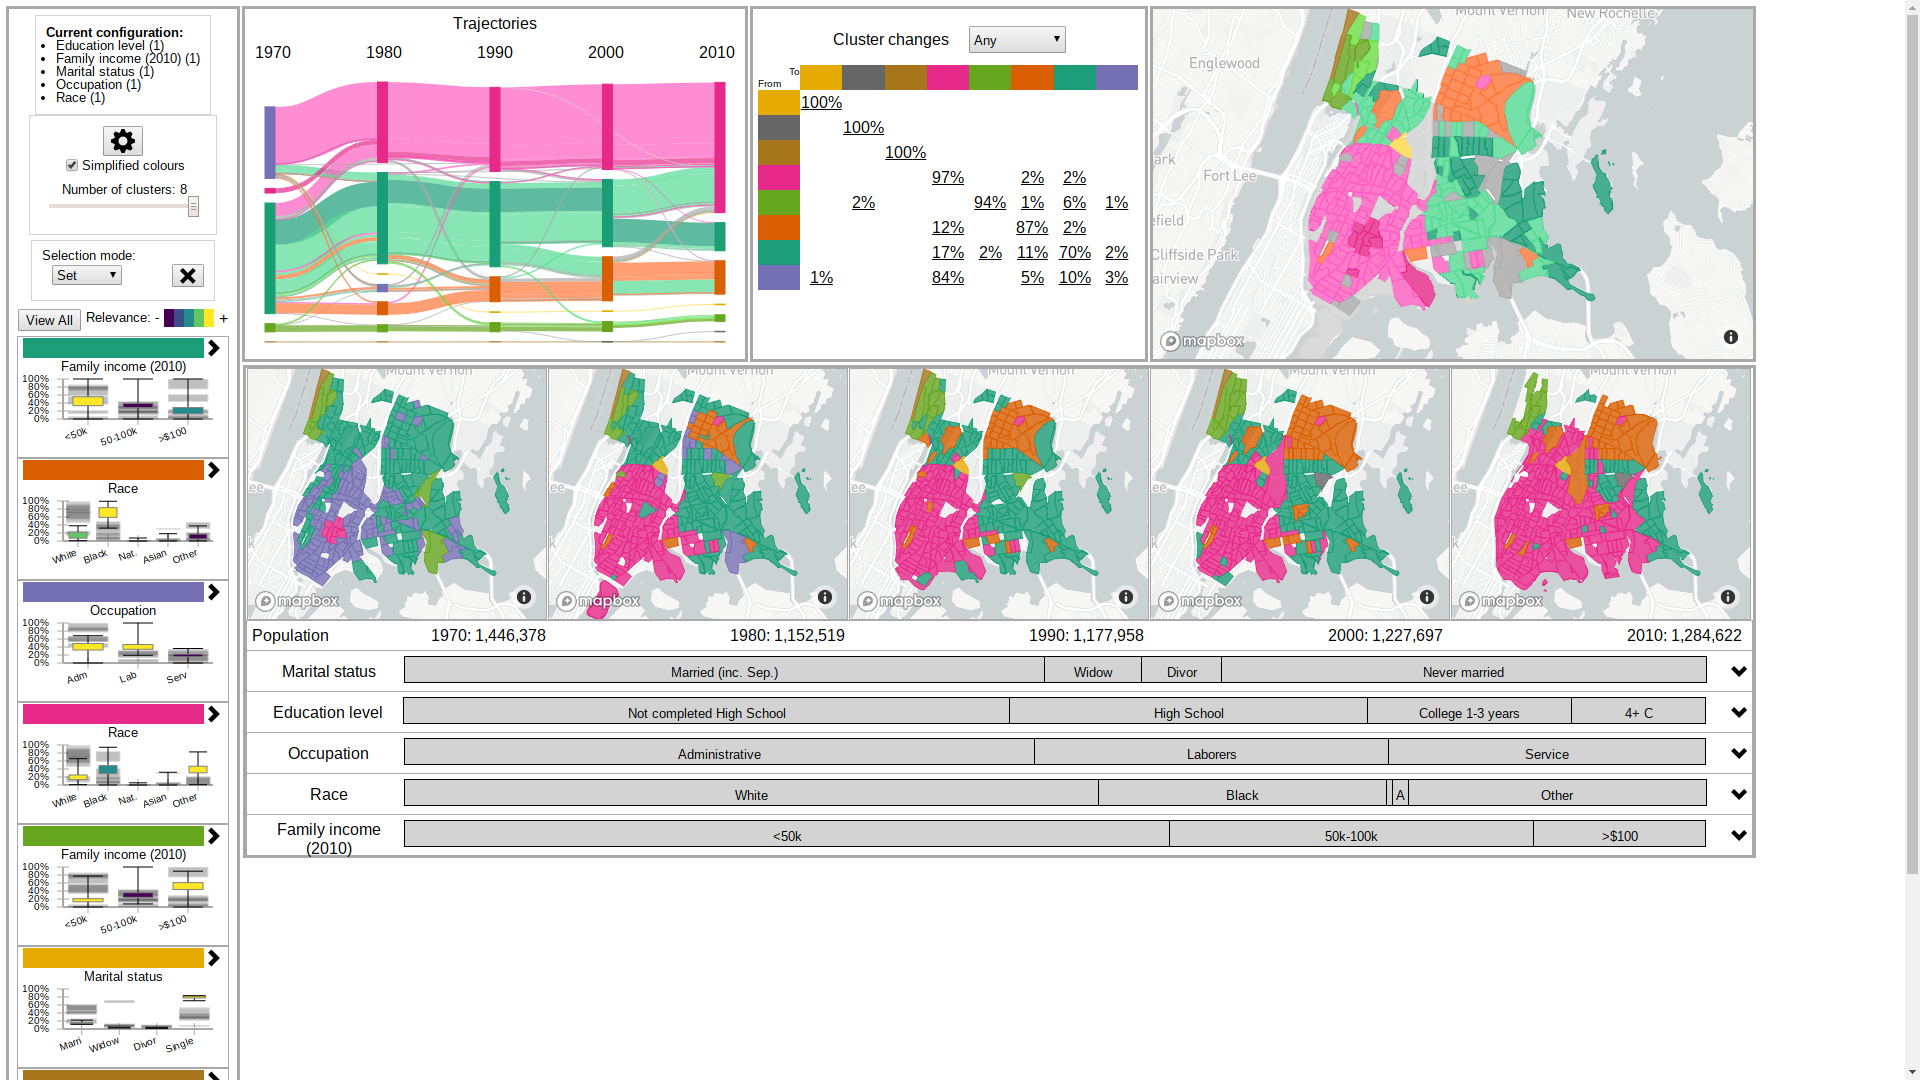
\includegraphics[width=\linewidth]{14a.png}
	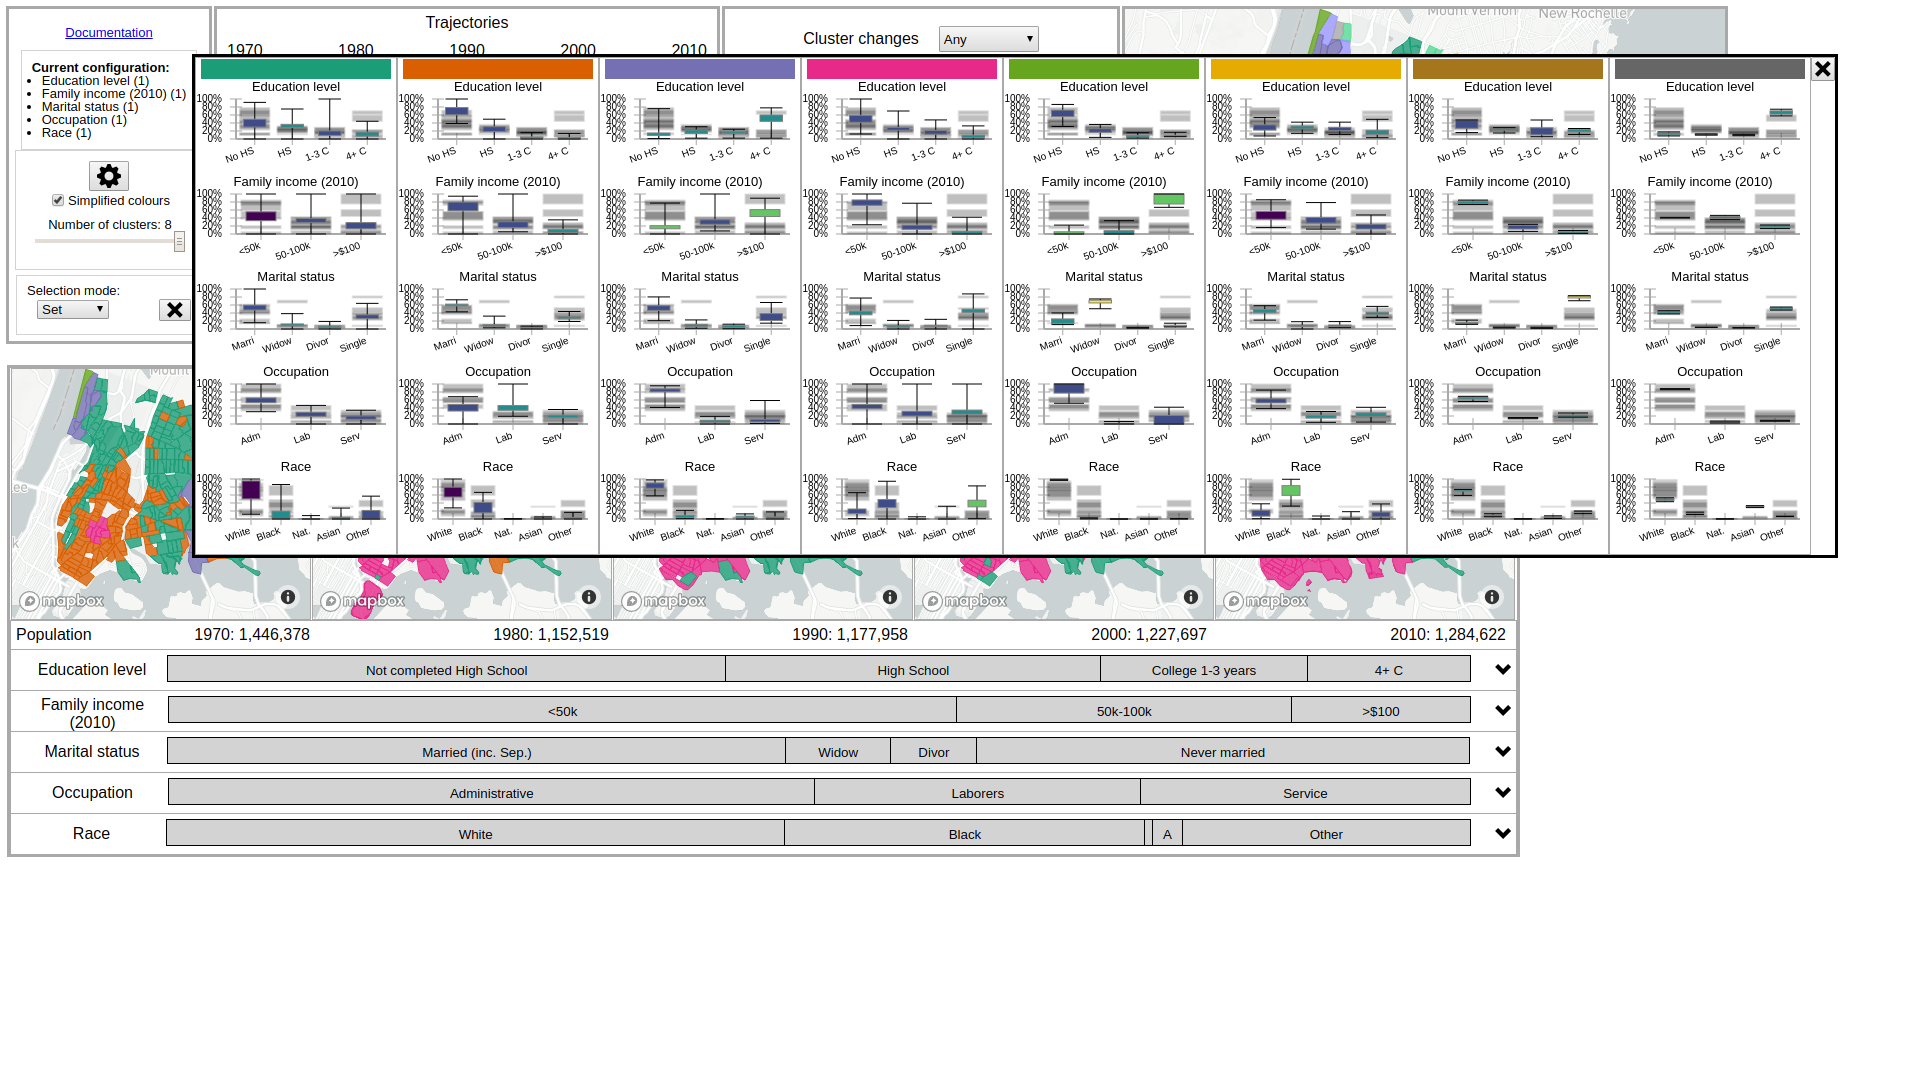
\includegraphics[width=\linewidth]{14b.png}
\end{center} \clearpage



\subsection{Brooklyn}
\begin{center}
	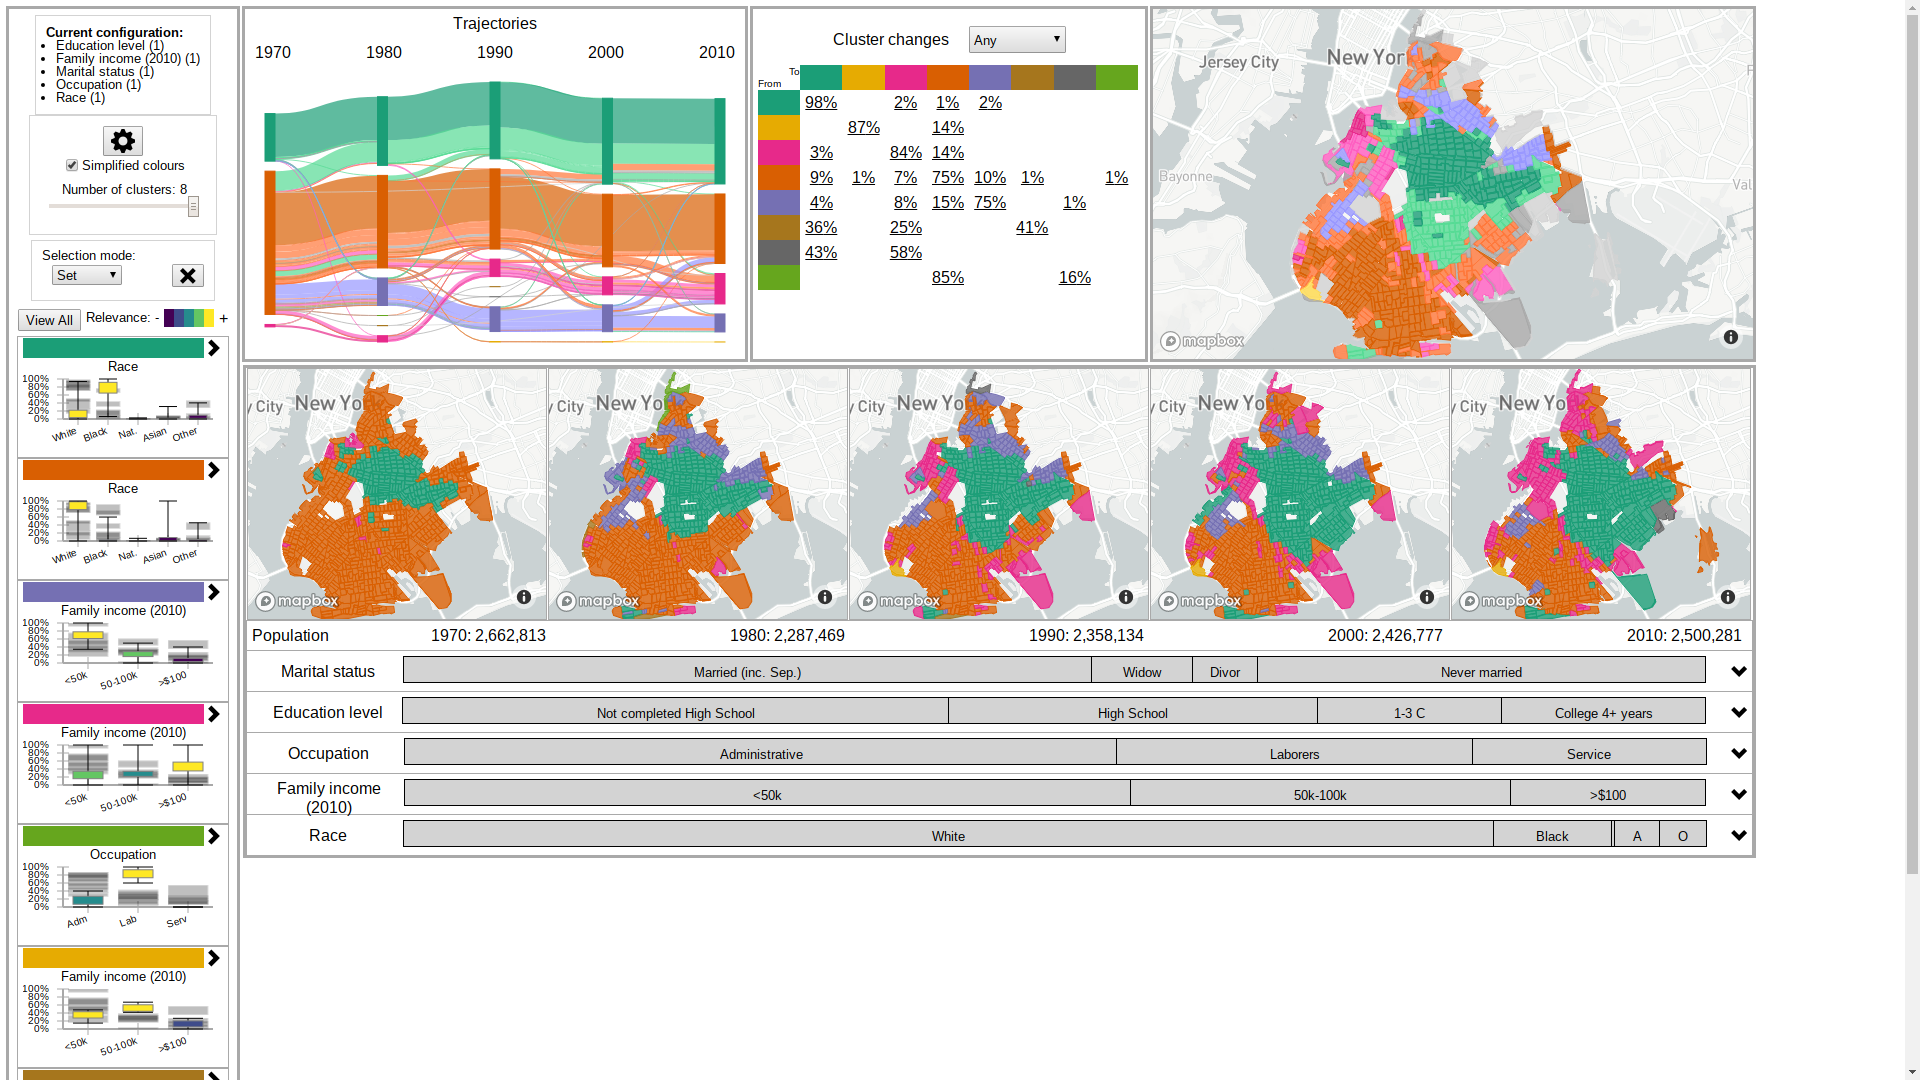
\includegraphics[width=\linewidth]{15a.png}
	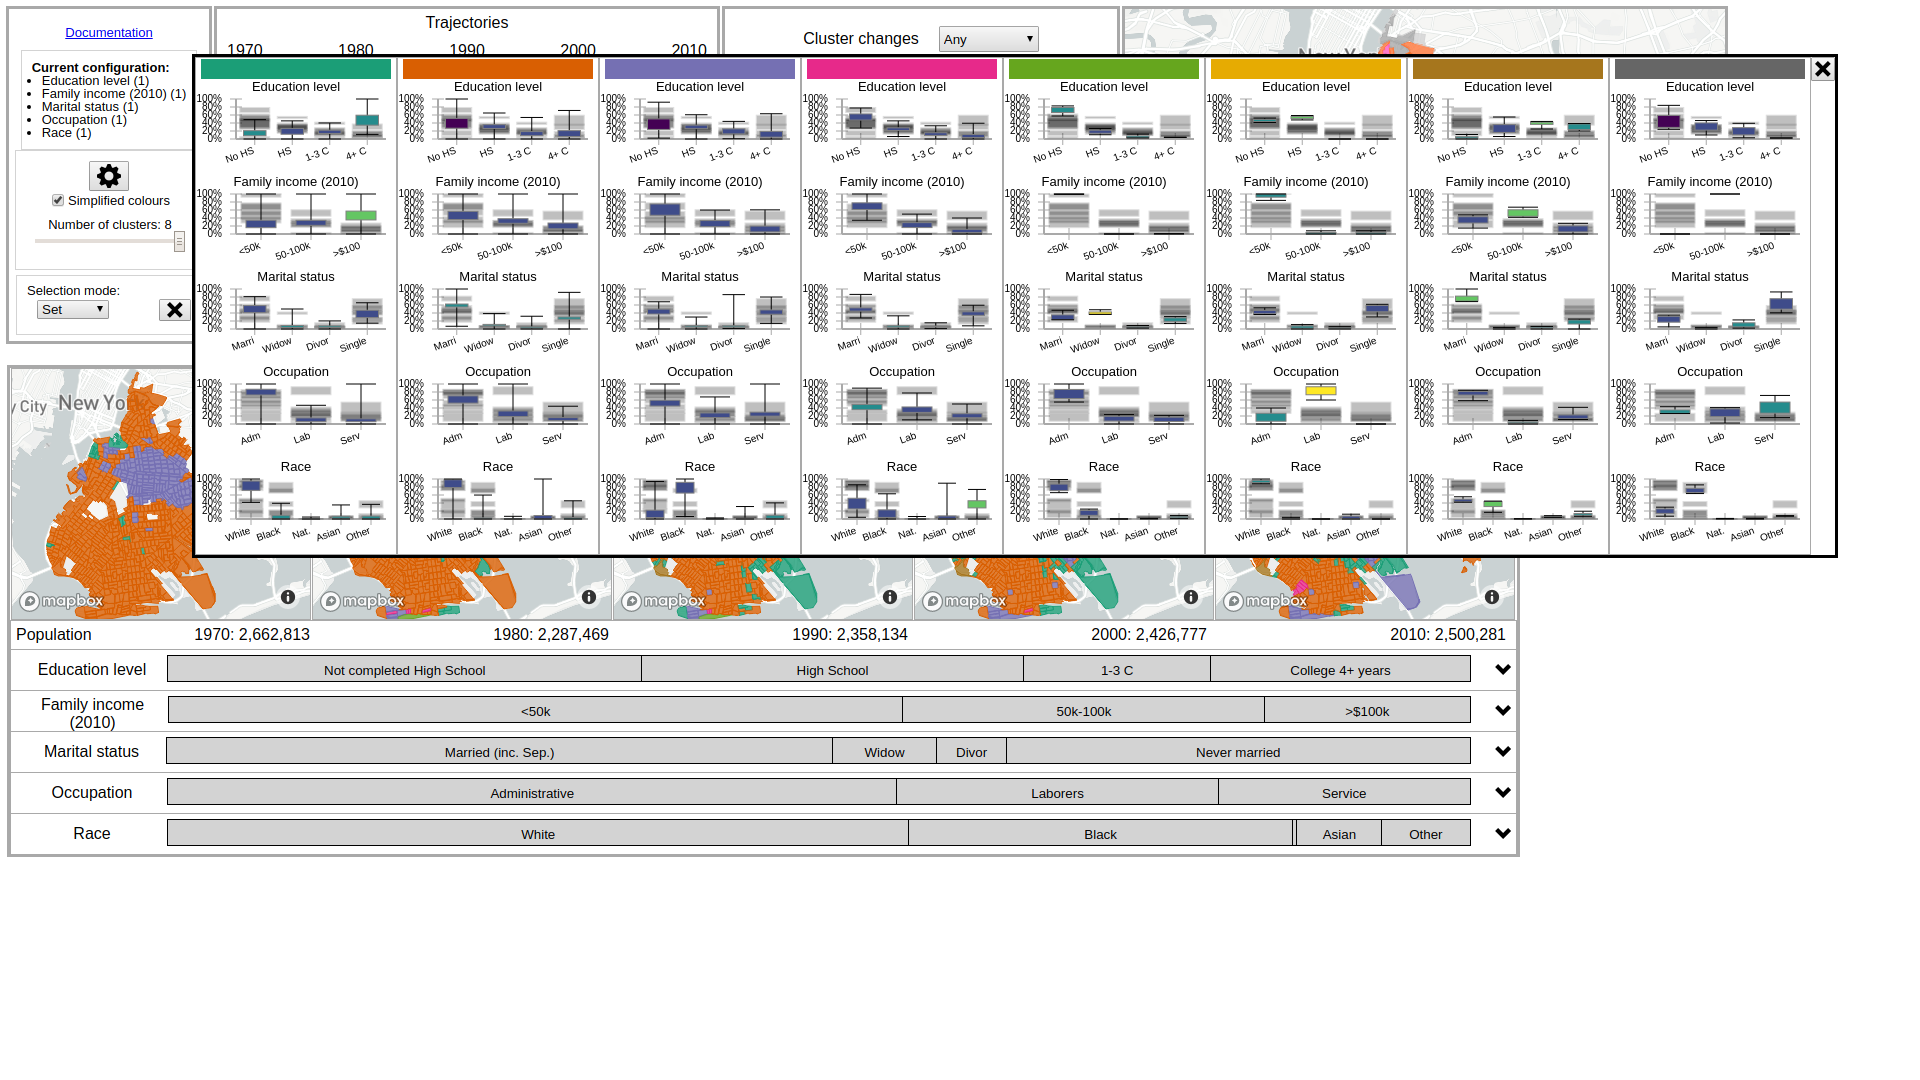
\includegraphics[width=\linewidth]{15b.png}
\end{center} \clearpage



\subsection{Chicago}
\begin{center}
	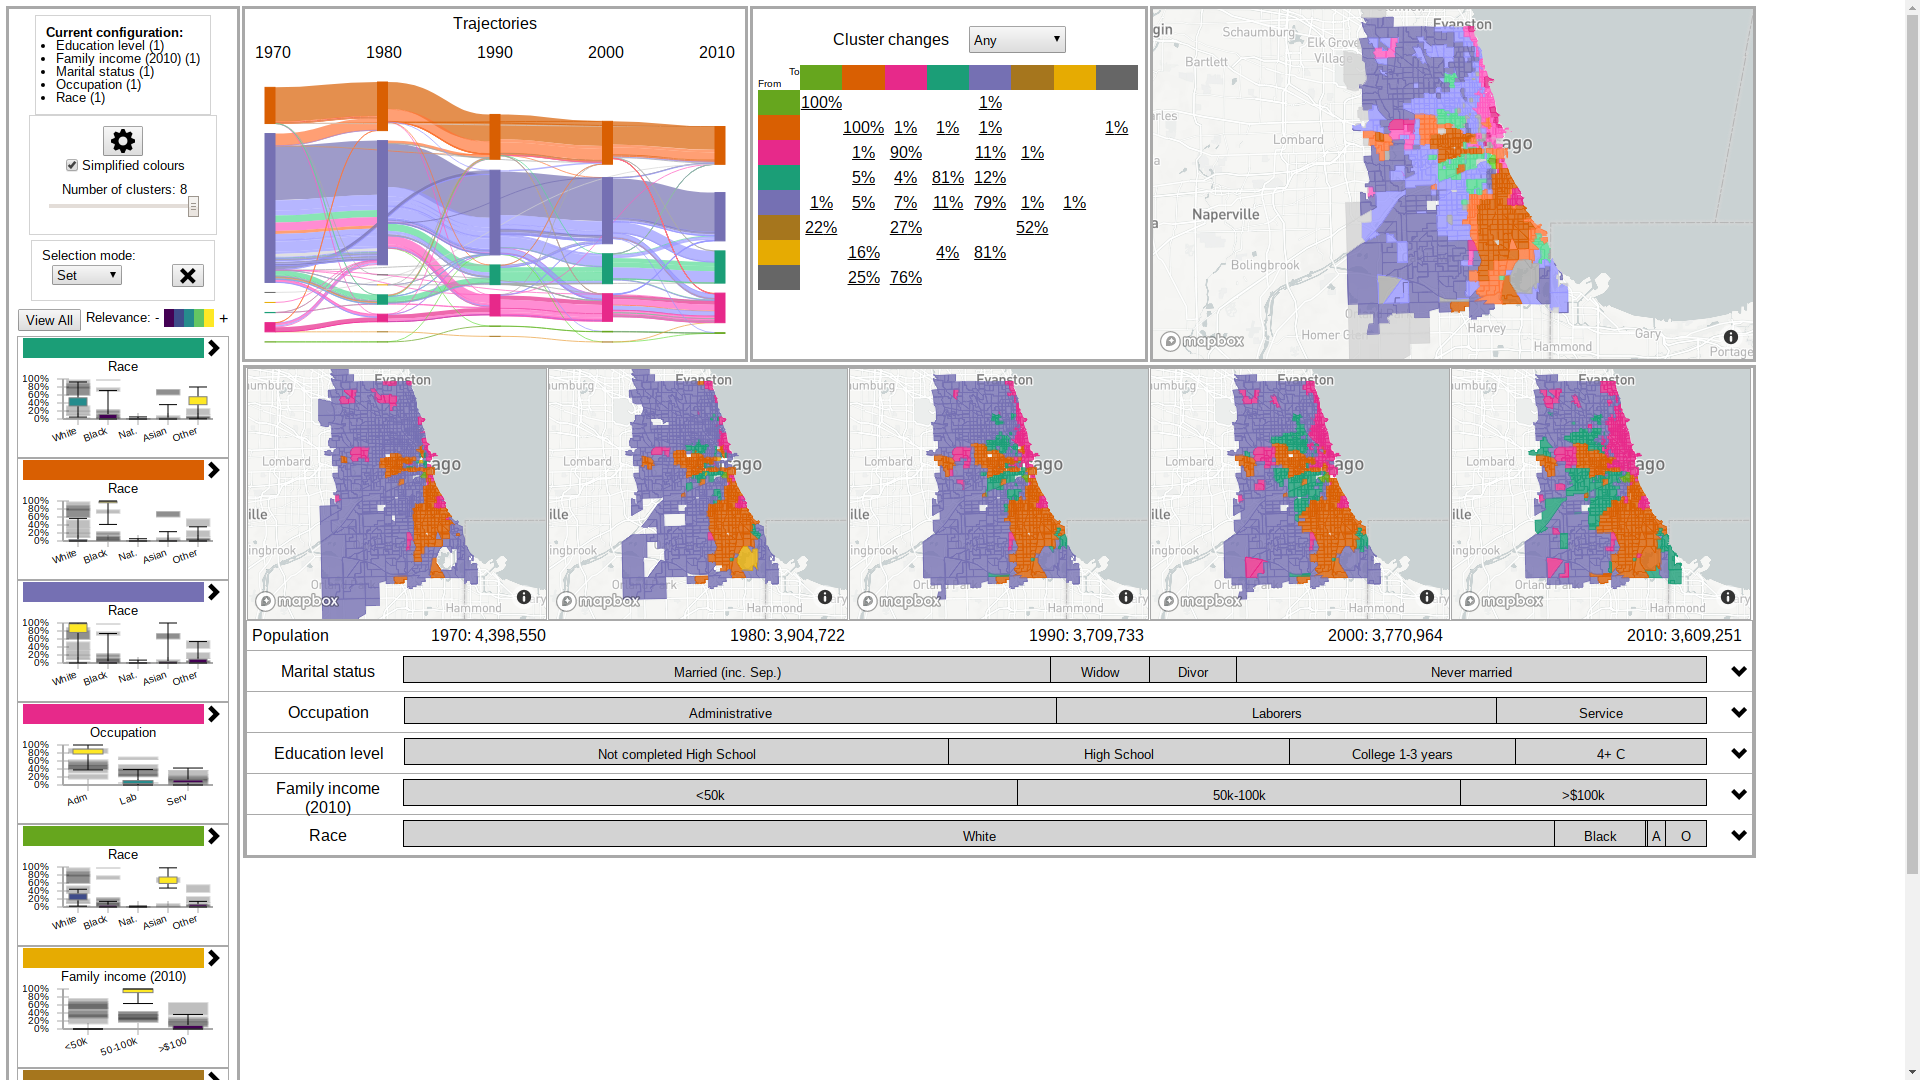
\includegraphics[width=\linewidth]{16a.png}
	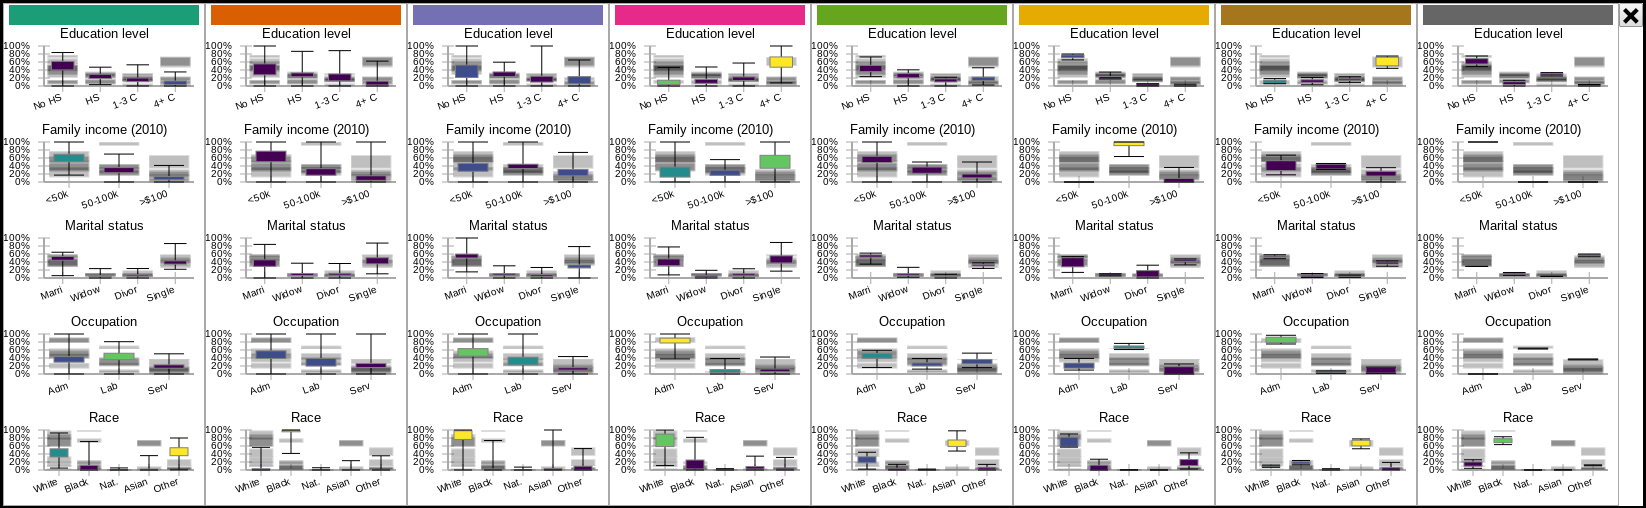
\includegraphics[width=\linewidth]{16b.png}
\end{center} \clearpage



\subsection{Atlanta}
\begin{center}
	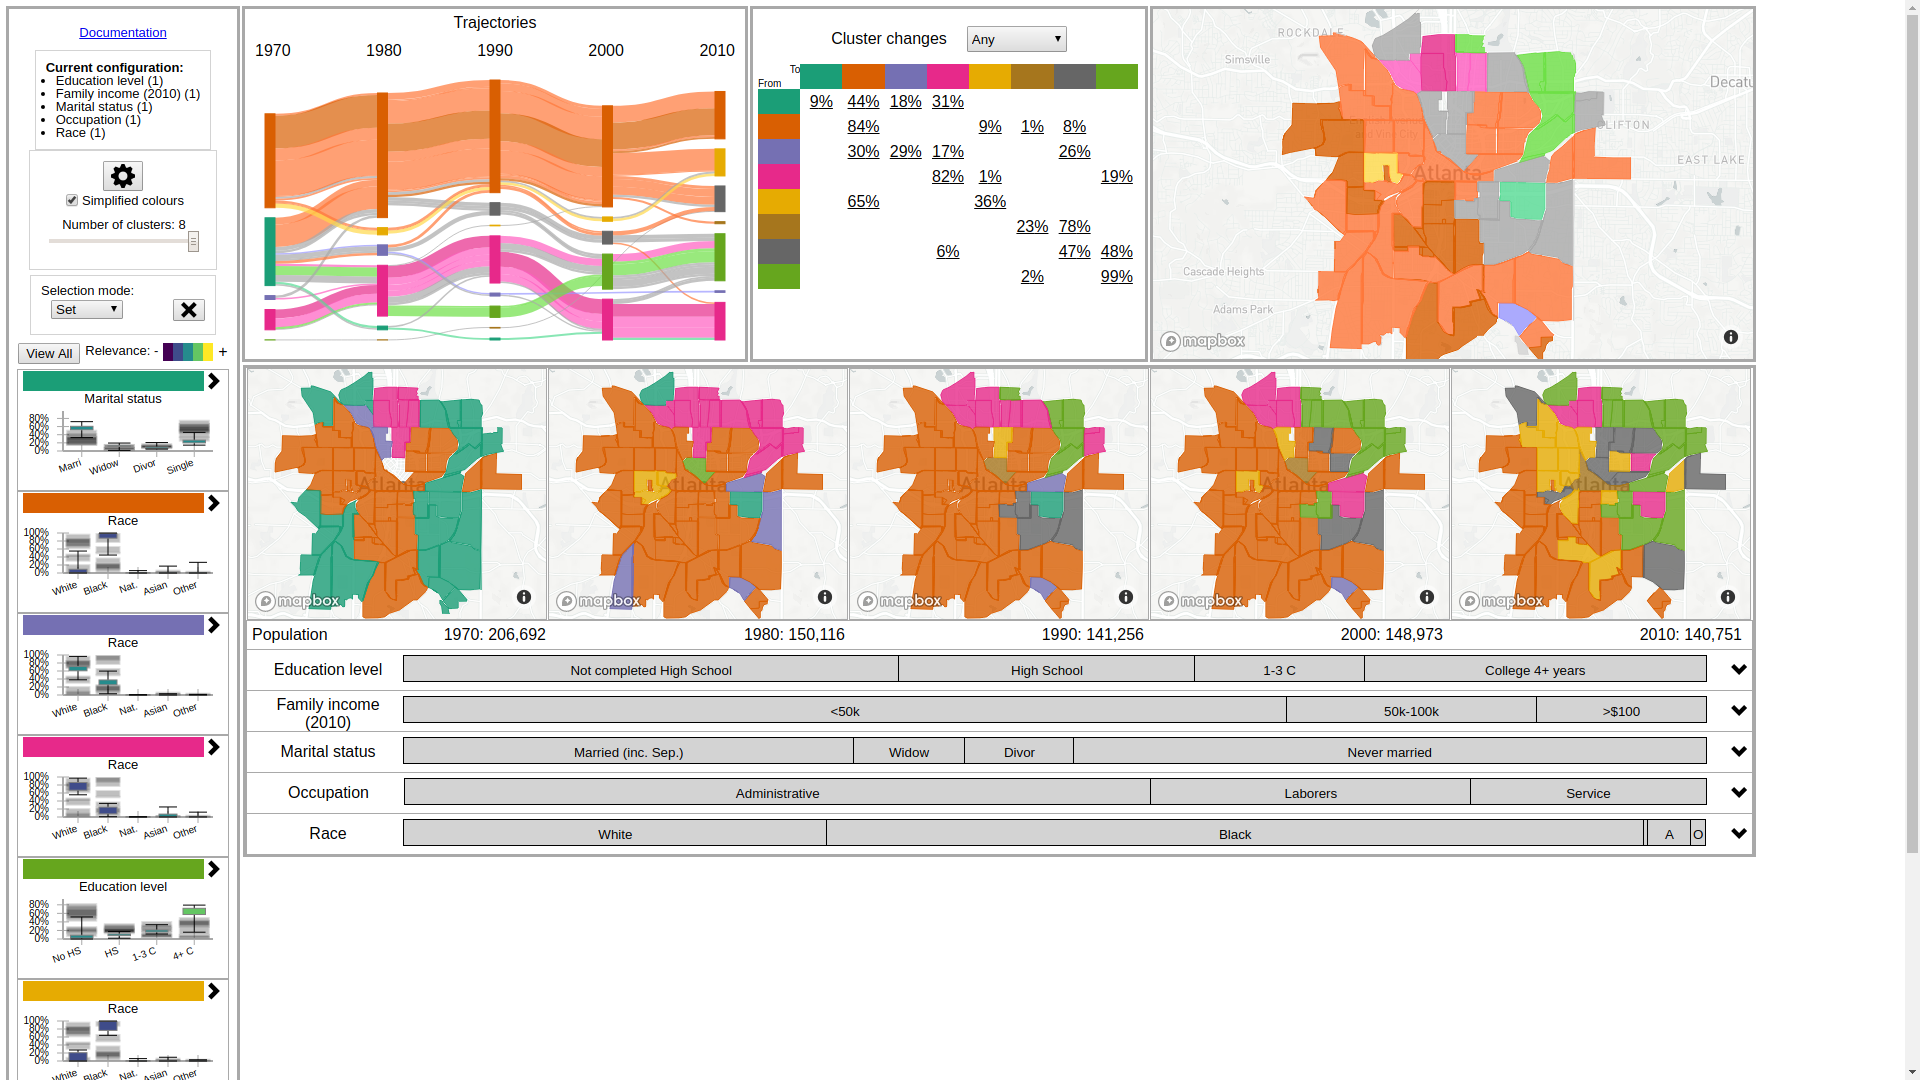
\includegraphics[width=\linewidth]{17a.png}
	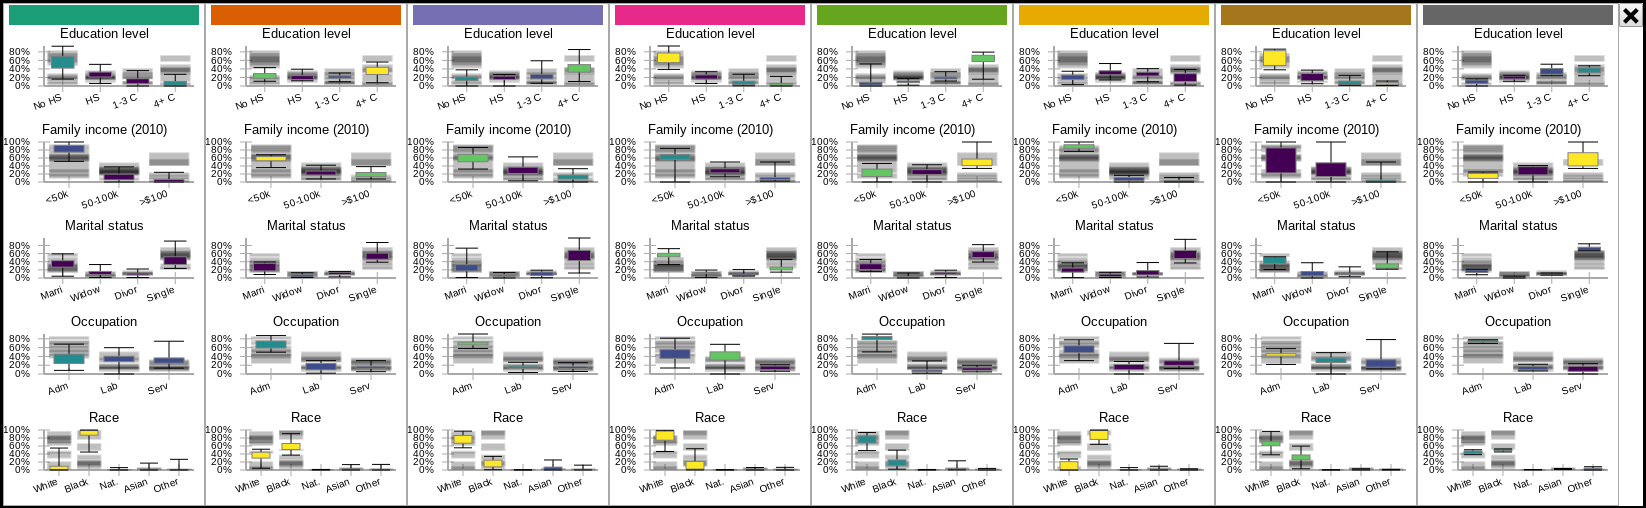
\includegraphics[width=\linewidth]{17b.png}
\end{center} \clearpage



\subsection{Austin}
\begin{center}
	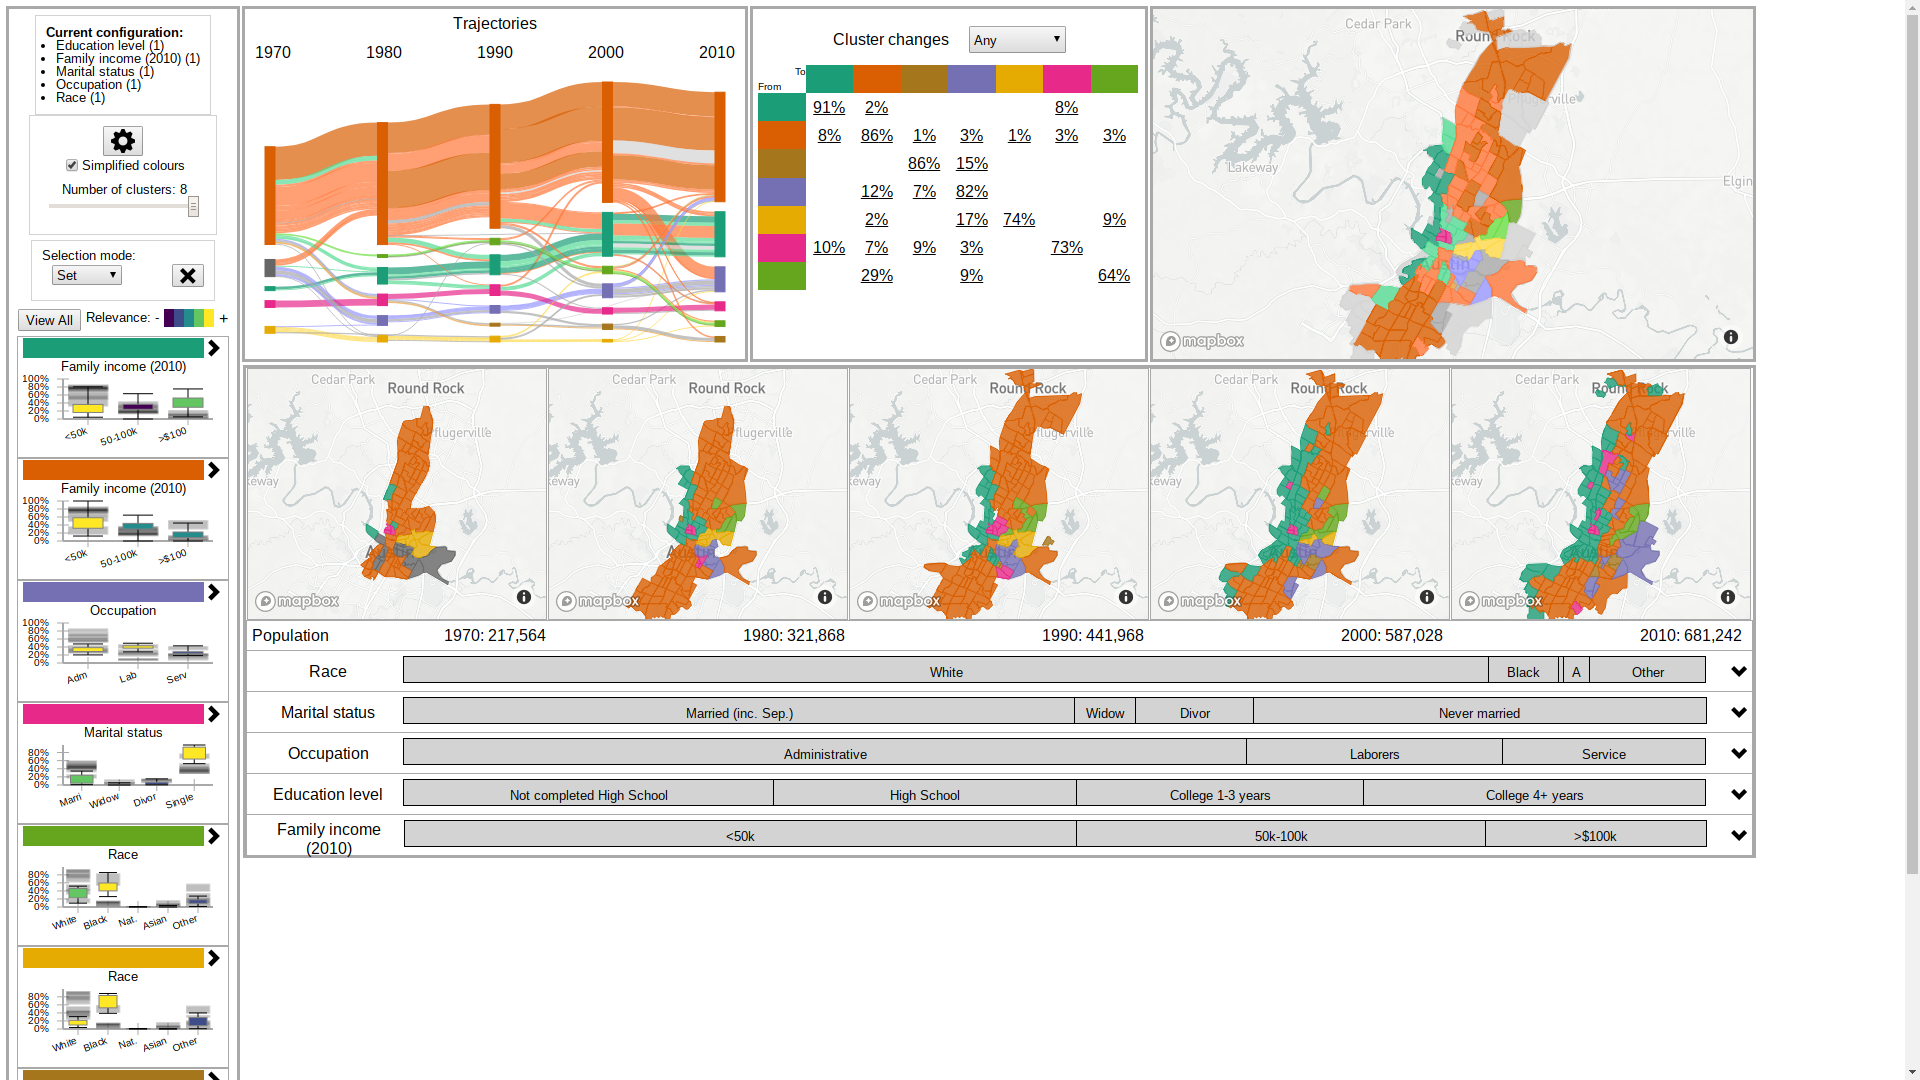
\includegraphics[width=\linewidth]{18a.png}
	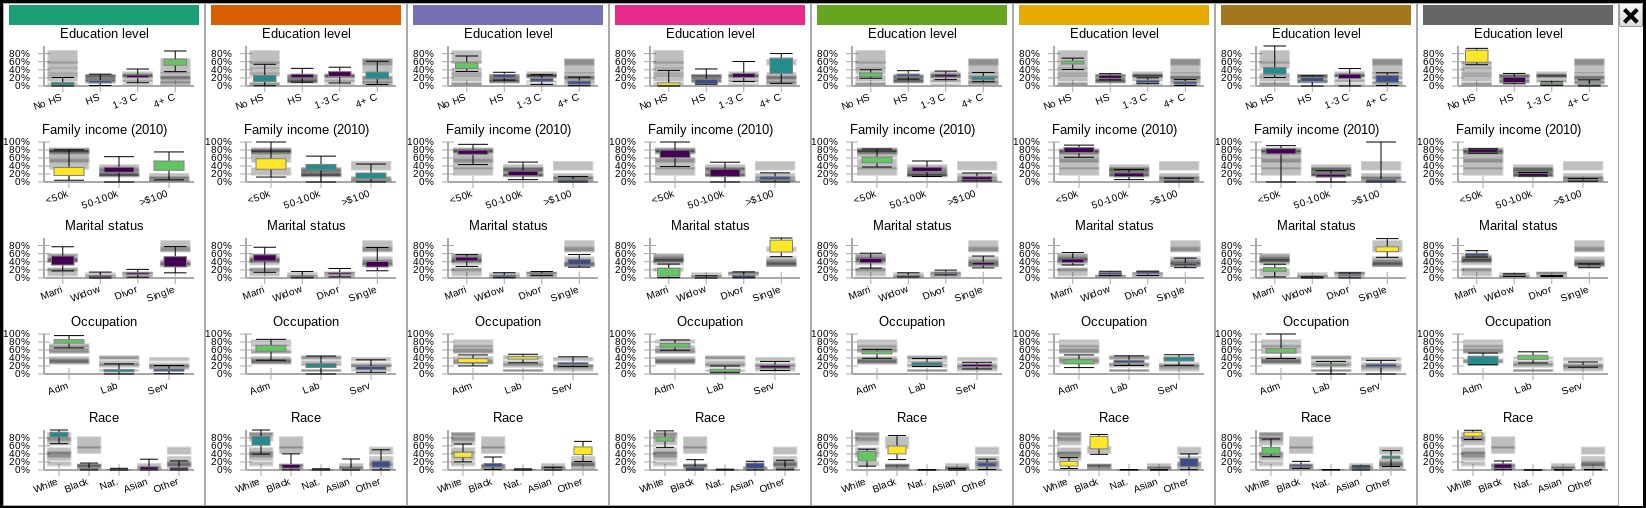
\includegraphics[width=\linewidth]{18b.png}
\end{center} \clearpage



\subsection{Baltimore}
\begin{center}
	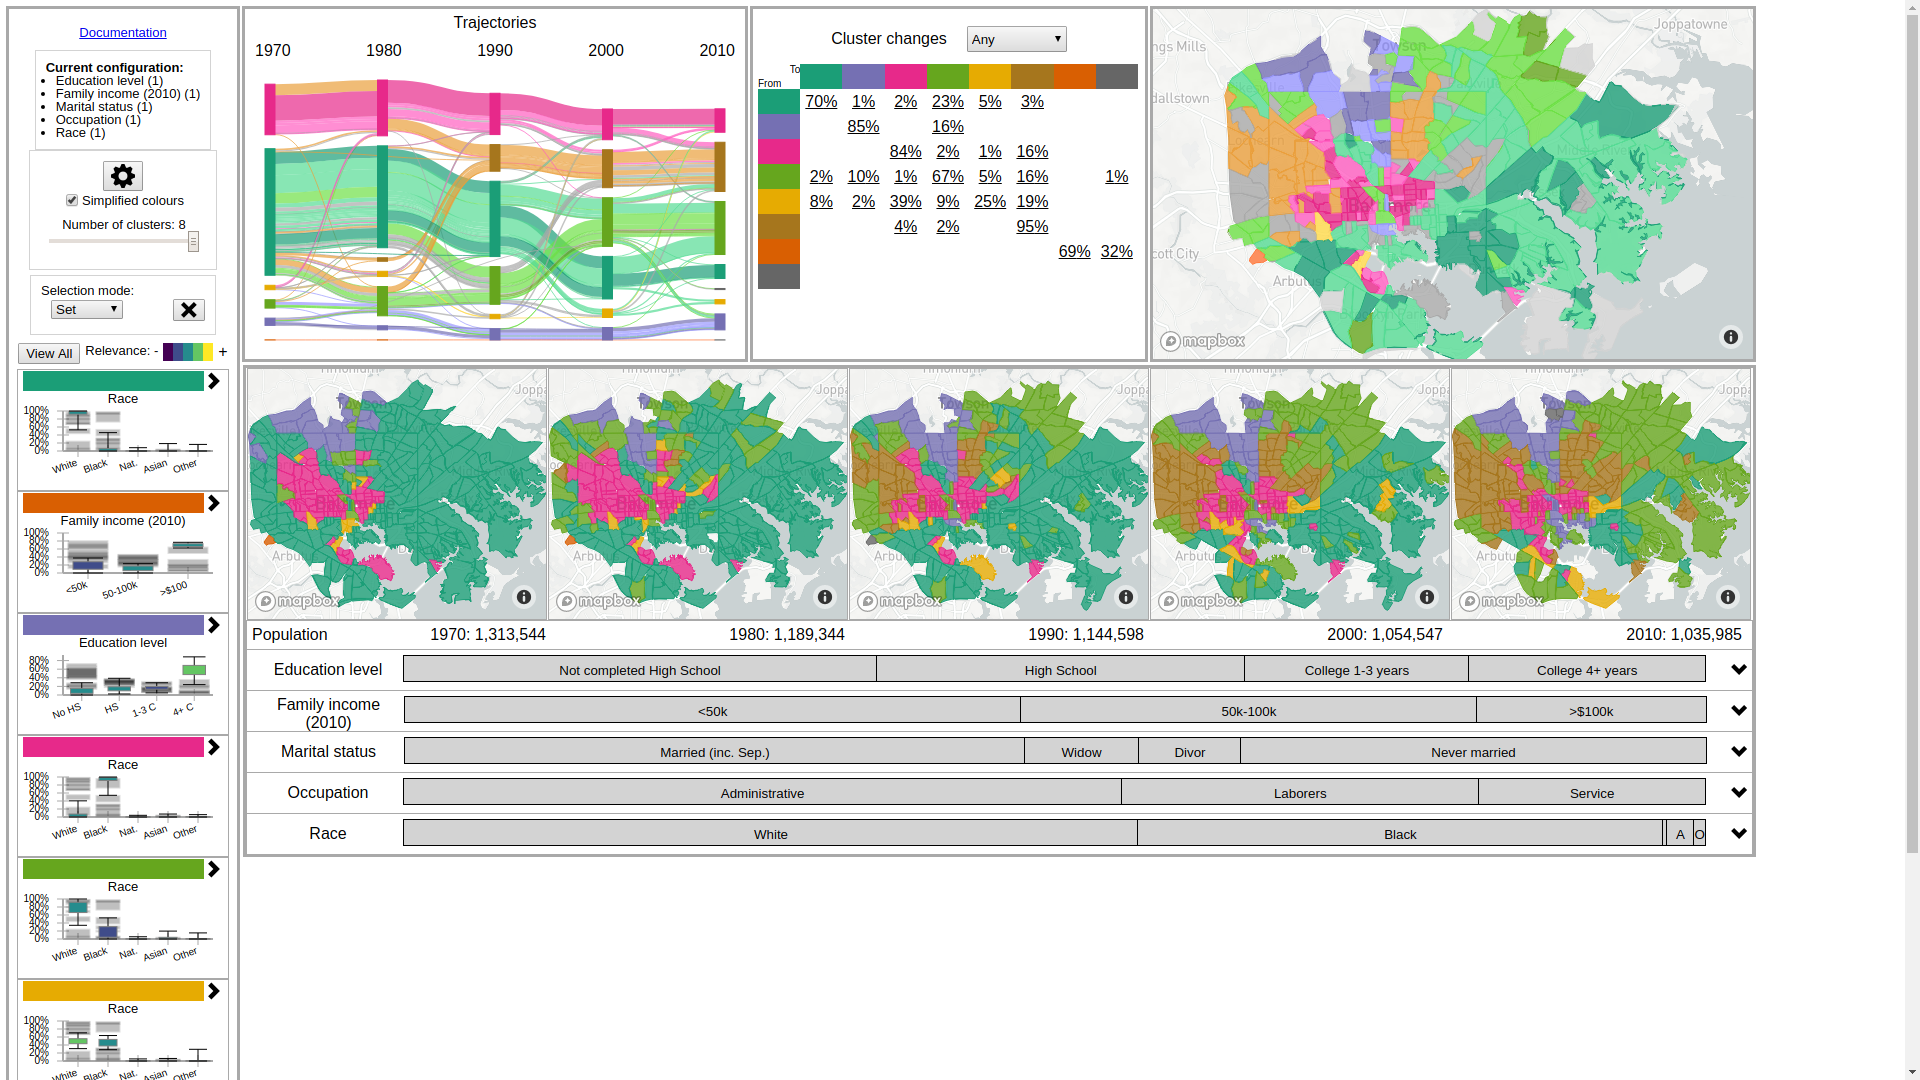
\includegraphics[width=\linewidth]{19a.png}
	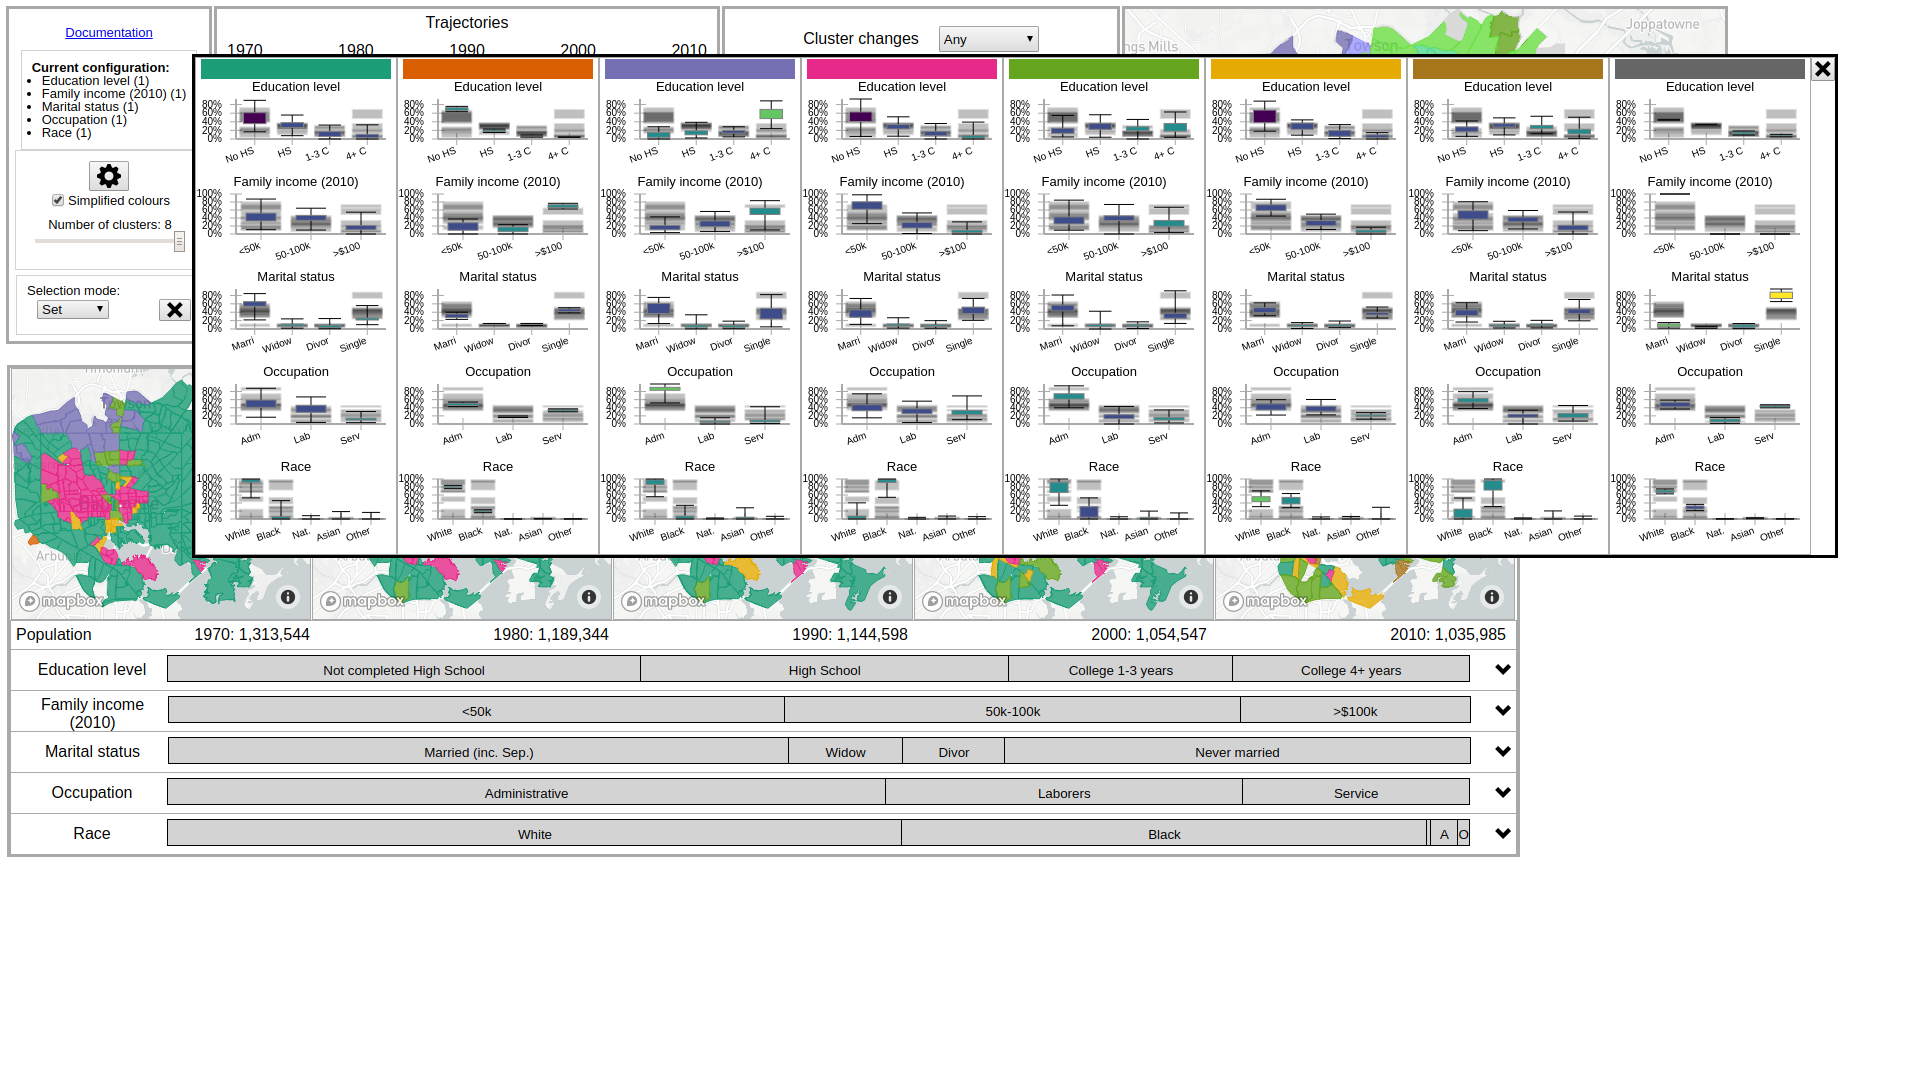
\includegraphics[width=\linewidth]{19b.png}
\end{center} \clearpage



\subsection{Boston}
\begin{center}
	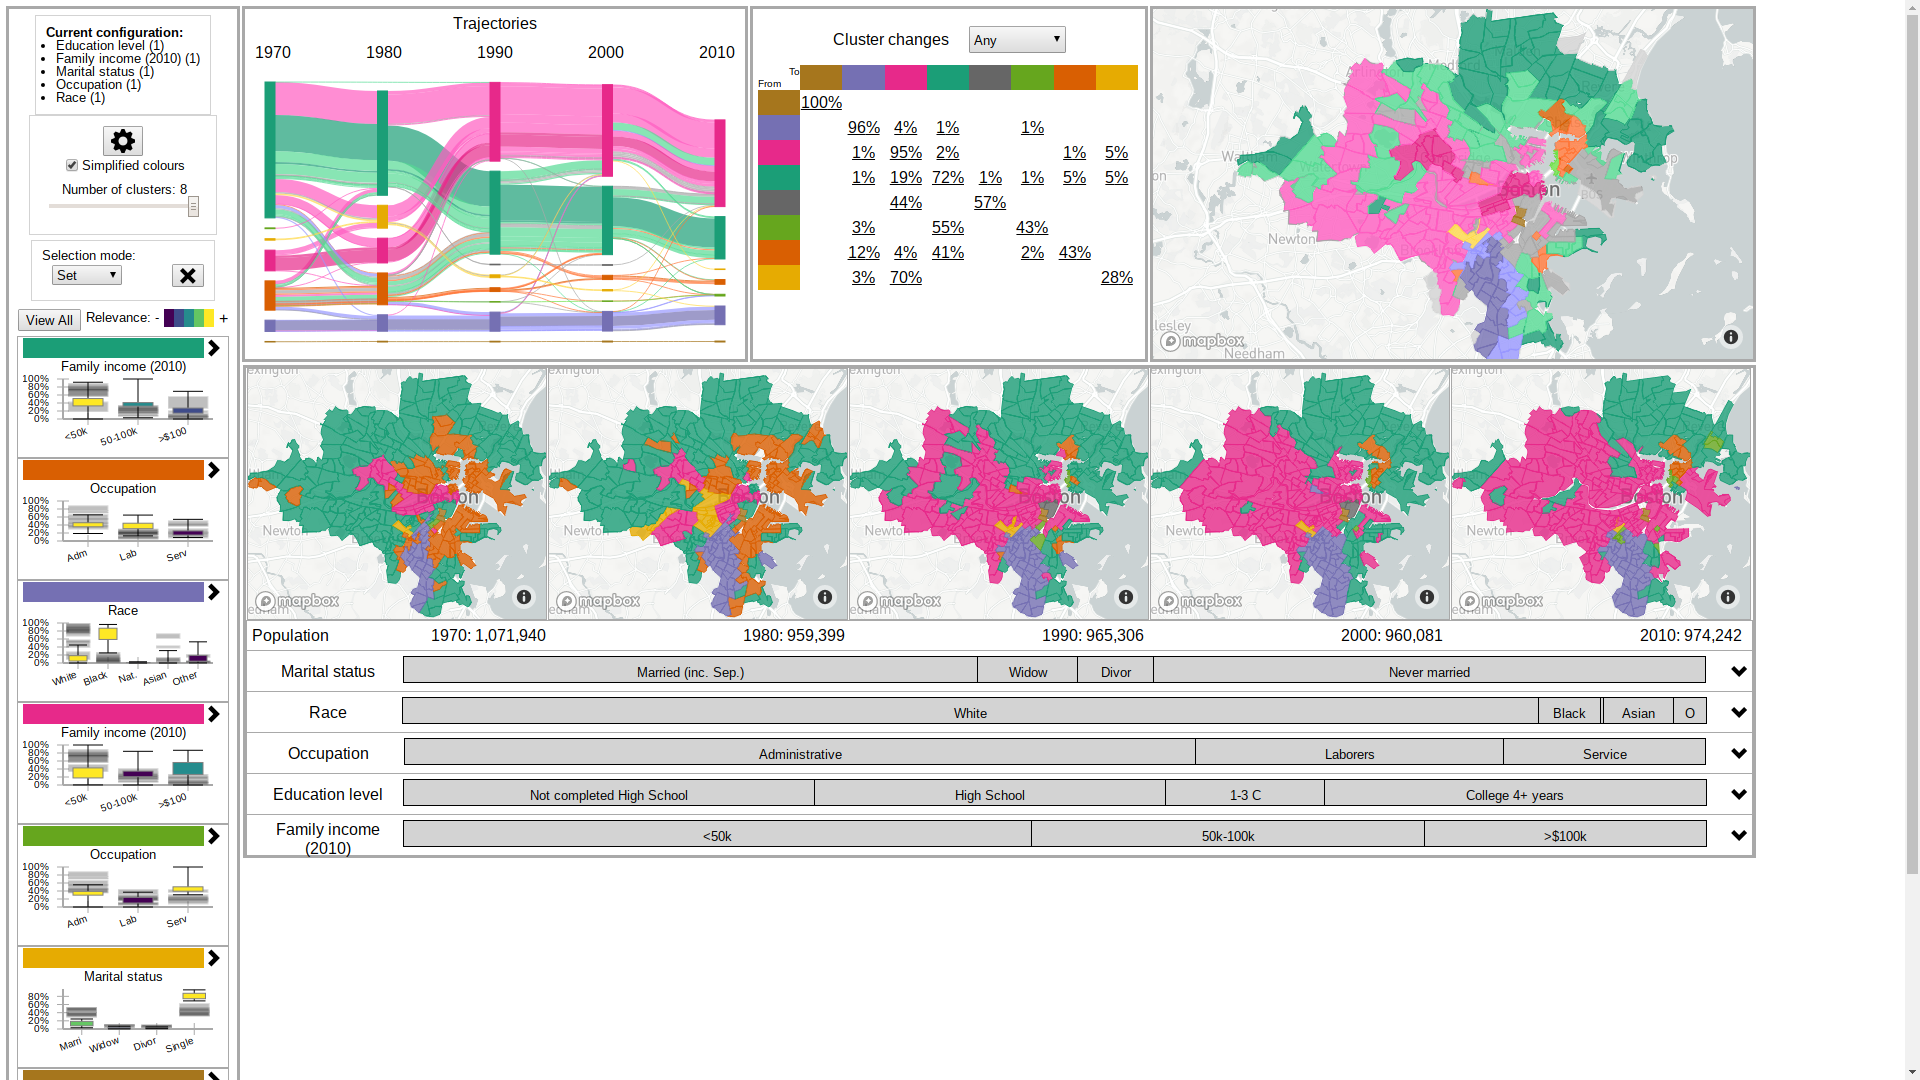
\includegraphics[width=\linewidth]{20a.png}
	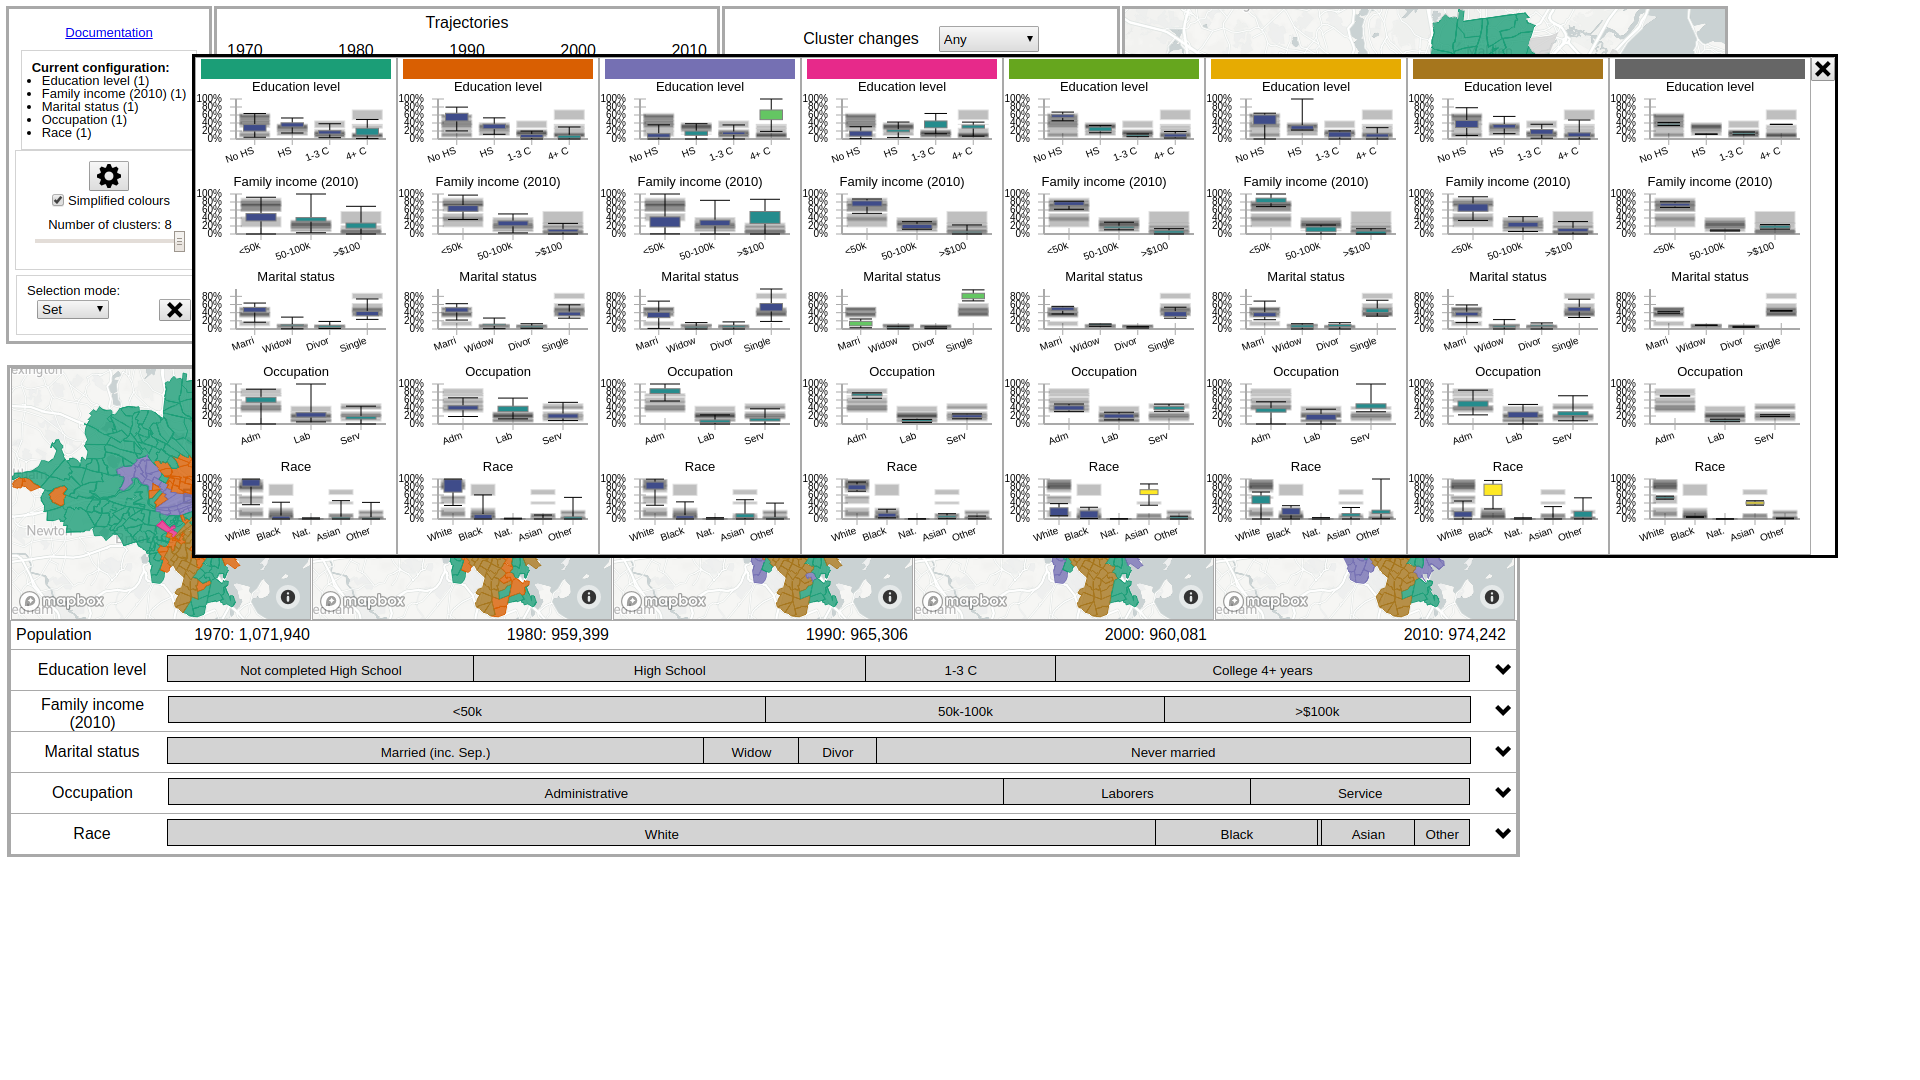
\includegraphics[width=\linewidth]{20b.png}
\end{center} \clearpage



\subsection{Columbus}
\begin{center}
	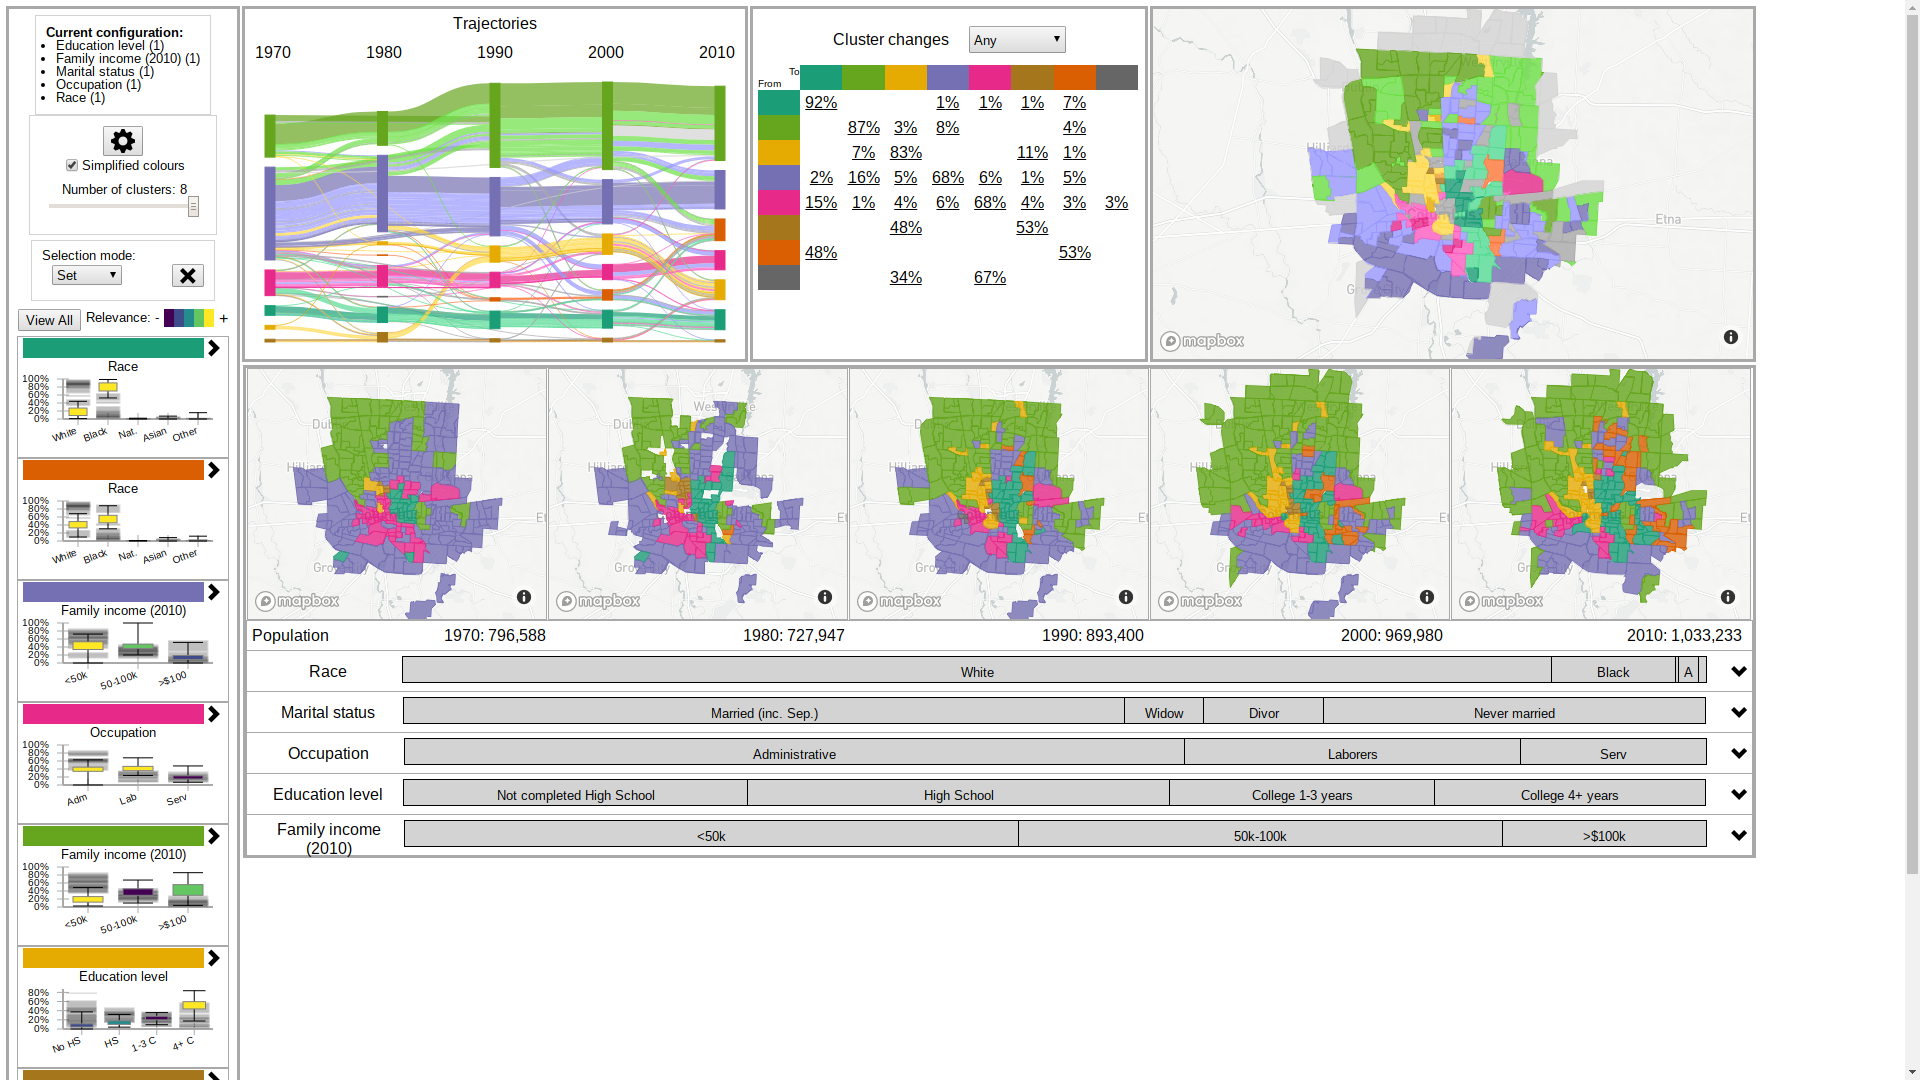
\includegraphics[width=\linewidth]{21a.png}
	\includegraphics[width=\linewidth]{21b.png}
\end{center} \clearpage



\subsection{Dallas}
\begin{center}
	\includegraphics[width=\linewidth]{22a.png}
	\includegraphics[width=\linewidth]{22b.png}
\end{center} \clearpage



\subsection{Denver}
\begin{center}
	\includegraphics[width=\linewidth]{23a.png}
	\includegraphics[width=\linewidth]{23b.png}
\end{center} \clearpage



\subsection{Fargo}
\begin{center}
	\includegraphics[width=\linewidth]{24a.png}
	\includegraphics[width=\linewidth]{24b.png}
\end{center} \clearpage



\subsection{Houston}
\begin{center}
	\includegraphics[width=\linewidth]{25a.png}
	\includegraphics[width=\linewidth]{25b.png}
\end{center} \clearpage



\subsection{Indianapolis}
\begin{center}
	\includegraphics[width=\linewidth]{26a.png}
	\includegraphics[width=\linewidth]{26b.png}
\end{center} \clearpage



\subsection{Jacksonville}
\begin{center}
	\includegraphics[width=\linewidth]{27a.png}
	\includegraphics[width=\linewidth]{27b.png}
\end{center} \clearpage



\subsection{Kansas City}
\begin{center}
	\includegraphics[width=\linewidth]{28a.png}
	\includegraphics[width=\linewidth]{28b.png}
\end{center} \clearpage



\subsection{Las Vegas}
\begin{center}
	\includegraphics[width=\linewidth]{29a.png}
	\includegraphics[width=\linewidth]{29b.png}
\end{center} \clearpage



\subsection{Miami}
\begin{center}
	\includegraphics[width=\linewidth]{30a.png}
	\includegraphics[width=\linewidth]{30b.png}
\end{center} \clearpage



\subsection{Minneapolis}
\begin{center}
	\includegraphics[width=\linewidth]{31a.png}
	\includegraphics[width=\linewidth]{31b.png}
\end{center} \clearpage



\subsection{Philadelphia}
\begin{center}
	\includegraphics[width=\linewidth]{32a.png}
	\includegraphics[width=\linewidth]{32b.png}
\end{center} \clearpage



\subsection{Phoenix}
\begin{center}
	\includegraphics[width=\linewidth]{33a.png}
	\includegraphics[width=\linewidth]{33b.png}
\end{center} \clearpage



\subsection{Salt Lake City}
\begin{center}
	\includegraphics[width=\linewidth]{34a.png}
	\includegraphics[width=\linewidth]{34b.png}
\end{center} \clearpage



\subsection{San Antonio}
\begin{center}
	\includegraphics[width=\linewidth]{35a.png}
	\includegraphics[width=\linewidth]{35b.png}
\end{center} \clearpage



\subsection{San Francisco}
\begin{center}
	\includegraphics[width=\linewidth]{36a.png}
	\includegraphics[width=\linewidth]{36b.png}
\end{center} \clearpage



\subsection{Seattle}
\begin{center}
	\includegraphics[width=\linewidth]{37a.png}
	\includegraphics[width=\linewidth]{37b.png}
\end{center} \clearpage



\subsection{Washington DC}
\begin{center}
	\includegraphics[width=\linewidth]{38a.png}
	\includegraphics[width=\linewidth]{38b.png}
\end{center} 


\end{document}
